% Capitolul 5b: Modele GARCH Multivariate
% Prezentare academică de calitate Harvard
% Program de licență, Academia de Studii Economice din București

\documentclass[9pt, aspectratio=169, t]{beamer}
\input{preamble}
\subtitle{Capitolul 5b: Modele GARCH Multivariate}

\begin{document}

% Pagina de titlu (fără antet/subsol)
{
\setbeamertemplate{headline}{}
\setbeamertemplate{footline}{}
\begin{frame}
    \titlepage
\end{frame}
}

%=============================================================================
% OBIECTIVE DE ÎNVĂȚARE
%=============================================================================
\section{Motivație}

\begin{frame}{Obiective de învățare}
    \begin{cminipage}{0.95\textwidth}
    {\footnotesize
    \begin{block}{La finalul acestui capitol, veți fi capabili să:}
        \begin{enumerate}\setlength{\itemsep}{2pt}
            \item Explicați de ce \textbf{modelarea multivariată a volatilității} este necesară
            \item Formulați și estimați modele \textbf{VEC}, \textbf{BEKK}, \textbf{CCC} și \textbf{DCC}
            \item Interpretați \textbf{corelații dinamice} și descompuneri ale covarianței
            \item Aplicați GARCH multivariat pentru \textbf{optimizare de portofoliu}, \textbf{hedging} și \textbf{managementul riscului}
        \end{enumerate}
    \end{block}
    \vspace{0.1cm}
    \begin{alertblock}{Competențe practice}
        \begin{itemize}\setlength{\itemsep}{0pt}
            \item Implementare Python cu pachetele \texttt{rmgarch} / \texttt{mgarch}
            \item Interpretarea matricelor de covarianță variabile în timp
            \item Rapoarte de hedging dinamic și ponderi de portofoliu
        \end{itemize}
    \end{alertblock}
    \vspace{0.2cm}
    \textit{\textbf{Concluzie cheie:} Nu învățați modele --- învățați cum să măsurați riscul real de portofoliu.}
    }
    \end{cminipage}
\end{frame}

%=============================================================================
% CUPRINS
%=============================================================================
\begin{frame}{Cuprins}
    \vspace{-0.3cm}
    {\small
    \begin{columns}[T]
        \begin{column}{0.48\textwidth}
            \begin{block}{Fundamente}
                \begin{itemize}\setlength{\itemsep}{3pt}
                    \item Motivație: De la univariat la multivariat
                    \item Cadrul GARCH multivariat
                    \item Modele VEC și VEC diagonal
                    \item Modelul BEKK
                    \item Corelația condițională constantă (CCC)
                    \item Corelația condițională dinamică (DCC)
                \end{itemize}
            \end{block}
        \end{column}
        \begin{column}{0.48\textwidth}
            \begin{exampleblock}{Aplicații}
                \begin{itemize}\setlength{\itemsep}{3pt}
                    \item Alte modele GARCH multivariate
                    \item Estimare și \textit{curse of dimensionality}
                    \item Studii de caz pe date reale
                    \item Optimizare de portofoliu
                    \item Hedging dinamic și VaR
                    \item Rezumat și Test
                \end{itemize}
            \end{exampleblock}
        \end{column}
    \end{columns}
    }
\end{frame}

%=============================================================================
% POVESTEA CAPITOLULUI
%=============================================================================

\begin{frame}{Povestea acestui capitol: problema}
    \begin{cminipage}{0.95\textwidth}
    {\footnotesize
    \textit{\textbf{Întrebare fundamentală:} Cum modelăm riscul când activele se mișcă împreună --- și acea co-mișcare se schimbă în timp?}
    \vspace{0.2cm}
    \begin{block}{Problema}
        \begin{itemize}\setlength{\itemsep}{2pt}
            \item Corelațiile dintre active \textbf{se schimbă în timp} --- și cresc brusc în perioade de criză
            \item Ignorarea lor duce la portofolii greșite, hedging ineficient și risc subestimat
        \end{itemize}
    \end{block}
    \vspace{0.1cm}
    \begin{alertblock}{Dificultatea}
        \begin{itemize}\setlength{\itemsep}{2pt}
            \item Modelarea a $N$ active necesită $N(N+1)/2$ elemente de covarianță variabile în timp
            \item \textbf{Blestemul dimensionalității} face cele mai multe abordări infezabile
            \item Matricea de covarianță trebuie să fie \textbf{pozitiv definită} la fiecare pas
        \end{itemize}
    \end{alertblock}
    }
    \end{cminipage}
\end{frame}

\begin{frame}{Povestea acestui capitol: soluțiile}
    \begin{cminipage}{0.95\textwidth}
    {\footnotesize
    \textit{\textbf{Foaie de parcurs:} Fiecare model rezolvă o problemă dar creează alta --- până la DCC.}
    \vspace{0.2cm}
    \begin{block}{De la general la practic}
        \begin{itemize}\setlength{\itemsep}{4pt}
            \item \textbf{VEC}: cel mai general model --- dar inutilizabil în practică ($O(N^4)$ parametri)
            \item \textbf{BEKK}: garantează pozitiv-definirea --- dar nu scalează peste $N = 5$
            \item \textbf{CCC}: simplu și rapid --- dar corelațiile sunt \textit{constante} (greșit empiric)
            \item \textcolor{Crimson}{\textbf{DCC}}: compromisul optim --- corelații dinamice cu \textbf{doar 2 parametri suplimentari}
        \end{itemize}
    \end{block}
    \vspace{0.2cm}
    \textit{\textbf{Concluzie cheie:} Acest capitol este o călătorie de la generalitate la practicabilitate. DCC câștigă pentru că scalează.}
    }
    \end{cminipage}
\end{frame}

%=============================================================================
% SECȚIUNEA 1: MOTIVAȚIE
%=============================================================================
\section{De la univariat la multivariat}

\begin{frame}{De ce multivariat?}
    \begin{cminipage}{0.95\textwidth}
    {\footnotesize
    \begin{block}{Problema}
        \begin{itemize}\setlength{\itemsep}{2pt}
            \item GARCH univariat modelează volatilitatea fiecărui activ \textbf{în izolare}
            \item Ignoră \textbf{co-mișcările} (\textit{co-movements}) dintre active:
                \begin{itemize}\setlength{\itemsep}{0pt}
                    \item Cum se propagă volatilitatea activului $A$ la activul $B$?
                    \item Cum se schimbă corelațiile între active în timp?
                \end{itemize}
        \end{itemize}
    \end{block}
    \vspace{0.1cm}
    \begin{alertblock}{Dar în realitate\ldots}
        \begin{itemize}\setlength{\itemsep}{0pt}
            \item Piețele sunt interconectate --- șocurile se propagă între active
            \item Deciziile financiare necesită \textbf{întreaga matrice de covarianță} $\mathbf{H}_t$, nu doar varianțe individuale
        \end{itemize}
    \end{alertblock}
    \vspace{0.2cm}
    \textit{\textbf{Concluzie cheie:} Riscul nu este suma riscurilor individuale.}
    }
    \end{cminipage}
\end{frame}

\begin{frame}{Ce modelăm: matricea de covarianță $\mathbf{H}_t$}
    \begin{cminipage}{0.95\textwidth}
    {\footnotesize
    \textit{\textbf{O propoziție:} $\mathbf{H}_t$ este ``prognoza meteo'' pentru risc --- se actualizează zilnic pe măsură ce sosesc informații noi.}
    \vspace{0.2cm}
    \begin{block}{Formulare}
        \begin{itemize}\setlength{\itemsep}{2pt}
            \item Având $N$ active cu vectorul de randamente $\mathbf{r}_t = (r_{1t}, \ldots, r_{Nt})'$, trebuie să modelăm:
        \end{itemize}
        \[
            \mathbf{H}_t = \text{Var}(\mathbf{r}_t \mid \mathcal{F}_{t-1})
        \]
        \begin{itemize}\setlength{\itemsep}{2pt}
            \item \textbf{matricea de covarianță condițională variabilă în timp}
            \item $\mathbf{H}_t$ conține toate varianțele \textbf{și} toate covarianțele perechi la momentul $t$
        \end{itemize}
    \end{block}
    }
    \end{cminipage}
\end{frame}

\begin{frame}{De ce este dificilă modelarea lui $\mathbf{H}_t$}
    \begin{cminipage}{0.95\textwidth}
    {\footnotesize
    \textit{\textbf{O propoziție:} Numărul de parametri explodează odată cu dimensiunea portofoliului.}
    \vspace{0.2cm}
    \begin{alertblock}{Trei provocări simultane}
        \begin{itemize}\setlength{\itemsep}{3pt}
            \item $\mathbf{H}_t$ are $N(N+1)/2$ elemente unice --- pentru $N = 50$: \textbf{1.275 parametri} la fiecare $t$
            \item Trebuie să fie \textbf{pozitiv definită} la fiecare pas (altfel: varianță negativă de portofoliu)
            \item Trebuie să capteze corelații \textbf{dinamice}, nu doar volatilități
        \end{itemize}
    \end{alertblock}
    \vspace{0.2cm}
    \textit{\textbf{Concluzie cheie:} Fiecare model GARCH multivariat este un răspuns diferit la același compromis: flexibilitate vs.\ fezabilitate.}
    }
    \end{cminipage}
\end{frame}

\begin{frame}{Aplicația 1: alocarea portofoliului}
    \begin{cminipage}{0.95\textwidth}
    {\footnotesize
    \begin{block}{Markowitz cu input-uri variabile în timp}
        \begin{itemize}\setlength{\itemsep}{2pt}
            \item Ponderi optime: $\mathbf{w}_t^{*} = \frac{\mathbf{H}_t^{-1} \boldsymbol{\mu}_t}{\mathbf{1}' \mathbf{H}_t^{-1} \boldsymbol{\mu}_t}$
            \item Ponderile se schimbă \textbf{zilnic} pe măsură ce $\mathbf{H}_t$ se actualizează
            \item Matricele de covarianță statice duc la \textbf{alocări sub-optime} în perioade turbulente
        \end{itemize}
    \end{block}
    \vspace{0.1cm}
    \begin{alertblock}{Problema}
        \begin{itemize}\setlength{\itemsep}{0pt}
            \item Dacă $\mathbf{H}_t$ este tratat ca constant $\Rightarrow$ ponderile sunt greșite în criză
            \item Rebalansare prea lentă $\Rightarrow$ risc excesiv; prea rapidă $\Rightarrow$ cost excesiv
        \end{itemize}
    \end{alertblock}
    \vspace{0.2cm}
    \textit{\textbf{Concluzie cheie:} Portofoliile optime sunt dinamice, nu statice.}
    }
    \end{cminipage}
\end{frame}

\begin{frame}{Aplicația 2: hedging dinamic}
    \begin{cminipage}{0.95\textwidth}
    {\footnotesize
    \begin{block}{Raportul de hedging cu varianță minimă}
        \begin{itemize}\setlength{\itemsep}{2pt}
            \item Hedge optim: $h_t^{*} = \frac{\sigma_{12,t}}{\sigma_{22,t}}$
            \item Hedge mai mult când \textbf{covarianța} spot--futures crește
            \item Necesită \textbf{covarianțe variabile în timp}, nu doar varianțe
        \end{itemize}
    \end{block}
    \vspace{0.1cm}
    \begin{alertblock}{De ce eșuează hedging-ul constant}
        \begin{itemize}\setlength{\itemsep}{0pt}
            \item În criză: structura covarianței se schimbă rapid
            \item Un raport de hedging fix \textbf{sub-acoperă} sau \textbf{supra-acoperă} în funcție de regim
        \end{itemize}
    \end{alertblock}
    \vspace{0.2cm}
    \textit{\textbf{Concluzie cheie:} Protecția depinde de relația dintre active, nu de volatilitățile individuale.}
    }
    \end{cminipage}
\end{frame}

\begin{frame}{Aplicația 3: managementul riscului (VaR)}
    \begin{cminipage}{0.95\textwidth}
    {\footnotesize
    \begin{block}{VaR de portofoliu}
        \begin{itemize}\setlength{\itemsep}{2pt}
            \item $\text{VaR}_t^p = -\mathbf{w}'\boldsymbol{\mu}_t + z_\alpha \sqrt{\mathbf{w}'\mathbf{H}_t\mathbf{w}}$
            \item Riscul depinde de \textbf{întreaga matrice de covarianță}, nu doar de volatilitățile individuale
        \end{itemize}
    \end{block}
    \vspace{0.1cm}
    \begin{alertblock}{Problema critică}
        \begin{itemize}\setlength{\itemsep}{0pt}
            \item Ignorarea corelațiilor variabile $\Rightarrow$ \textbf{subestimarea riscului} în criză
            \item Corelațiile cresc \textbf{exact atunci când diversificarea este cel mai necesară}
        \end{itemize}
    \end{alertblock}
    \vspace{0.2cm}
    \textit{\textbf{Concluzie cheie:} Corelațiile cresc exact când ai cea mai mare nevoie de diversificare.}
    }
    \end{cminipage}
\end{frame}

\begin{frame}{Fapt stilizat: corelațiile NU sunt constante}
    \begin{cminipage}{0.95\textwidth}
    {\footnotesize
    \begin{block}{Evidențe empirice}
        \begin{itemize}\setlength{\itemsep}{2pt}
            \item Corelațiile între active \textbf{nu sunt constante} --- cresc în perioadele de turbulență
            \item Fenomenul este cunoscut ca \textbf{ruptura corelațiilor} (\textit{correlation breakdown}) sau \textbf{contagiune}
            \item Corelația S\&P 500 -- DAX a sărit de la 0.5 la 0.9 în criza din 2008
            \item \textbf{Diversificarea eșuează exact atunci când este cel mai necesară}
        \end{itemize}
    \end{block}
    \vspace{0.2cm}
    \textit{\textbf{Concluzie cheie:} Corelațiile sunt dependente de regim --- cresc brusc în criză și se comprimă în perioade calme.}
    }
    \end{cminipage}
\end{frame}

\begin{frame}{Exemplu numeric: impactul corelațiilor asupra riscului}
    \begin{cminipage}{0.95\textwidth}
    {\footnotesize
    \begin{exampleblock}{Portofoliu echilibrat: 50\% acțiuni, 50\% obligațiuni}
        \begin{itemize}\setlength{\itemsep}{0pt}
            \item $\sigma_1 = 20\%$ (acțiuni), $\sigma_2 = 5\%$ (obligațiuni)
            \item Varianța portofoliului: $\sigma_p^2 = w_1^2\sigma_1^2 + w_2^2\sigma_2^2 + 2w_1w_2\rho\sigma_1\sigma_2$
        \end{itemize}
        \vspace{0.1cm}
        \begin{center}
        \begin{tabular}{lccc}
            \hline
            \textbf{Regim} & \textbf{$\rho$} & \textbf{$\sigma_p$} & \textbf{VaR 99\% (1 zi)} \\
            \hline
            Piață calmă & $-0.20$ & 9.22\% & $-2.14\%$ \\
            Piață normală & $+0.10$ & 10.25\% & $-2.38\%$ \\
            \textcolor{Crimson}{Criză (2008)} & \textcolor{Crimson}{$+0.60$} & \textcolor{Crimson}{11.73\%} & \textcolor{Crimson}{$-2.73\%$} \\
            \hline
        \end{tabular}
        \end{center}
    \end{exampleblock}
    \vspace{0.1cm}
    \textit{\textbf{Interpretare:} Riscul crește cu \textbf{27\%} doar din schimbarea corelației --- sincronizarea mișcărilor, nu volatilitatea individuală, determină riscul.}
    }
    \end{cminipage}
\end{frame}

\begin{frame}{De ce contează: implicații practice}
    \begin{cminipage}{0.95\textwidth}
    {\footnotesize
    \begin{block}{Modelele cu corelații constante sunt periculoase}
        \begin{itemize}\setlength{\itemsep}{2pt}
            \item \textbf{Portofolii}: ponderile bazate pe corelații depășite sunt sub-optime
            \item \textbf{Hedging}: rapoartele fixe sub-performează în schimbări de regim
            \item \textbf{VaR}: modelele cu $\rho$ constant subestimează riscul de coadă în criză
        \end{itemize}
    \end{block}
    \vspace{0.1cm}
    \begin{alertblock}{Implicații reglementare}
        Modelele cu corelații constante sunt \textbf{inadecvate} pentru:
        \begin{itemize}\setlength{\itemsep}{0pt}
            \item Testare de stres și analiză de scenarii
            \item Rebalansarea portofoliului în timp real
            \item Calculul capitalului reglementar (Basel III/IV)
        \end{itemize}
    \end{alertblock}
    \vspace{0.2cm}
    \textit{\textbf{Concluzie cheie:} Modelele cu corelații constante sunt periculoase în practică.}
    }
    \end{cminipage}
\end{frame}

\begin{frame}{Evidență empirică: corelații mobile S\&P 500, DAX, FTSE 100}
    \begin{cminipage}{0.95\textwidth}
        \begin{center}
            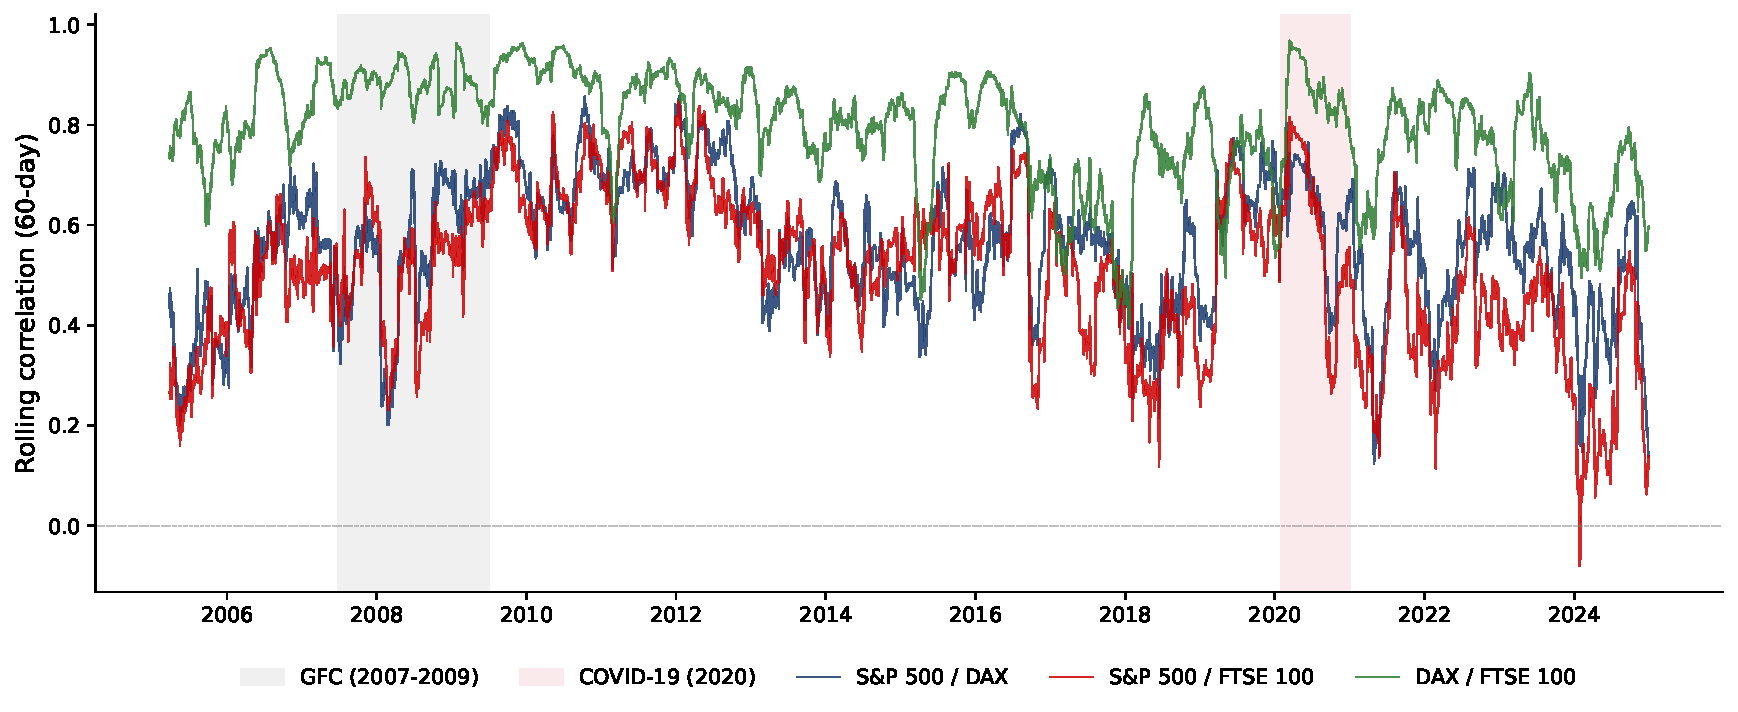
\includegraphics[width=0.95\textwidth, height=0.72\textheight, keepaspectratio]{../../charts/ch5b_rolling_correlations.pdf}
        \end{center}
    \end{cminipage}
    \hfill\quantlet{TSA\_ch5b\_rolling\_corr}{https://github.com/QuantLet/TSA/tree/main/TSA\_ch5b/TSA\_ch5b\_rolling\_corr}
\end{frame}

\begin{frame}{Distribuția corelațiilor: regimuri de criză vs.\ calm}
    \begin{cminipage}{0.95\textwidth}
    \vspace{-2mm}
        \begin{center}
            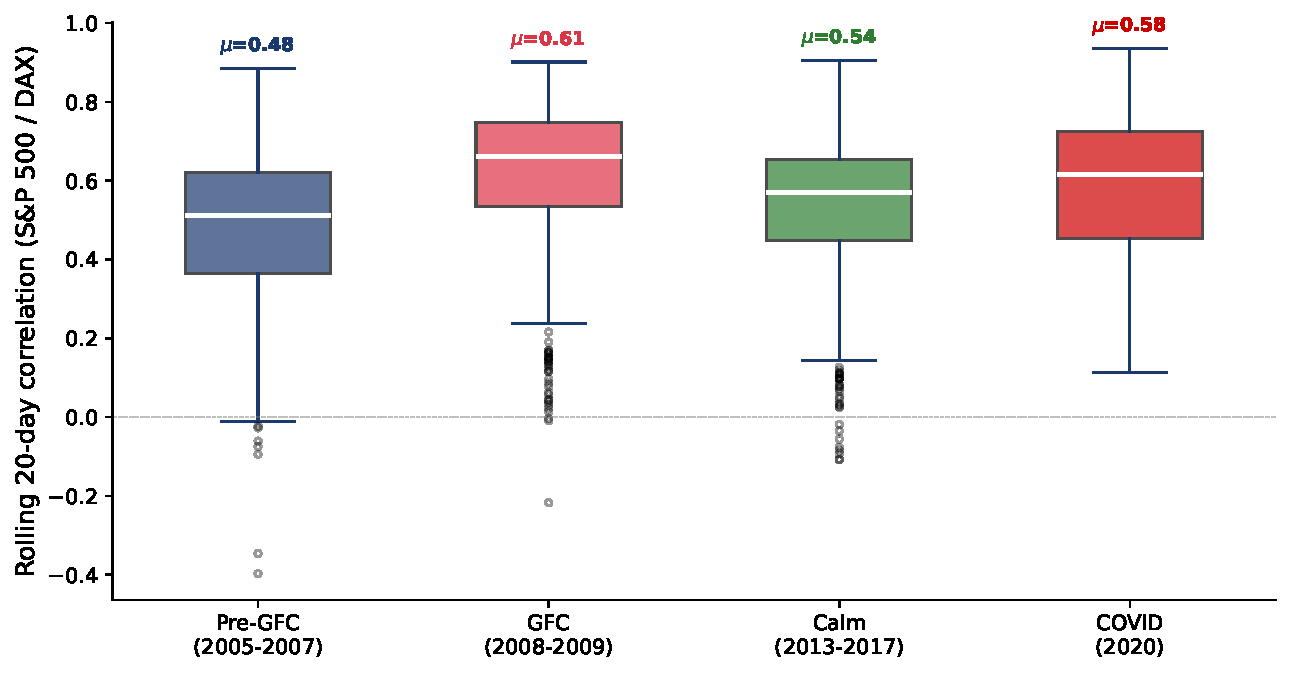
\includegraphics[width=0.85\textwidth, height=0.62\textheight, keepaspectratio]{../../charts/ch5b_crisis_boxplot.pdf}
        \end{center}
    \vspace{-2mm}
    {\footnotesize
    \begin{alertblock}{Observații cheie}
        \begin{itemize}\setlength{\itemsep}{0pt}
            \item Mediana corelației crește semnificativ în perioade de criză (GFC --- \textit{Global Financial Crisis}, COVID)
            \item Dispersia corelațiilor crește --- mai multă incertitudine în relațiile între piețe
        \end{itemize}
    \end{alertblock}
    }
    \end{cminipage}
    \hfill\quantlet{TSA\_ch5b\_crisis\_boxplot}{https://github.com/QuantLet/TSA/tree/main/TSA\_ch5b/TSA\_ch5b\_crisis\_boxplot}
\end{frame}

%=============================================================================
% SECȚIUNEA 2: CADRUL GARCH MULTIVARIAT
%=============================================================================
\section{Cadrul GARCH multivariat}

\begin{frame}{Formularea generală}
    \begin{cminipage}{0.95\textwidth}
    {\footnotesize
    \begin{block}{Procesul multivariat de randamente}
        \begin{itemize}\setlength{\itemsep}{0pt}
            \item Fie $\mathbf{r}_t = (r_{1t}, \ldots, r_{Nt})'$ un vector $N$-dimensional de randamente:
            \begin{align}
                \mathbf{r}_t &= \boldsymbol{\mu}_t + \boldsymbol{\varepsilon}_t \\
                \boldsymbol{\varepsilon}_t &= \mathbf{H}_t^{1/2} \mathbf{z}_t, \qquad \mathbf{z}_t \overset{iid}{\sim} \mathcal{N}(\mathbf{0}, \mathbf{I}_N)
            \end{align}
            \item $\boldsymbol{\mu}_t$ = vectorul mediei condiționale (adesea un VAR sau o constantă)
            \item $\mathbf{H}_t = \text{Var}(\boldsymbol{\varepsilon}_t \mid \mathcal{F}_{t-1})$ = matricea de covarianță condițională $N \times N$
            \item $\mathbf{H}_t^{1/2}$ = orice rădăcină pătratică a.î.\ $\mathbf{H}_t^{1/2}(\mathbf{H}_t^{1/2})' = \mathbf{H}_t$
        \end{itemize}
        \textit{Intuiție: $\mathbf{H}_t^{1/2}\mathbf{z}_t$ transformă șocuri independente în randamente corelate --- ``rădăcina pătrată'' imprimă structura de dependență.}
    \end{block}
    \begin{alertblock}{Provocarea dimensionalității (\textit{curse of dimensionality})}
        \begin{itemize}\setlength{\itemsep}{0pt}
            \item $\mathbf{H}_t$ are $N(N+1)/2$ elemente unice
            \item Pentru $N=50$ active: \textbf{1.275 de parametri variabili în timp} la fiecare $t$
        \end{itemize}
    \end{alertblock}
    }
    \end{cminipage}
\end{frame}

\begin{frame}{Semi-vectorizarea --- operatorul $\text{vech}(\cdot)$ (\textit{half-vectorization})}
    \begin{cminipage}{0.95\textwidth}
    \vspace{-3mm}
    {\footnotesize
    \begin{block}{Definiție}
        \begin{itemize}\setlength{\itemsep}{0pt}
            \item Operatorul $\text{vech}: \mathbb{R}^{N \times N} \to \mathbb{R}^{N^*}$ stochează \textbf{coloană cu coloană} elementele de pe și sub diagonala principală a unei matrice simetrice
            \item Dimensiunea vectorului rezultat: $N^* = N(N+1)/2$
            \item Matricea $\mathbf{H}_t$ este \textbf{simetrică}: $h_{ij,t} = h_{ji,t}$ --- $\text{vech}$ elimină cele $N(N-1)/2$ elemente redundante
        \end{itemize}
        \[
            \mathbf{H}_t = \begin{pmatrix} h_{11,t} & \textcolor{MediumGray}{h_{12,t}} & \textcolor{MediumGray}{h_{13,t}} \\ h_{12,t} & h_{22,t} & \textcolor{MediumGray}{h_{23,t}} \\ h_{13,t} & h_{23,t} & h_{33,t} \end{pmatrix} \xrightarrow{\text{vech}} \begin{pmatrix} h_{11,t} \\ h_{12,t} \\ h_{13,t} \\ h_{22,t} \\ h_{23,t} \\ h_{33,t} \end{pmatrix}
        \]
        \vspace{-2mm}
        {\small Elementele \textcolor{MediumGray}{gri} sunt duplicate --- $\text{vech}$ le elimină.}
    \end{block}
    \begin{alertblock}{Rol central în GARCH multivariat}
        \begin{itemize}\setlength{\itemsep}{0pt}
            \item Permite scrierea modelului ca ecuație vectorială: $\text{vech}(\mathbf{H}_t) = \mathbf{c} + \mathbf{A}\,\text{vech}(\boldsymbol{\varepsilon}_{t-1}\boldsymbol{\varepsilon}_{t-1}') + \mathbf{B}\,\text{vech}(\mathbf{H}_{t-1})$
            \item Dimensiune: $N^*\!=\!N(N\!+\!1)/2$ --- pentru $N\!=\!2$: 3 elemente; $N\!=\!10$: 55; $N\!=\!100$: 5.050
        \end{itemize}
    \end{alertblock}
    }
    \end{cminipage}
\end{frame}

\begin{frame}{Cerința de pozitiv-definire}
    \begin{cminipage}{0.95\textwidth}
    {\footnotesize
    \begin{block}{De ce contează pozitiv-definirea}
        \begin{itemize}\setlength{\itemsep}{0pt}
            \item Matricea $\mathbf{H}_t$ trebuie să fie \textbf{pozitiv definită} (p.d.) $\forall t$:
                \begin{itemize}\setlength{\itemsep}{0pt}
                    \item Varianța portofoliului: $\sigma_p^2 = \mathbf{w}'\mathbf{H}_t\mathbf{w} > 0$ pentru orice $\mathbf{w} \neq \mathbf{0}$
                    \item Log-verosimilitatea implică $\log|\mathbf{H}_t|$ și $\mathbf{H}_t^{-1}$ --- ambele necesită p.d.
                    \item Descompunerea Cholesky pentru simulare necesită p.d.
                \end{itemize}
        \end{itemize}
    \end{block}
    \begin{block}{Strategii pentru asigurarea pozitiv-definirii}
        \begin{enumerate}\setlength{\itemsep}{0pt}
            \item \textbf{Restricționarea parametrilor} a.î.\ $\mathbf{H}_t$ p.d.\ prin construcție (BEKK)
            \item \textbf{Descompunerea} $\mathbf{H}_t = \mathbf{D}_t \mathbf{R}_t \mathbf{D}_t$ și modelarea separată (DCC)
            \item \textbf{Spațiul factorilor} pentru reducerea dimensionalității (Factor GARCH, GO-GARCH)
        \end{enumerate}
    \end{block}
    }
    \end{cminipage}
\end{frame}

\begin{frame}{Descompunerea Cholesky (\textit{Cholesky Decomposition})}
    \begin{cminipage}{0.95\textwidth}
    \vspace{-2mm}
    {\scriptsize
    \begin{block}{Definiție}
        \begin{itemize}\setlength{\itemsep}{0pt}
            \item Orice matrice \textbf{simetrică pozitiv definită} $\mathbf{H}$ ($N \times N$) admite o \textbf{factorizare unică}: $\mathbf{H} = \mathbf{L}\mathbf{L}'$
            \item $\mathbf{L}$ este o matrice \textbf{inferior triunghiulară} cu elemente diagonale \textbf{strict pozitive}
            \item Complexitate: $O(N^3/3)$ --- de \textbf{două ori mai rapidă} decât inversarea directă
        \end{itemize}
    \end{block}
    \vspace{-1mm}
    \begin{block}{Exemplu: cazul $2 \times 2$}
        \begin{itemize}\setlength{\itemsep}{0pt}
            \item Fie $\mathbf{H} = \begin{pmatrix} h_{11} & h_{12} \\ h_{12} & h_{22} \end{pmatrix}$. Atunci $\mathbf{L} = \begin{pmatrix} \sqrt{h_{11}} & 0 \\ h_{12}/\sqrt{h_{11}} & \sqrt{h_{22} - h_{12}^2/h_{11}} \end{pmatrix}$
        \end{itemize}
    \end{block}
    \vspace{-1mm}
    \begin{alertblock}{Rolul în GARCH multivariat}
        \begin{itemize}\setlength{\itemsep}{0pt}
            \item \textbf{Simulare}: $\boldsymbol{\varepsilon}_t = \mathbf{L}_t \mathbf{z}_t$, unde $\mathbf{z}_t \sim N(\mathbf{0}, \mathbf{I})$ --- generează șocuri corelate
            \item \textbf{Log-verosimilitate}: $\log|\mathbf{H}_t| = 2\sum_i \log L_{ii}$ --- evită calculul direct al determinantului
            \item \textbf{Inversare}: rezolvă $\mathbf{L}_t \mathbf{x} = \boldsymbol{\varepsilon}_t$ prin substituție directă ($O(N^2)$ vs.\ $O(N^3)$)
        \end{itemize}
    \end{alertblock}
    }
    \end{cminipage}
\end{frame}

\begin{frame}{Proliferarea parametrilor: \textit{curse of dimensionality}}
    \begin{cminipage}{0.95\textwidth}
    {\footnotesize
    \begin{block}{Numărul de parametri pe model}
        \vspace{0.1cm}
        \begin{center}
        \begin{tabular}{lcc}
            \hline
            \textbf{Model} & \textbf{Parametri} & \textbf{$N=5$} \\
            \hline
            VEC(1,1) & $N(N+1)/2 + 2[N(N+1)/2]^2$ & 465 \\
            VEC Diagonal(1,1) & $3 \times N(N+1)/2$ & 45 \\
            BEKK(1,1) & $N(N+1)/2 + 2N^2$ & 65 \\
            BEKK Diagonal(1,1) & $N(N+1)/2 + 2N$ & 25 \\
            CCC(1,1) & $3N + N(N-1)/2$ & 25 \\
            DCC(1,1) & $3N + N(N-1)/2 + 2$ & 27 \\
            \hline
        \end{tabular}
        \end{center}
    \end{block}
    \begin{alertblock}{Implicație practică}
        \begin{itemize}\setlength{\itemsep}{0pt}
            \item Pentru $N$ mare, doar modelele \textbf{puternic \textit{parsimonious}} (CCC, DCC, BEKK scalar) sunt fezabile
            \item VEC/BEKK complet devin intractabile computațional pentru $N > 5$
        \end{itemize}
    \end{alertblock}
    }
    \end{cminipage}
\end{frame}

\begin{frame}{\textit{Curse of dimensionality}: vizualizare}
    \begin{cminipage}{0.95\textwidth}
        \begin{center}
            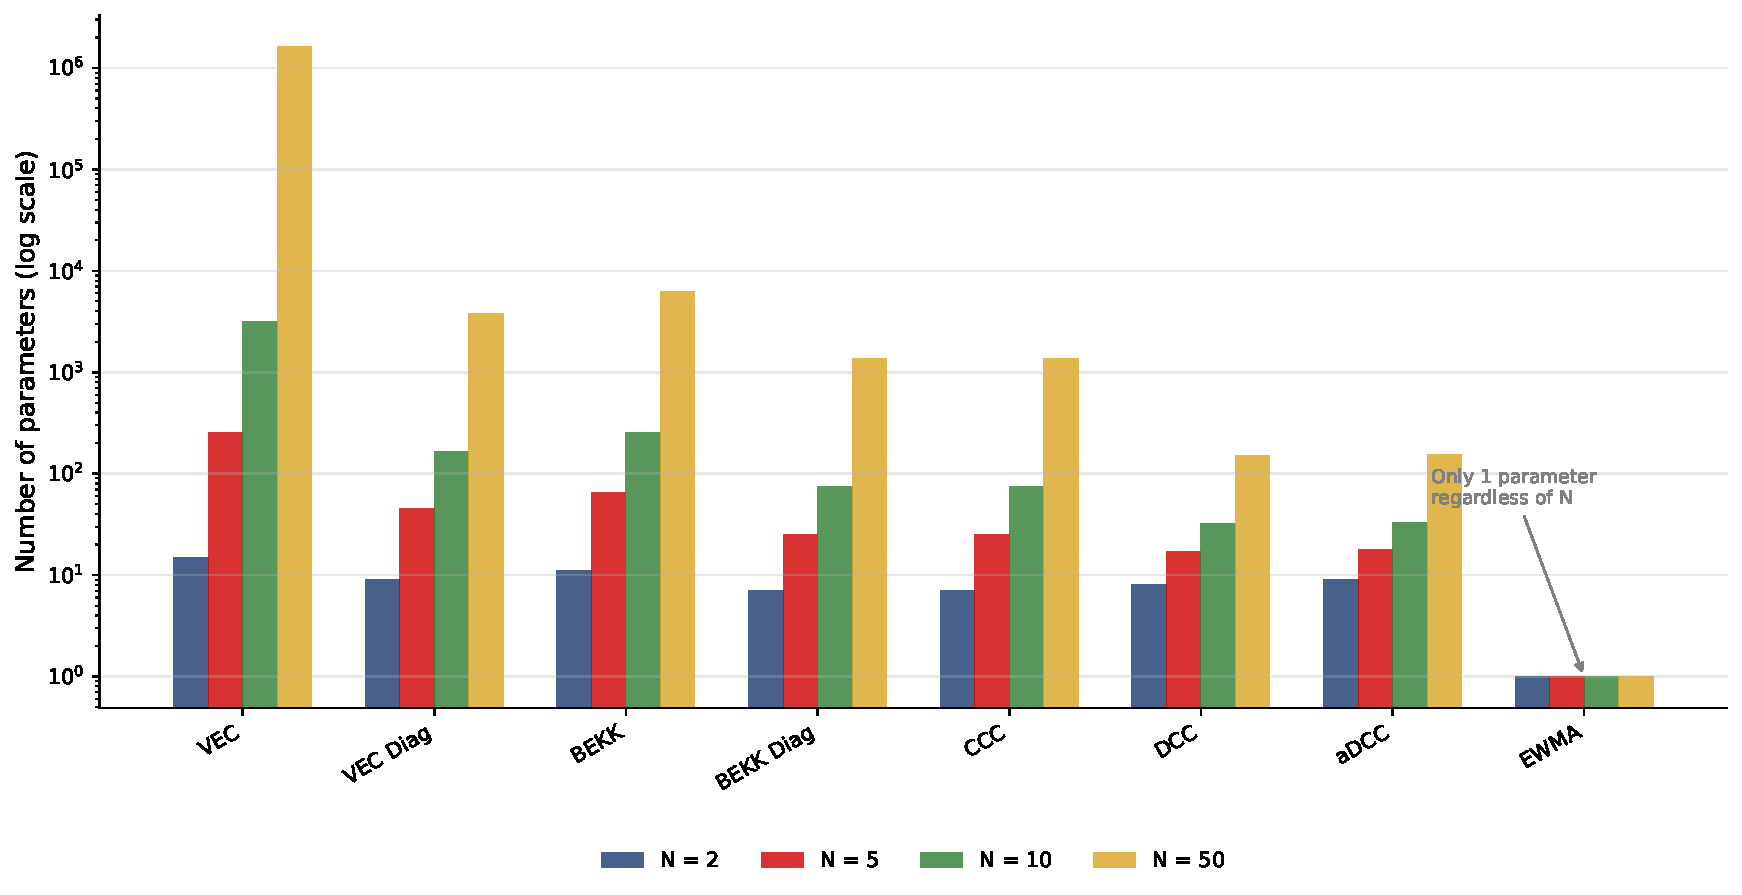
\includegraphics[width=0.92\textwidth, height=0.72\textheight, keepaspectratio]{../../charts/ch5b_param_comparison.pdf}
        \end{center}
    \end{cminipage}
    \hfill\quantlet{TSA\_ch5b\_param\_comparison}{https://github.com/QuantLet/TSA/tree/main/TSA\_ch5b/TSA\_ch5b\_param\_comparison}
\end{frame}

\begin{frame}{Log-verosimilitatea normală multivariată}
    \begin{cminipage}{0.95\textwidth}
    {\footnotesize
    \begin{block}{Log-verosimilitatea generală}
        \begin{itemize}\setlength{\itemsep}{0pt}
            \item Pentru $T$ observații de randamente $N$-dimensionale:
        \end{itemize}
        \[
            \mathcal{L}(\boldsymbol{\theta}) = -\frac{TN}{2}\log(2\pi) - \frac{1}{2}\sum_{t=1}^T \left[ \underbrace{\log|\mathbf{H}_t|}_{\text{penalizare volum}} + \underbrace{\boldsymbol{\varepsilon}_t'\mathbf{H}_t^{-1}\boldsymbol{\varepsilon}_t}_{\text{distanța Mahalanobis}} \right]
        \]
        \textit{Intuiție: verosimilitatea penalizează atât covarianța mare (``prognoză difuză'') cât și reziduurile standardizate mari (``prognoză proastă'').}
    \end{block}
    \begin{block}{Provocări computaționale}
        \begin{itemize}\setlength{\itemsep}{0pt}
            \item La fiecare $t$: calculează $\mathbf{H}_t$ ($O(N^2)$), inversa ($O(N^3)$) și determinantul ($O(N^3)$)
            \item \textbf{Truc Cholesky}: dacă $\mathbf{H}_t = \mathbf{L}_t\mathbf{L}_t'$:
                \begin{itemize}\setlength{\itemsep}{0pt}
                    \item $\log|\mathbf{H}_t| = 2\sum_{i}\log L_{ii}$
                    \item Rezolvă $\mathbf{L}_t\mathbf{x} = \boldsymbol{\varepsilon}_t$ prin substituție directă
                \end{itemize}
            \item Pentru DCC: estimarea în două etape reduce dramatic costul
        \end{itemize}
    \end{block}
    }
    \end{cminipage}
\end{frame}

%=============================================================================
% SECȚIUNEA 3: VEC ȘI VEC DIAGONAL
%=============================================================================
\section{Modele VEC și VEC Diagonal}

\begin{frame}{Modelul VEC --- \textit{VECtorized} (Bollerslev, Engle \& Wooldridge, 1988)}
    \begin{cminipage}{0.95\textwidth}
    {\footnotesize
    \begin{block}{Definiție}
        \begin{itemize}\setlength{\itemsep}{0pt}
            \item \textbf{VEC} = \textit{VECtorized} --- denumire derivată din operatorul $\text{vech}(\cdot)$ (semi-vectorizare). Modelul VEC(1,1):
        \end{itemize}
        \[
            \text{vech}(\mathbf{H}_t) = \underbrace{\mathbf{c}}_{\text{interceptare}} + \underbrace{\mathbf{A}\,\text{vech}(\boldsymbol{\varepsilon}_{t-1}\boldsymbol{\varepsilon}_{t-1}')}_{\text{impactul șocurilor}} + \underbrace{\mathbf{B}\,\text{vech}(\mathbf{H}_{t-1})}_{\text{persistență}}
        \]
        \begin{itemize}\setlength{\itemsep}{0pt}
            \item unde $\mathbf{c}$: vector $N^* \times 1$; $\mathbf{A}$, $\mathbf{B}$: matrice $N^* \times N^*$; $N^* = N(N+1)/2$
        \end{itemize}
        \textit{Intuiție: covarianța de azi = nivel de bază + șocurile de ieri + covarianța de ieri. $\mathbf{A}$ complet permite oricărui șoc să afecteze orice element de covarianță.}
    \end{block}
    \begin{alertblock}{Probleme}
        \begin{itemize}\setlength{\itemsep}{0pt}
            \item Pentru $N=3$: $N^*=6$, deci $\mathbf{A}$ și $\mathbf{B}$ sunt matrice $6 \times 6$ $\Rightarrow$ \textbf{78 parametri}
            \item \textbf{Nicio garanție} că $\mathbf{H}_t$ este pozitiv definită
            \item Condițiile pentru p.d.\ sunt complexe și greu de impus la estimare
        \end{itemize}
    \end{alertblock}
    }
    \end{cminipage}
\end{frame}

\begin{frame}{Produsul Hadamard (\textit{Hadamard Product})}
    \begin{cminipage}{0.95\textwidth}
    {\footnotesize
    \begin{block}{Definiție}
        \begin{itemize}\setlength{\itemsep}{0pt}
            \item Fie $\mathbf{A}, \mathbf{B} \in \mathbb{R}^{m \times n}$. \textbf{Produsul Hadamard} $\mathbf{A} \odot \mathbf{B}$ este multiplicarea \textbf{element cu element}:
            \[
                (\mathbf{A} \odot \mathbf{B})_{ij} = a_{ij} \cdot b_{ij}
            \]
            \item Matricele trebuie să aibă \textbf{aceeași dimensiune} --- rezultatul păstrează dimensiunea $m \times n$
        \end{itemize}
    \end{block}
    \begin{block}{Exemplu: cazul $2 \times 2$}
        \[
            \begin{pmatrix} 1 & 2 \\ 3 & 4 \end{pmatrix} \odot \begin{pmatrix} 5 & 6 \\ 7 & 8 \end{pmatrix} = \begin{pmatrix} 1 \cdot 5 & 2 \cdot 6 \\ 3 \cdot 7 & 4 \cdot 8 \end{pmatrix} = \begin{pmatrix} 5 & 12 \\ 21 & 32 \end{pmatrix}
        \]
    \end{block}
    \begin{alertblock}{Rolul în GARCH multivariat}
        \begin{itemize}\setlength{\itemsep}{0pt}
            \item VEC Diagonal: $\text{vech}(\mathbf{H}_t) = \mathbf{c} + \mathbf{a} \odot \text{vech}(\boldsymbol{\varepsilon}_{t-1}\boldsymbol{\varepsilon}_{t-1}') + \mathbf{b} \odot \text{vech}(\mathbf{H}_{t-1})$
            \item Fiecare element al lui $\mathbf{H}_t$ primește \textbf{proprii coeficienți} $a_k, b_k$ --- fără interacțiuni încrucișate
            \item Reduce parametrii de la $N^{*2}$ (VEC complet) la $3N^*$ (VEC Diagonal)
        \end{itemize}
    \end{alertblock}
    }
    \end{cminipage}
\end{frame}

\begin{frame}{Modelul VEC Diagonal}
    \begin{cminipage}{0.95\textwidth}
    \vspace{-3mm}
    {\scriptsize
    \begin{block}{Definiție (Bollerslev, Engle \& Wooldridge, 1988)}
        \begin{itemize}\setlength{\itemsep}{0pt}
            \item Se restricționează $\mathbf{A}$ și $\mathbf{B}$ să fie \textbf{diagonale}: $\text{vech}(\mathbf{H}_t) = \mathbf{c} + \mathbf{a} \odot \text{vech}(\boldsymbol{\varepsilon}_{t-1}\boldsymbol{\varepsilon}_{t-1}') + \mathbf{b} \odot \text{vech}(\mathbf{H}_{t-1})$
            \item $\odot$ = produsul Hadamard; $\mathbf{a}, \mathbf{b}$: vectori $N^* \times 1$
        \end{itemize}
    \end{block}
    \vspace{-1mm}
    \begin{block}{Element cu element pentru $N=2$}
        \vspace{-1mm}
        \begin{align}
            h_{11,t} &= c_{11} + a_{11}\,\varepsilon_{1,t-1}^2 + b_{11}\,h_{11,t-1} \\
            h_{12,t} &= c_{12} + a_{12}\,\varepsilon_{1,t-1}\varepsilon_{2,t-1} + b_{12}\,h_{12,t-1} \\
            h_{22,t} &= c_{22} + a_{22}\,\varepsilon_{2,t-1}^2 + b_{22}\,h_{22,t-1}
        \end{align}
        \vspace{-3mm}
        \textit{Intuiție: fiecare varianță/covarianță urmează propriul GARCH --- șocul activului 2 nu poate afecta varianța activului 1.}
    \end{block}
    \vspace{-1mm}
    \begin{alertblock}{Compromis}
        \begin{itemize}\setlength{\itemsep}{0pt}
            \item $3N^*$ parametri (gestionabil), dar fiecare element evoluează \textbf{independent} --- fără propagare între active
        \end{itemize}
    \end{alertblock}
    }
    \end{cminipage}
\end{frame}

\begin{frame}{VEC: exemplu bivariat}
    \begin{cminipage}{0.95\textwidth}
    {\footnotesize
    \begin{exampleblock}{Exemplu: două active ($N=2$)}
        \begin{itemize}\setlength{\itemsep}{0pt}
            \item Cu modelul VEC complet, $N^* = 3$:
            \[
                \begin{pmatrix} h_{11,t} \\ h_{12,t} \\ h_{22,t} \end{pmatrix} = \begin{pmatrix} c_1 \\ c_2 \\ c_3 \end{pmatrix} + \begin{pmatrix} a_{11} & a_{12} & a_{13} \\ a_{21} & a_{22} & a_{23} \\ a_{31} & a_{32} & a_{33} \end{pmatrix} \begin{pmatrix} \varepsilon_{1,t-1}^2 \\ \varepsilon_{1,t-1}\varepsilon_{2,t-1} \\ \varepsilon_{2,t-1}^2 \end{pmatrix} + \mathbf{B} \begin{pmatrix} h_{11,t-1} \\ h_{12,t-1} \\ h_{22,t-1} \end{pmatrix}
            \]
        \end{itemize}
    \end{exampleblock}
    \begin{block}{Interpretare}
        \begin{itemize}\setlength{\itemsep}{0pt}
            \item Elementele off-diagonal ale lui $\mathbf{A}$ captează \textbf{propagarea șocurilor între active}
                \begin{itemize}\setlength{\itemsep}{0pt}
                    \item $a_{13}$: impactul șocului activului 2 asupra varianței activului 1
                \end{itemize}
            \item Elementele off-diagonal ale lui $\mathbf{B}$ captează \textbf{propagarea persistenței volatilității}
            \item Total parametri: $3 + 9 + 9 = 21$ (doar pentru 2 active!)
        \end{itemize}
    \end{block}
    }
    \end{cminipage}
\end{frame}

\begin{frame}{VEC: perspectivă cheie și capcane frecvente}
    \begin{cminipage}{0.95\textwidth}
    \vspace{-2mm}
    {\scriptsize
    \begin{block}{\textcolor{MainBlue}{$\blacktriangleright$ Perspectivă cheie}: VEC este ``mama'' tuturor modelelor MGARCH}
        \begin{itemize}\setlength{\itemsep}{0pt}
            \item Fiecare model GARCH multivariat (BEKK, CCC, DCC) este o \textbf{versiune restricționată} a VEC
            \item Ecuația VEC este cea mai generală dinamică liniară pentru $\mathbf{H}_t$
            \item Toate restricțiile de aici sunt alegeri despre care parametri se elimină
        \end{itemize}
    \end{block}
    \vspace{-2mm}
    \begin{alertblock}{\textcolor{Crimson}{$\blacktriangleright$ Capcană frecventă}: confuzia între VEC și VEC Diagonal}
        \begin{itemize}\setlength{\itemsep}{0pt}
            \item VEC Diagonal ($\mathbf{A}, \mathbf{B}$ diagonale) elimină \textit{toate efectele încrucișate}
            \item Fiecare $h_{ij,t}$ depinde doar de propriul lag și de $\varepsilon_{i,t-1}\varepsilon_{j,t-1}$
            \item \textbf{Nu înseamnă} doar ``mai puțini parametri'': elimină fundamental propagarea volatilității
        \end{itemize}
    \end{alertblock}
    \vspace{-2mm}
    \begin{exampleblock}{\textcolor{Forest}{$\blacktriangleright$ Când NU se folosește VEC}}
        \begin{itemize}\setlength{\itemsep}{0pt}
            \item \textbf{Niciodată} VEC complet pentru $N > 2$ --- $O(N^4)$ parametri, estimarea diverge
            \item \textbf{Evitați} VEC Diagonal când spillovers contează (ex.: studii de contagiune bancară)
            \item \textbf{Săriți} peste VEC dacă aveți nevoie doar de varianța portofoliului --- CCC/DCC sunt mai rapide și garantat p.d.
        \end{itemize}
    \end{exampleblock}
    }
    \end{cminipage}
\end{frame}

\begin{frame}{Rezumatul secțiunii VEC}
    \begin{cminipage}{0.95\textwidth}
    {\footnotesize
    \begin{block}{3 lucruri de reținut}
        \begin{enumerate}\setlength{\itemsep}{2pt}
            \item VEC este cel mai \textbf{general} model MGARCH liniar --- toate celelalte modele îl restricționează
            \item VEC Diagonal este estimabil dar elimină propagarea; VEC complet este bogat dar neestimabil pentru $N > 2$
            \item Problema centrală nerezolvată: \textbf{nicio garanție de pozitiv-definire}
        \end{enumerate}
    \end{block}
    \begin{alertblock}{Poziționarea modelului}
        \begin{itemize}\setlength{\itemsep}{0pt}
            \item \textbf{Utilizare}: $N = 2$ și necesitate de flexibilitate maximă
            \item \textbf{vs.\ BEKK}: BEKK garantează p.d.\ cu aceeași expresivitate --- preferați BEKK
        \end{itemize}
    \end{alertblock}
    }
    \end{cminipage}
\end{frame}

%=============================================================================
% TRANZIȚIE: VEC → BEKK
%=============================================================================

\begin{frame}{De la VEC la BEKK: ce nu a funcționat?}
    \begin{cminipage}{0.95\textwidth}
    {\footnotesize
    \textit{\textbf{O propoziție:} VEC este cel mai general model, dar nu garantează matrici pozitiv definite.}
    \vspace{0.2cm}
    \begin{block}{Ce nu a funcționat la VEC?}
        \begin{itemize}\setlength{\itemsep}{2pt}
            \item VEC este cel mai \textbf{general} GARCH multivariat --- fiecare element al lui $\mathbf{H}_t$ are dinamica proprie
            \item Dar: (1) \textbf{nicio garanție} că $\mathbf{H}_t$ este pozitiv definită, (2) parametrii \textbf{explodează} ($O(N^4)$)
            \item VEC Diagonal rezolvă (2) dar eșuează la (1) --- și pierde efectele de spillover
        \end{itemize}
    \end{block}
    \vspace{0.1cm}
    \begin{alertblock}{Problema fundamentală}
        \begin{itemize}\setlength{\itemsep}{0pt}
            \item VEC scrie $\text{vech}(\mathbf{H}_t) = \mathbf{c} + \mathbf{A}\,\text{vech}(\boldsymbol{\varepsilon}_{t-1}\boldsymbol{\varepsilon}_{t-1}') + \mathbf{B}\,\text{vech}(\mathbf{H}_{t-1})$
            \item Nimic din această ecuație \textbf{nu forțează} $\mathbf{H}_t$ să fie p.d.\ la fiecare $t$
        \end{itemize}
    \end{alertblock}
    }
    \end{cminipage}
\end{frame}

\begin{frame}{Intuiția BEKK: construiește PD în structură}
    \begin{cminipage}{0.95\textwidth}
    {\footnotesize
    \textit{\textbf{O propoziție:} BEKK garantează pozitiv-definirea prin forma pătratică $\mathbf{A}'\mathbf{M}\mathbf{A}$.}
    \vspace{0.2cm}
    \begin{block}{Soluția BEKK}
        \begin{itemize}\setlength{\itemsep}{2pt}
            \item Scrie $\mathbf{H}_t = \mathbf{C}\mathbf{C}' + \mathbf{A}'\boldsymbol{\varepsilon}_{t-1}\boldsymbol{\varepsilon}_{t-1}'\mathbf{A} + \mathbf{B}'\mathbf{H}_{t-1}\mathbf{B}$
            \item Fiecare termen este p.s.d.\ \textbf{prin construcție} ($\mathbf{X}'\mathbf{M}\mathbf{X} \succeq 0$ pentru orice $\mathbf{M} \succeq 0$)
            \item Suma de matrice p.s.d.\ + o matrice p.d.\ = p.d.\ întotdeauna
        \end{itemize}
    \end{block}
    \vspace{0.1cm}
    \begin{alertblock}{Prețul plătit}
        \begin{itemize}\setlength{\itemsep}{0pt}
            \item $2N^2 + N(N+1)/2$ parametri --- pentru $N = 10$: \textbf{255 parametri}
            \item Estimare numerică instabilă cu optima locale multiple
        \end{itemize}
    \end{alertblock}
    }
    \end{cminipage}
\end{frame}

%=============================================================================
% SECȚIUNEA 4: MODELUL BEKK
%=============================================================================
\section{Modelul BEKK}

\begin{frame}{Modelul BEKK (Engle \& Kroner, 1995)}
    \begin{cminipage}{0.95\textwidth}
    \vspace{-2mm}
    {\scriptsize
    \begin{block}{Definiție: BEKK(1,1)}
        \[
            \mathbf{H}_t = \underbrace{\mathbf{C}\mathbf{C}'}_{\text{interceptare (p.d.)}} + \underbrace{\mathbf{A}'\boldsymbol{\varepsilon}_{t-1}\boldsymbol{\varepsilon}_{t-1}'\mathbf{A}}_{\text{impactul șocurilor (p.s.d.)}} + \underbrace{\mathbf{B}'\mathbf{H}_{t-1}\mathbf{B}}_{\text{persistență (p.s.d.)}}
        \]
        \begin{itemize}\setlength{\itemsep}{0pt}
            \item $\mathbf{C}$: $N \times N$ inferior triunghiulară; $\mathbf{A}, \mathbf{B}$: matrice $N \times N$
        \end{itemize}
        \textit{Intuiție: forma pătratică $\mathbf{A}'\mathbf{M}\mathbf{A}$ este întotdeauna p.s.d. --- pozitiv-definirea vine ``gratuit.''}
    \end{block}
    \vspace{-1mm}
    \begin{block}{Proprietăți cheie}
        \begin{itemize}\setlength{\itemsep}{0pt}
            \item $\mathbf{H}_t$ este \textbf{pozitiv definită prin construcție} (dacă $\mathbf{C}\mathbf{C}'$ este p.d.)
                \begin{itemize}\setlength{\itemsep}{0pt}
                    \item $\mathbf{A}'\mathbf{M}\mathbf{A}$ este pozitiv semi-definită pentru orice matrice p.s.d.\ $\mathbf{M}$
                \end{itemize}
            \item Captează atât \textbf{persistența propriei volatilități} cât și \textbf{propagarea între active}
            \item Parametri: $N(N+1)/2 + 2N^2$ --- pentru $N=3$: $6 + 18 = 24$
        \end{itemize}
    \end{block}
    \vspace{-1mm}
    \textcolor{Crimson}{$\blacktriangleright$ \textbf{Avertisment practic}: BEKK nu scalează} --- $2N^2$ parametri $\Rightarrow$ intractabil pentru $N > 5$.
    BEKK: \textbf{B}aba, \textbf{E}ngle, \textbf{K}raft și \textbf{K}roner (1990, working paper).
    }
    \end{cminipage}
\end{frame}

\begin{frame}{BEKK: cazul bivariat}
    \begin{cminipage}{0.95\textwidth}
    {\scriptsize
    \begin{block}{Dezvoltarea BEKK(1,1) pentru $N=2$}
        \begin{itemize}\setlength{\itemsep}{0pt}
            \item Fie $\mathbf{A} = \begin{pmatrix} a_{11} & a_{12} \\ a_{21} & a_{22} \end{pmatrix}$, $\mathbf{B} = \begin{pmatrix} b_{11} & b_{12} \\ b_{21} & b_{22} \end{pmatrix}$, $\mathbf{C} = \begin{pmatrix} c_{11} & 0 \\ c_{21} & c_{22} \end{pmatrix}$
        \end{itemize}
        \begin{align}
            h_{11,t} &= c_{11}^2 + a_{11}^2\varepsilon_{1,t-1}^2 + 2a_{11}a_{21}\varepsilon_{1,t-1}\varepsilon_{2,t-1} + a_{21}^2\varepsilon_{2,t-1}^2 \\
            &\quad + b_{11}^2 h_{11,t-1} + 2b_{11}b_{21}h_{12,t-1} + b_{21}^2 h_{22,t-1} \nonumber \\[3pt]
            h_{12,t} &= c_{11}c_{21} + a_{11}a_{12}\varepsilon_{1,t-1}^2 + (a_{11}a_{22}+a_{12}a_{21})\varepsilon_{1,t-1}\varepsilon_{2,t-1} + a_{21}a_{22}\varepsilon_{2,t-1}^2 \\
            &\quad + b_{11}b_{12}h_{11,t-1} + (b_{11}b_{22}+b_{12}b_{21})h_{12,t-1} + b_{21}b_{22}h_{22,t-1} \nonumber
        \end{align}
    \end{block}
    \begin{alertblock}{Interpretarea spillover-ului}
        \begin{itemize}\setlength{\itemsep}{0pt}
            \item Termenul $a_{21}^2\varepsilon_{2,t-1}^2$ în $h_{11,t}$: șocul din activul 2 afectează varianța activului 1
            \item Aceasta este o \textbf{propagare de volatilitate} (spillover) --- specifică BEKK
        \end{itemize}
    \end{alertblock}
    }
    \end{cminipage}
\end{frame}

\begin{frame}{BEKK Diagonal și BEKK Scalar}
    \begin{cminipage}{0.95\textwidth}
    \vspace{-2mm}
    {\scriptsize
    \begin{block}{BEKK Diagonal}
        \begin{itemize}\setlength{\itemsep}{0pt}
            \item Se restricționează $\mathbf{A}$ și $\mathbf{B}$ să fie \textbf{diagonale}:
            \[
                \mathbf{H}_t = \mathbf{C}\mathbf{C}' + \text{diag}(\mathbf{a})'\boldsymbol{\varepsilon}_{t-1}\boldsymbol{\varepsilon}_{t-1}'\text{diag}(\mathbf{a}) + \text{diag}(\mathbf{b})'\mathbf{H}_{t-1}\text{diag}(\mathbf{b})
            \]
            \item Parametri: $N(N+1)/2 + 2N$. Element cu element: $h_{ij,t} = c_{ij}^* + a_i a_j \varepsilon_{i,t-1}\varepsilon_{j,t-1} + b_i b_j h_{ij,t-1}$
        \end{itemize}
    \end{block}
    \vspace{-1mm}
    \begin{block}{BEKK Scalar}
        \begin{itemize}\setlength{\itemsep}{0pt}
            \item Restricție suplimentară: $\mathbf{A} = a\mathbf{I}_N$, $\mathbf{B} = b\mathbf{I}_N$:
            \[
                \mathbf{H}_t = \mathbf{C}\mathbf{C}' + a^2\boldsymbol{\varepsilon}_{t-1}\boldsymbol{\varepsilon}_{t-1}' + b^2\mathbf{H}_{t-1}
            \]
            \item Parametri: $N(N+1)/2 + 2$ --- toate elementele au \textbf{aceeași dinamică}
        \end{itemize}
        \textit{Intuiție: BEKK scalar = ``un buton pentru sensibilitatea la șocuri, unul pentru memorie'' --- identic pentru toate perechile.}
    \end{block}
    \vspace{-1mm}
    \begin{alertblock}{Compromis}
        \begin{itemize}\setlength{\itemsep}{0pt}
            \item BEKK Diagonal/Scalar: fezabil pentru $N$ mare, dar \textbf{fără propagare între active}.
        \end{itemize}
    \end{alertblock}
    }
    \end{cminipage}
\end{frame}

\begin{frame}{Produsul Kronecker (\textit{Kronecker Product})}
    \begin{cminipage}{0.95\textwidth}
    \vspace{-3mm}
    {\scriptsize
    \begin{block}{Definiție}
        \begin{itemize}\setlength{\itemsep}{0pt}
            \item Fie $\mathbf{A} \in \mathbb{R}^{m \times n}$ și $\mathbf{B} \in \mathbb{R}^{p \times q}$. \textbf{Produsul Kronecker} $\mathbf{A} \otimes \mathbf{B}$ este matricea bloc $mp \times nq$:
            \vspace{-1mm}
            \[
                \mathbf{A} \otimes \mathbf{B} = \begin{pmatrix} a_{11}\mathbf{B} & \cdots & a_{1n}\mathbf{B} \\ \vdots & \ddots & \vdots \\ a_{m1}\mathbf{B} & \cdots & a_{mn}\mathbf{B} \end{pmatrix}
            \]
            \vspace{-3mm}
            \item Dimensiunile \textbf{nu} trebuie să fie egale (diferit de Hadamard)
        \end{itemize}
    \end{block}
    \vspace{-2mm}
    \begin{block}{Exemplu: $2 \times 2$}
        \begin{itemize}\setlength{\itemsep}{0pt}
            \item $\begin{pmatrix} a & b \\ c & d \end{pmatrix} \otimes \begin{pmatrix} e & f \\ g & h \end{pmatrix} = \begin{pmatrix} ae & af & be & bf \\ ag & ah & bg & bh \\ ce & cf & de & df \\ cg & ch & dg & dh \end{pmatrix}$ \quad (rezultat $4 \times 4$)
        \end{itemize}
    \end{block}
    \vspace{-2mm}
    \begin{alertblock}{Rolul în GARCH multivariat}
        \begin{itemize}\setlength{\itemsep}{0pt}
            \item Condiția de stationaritate BEKK: $\rho(\mathbf{A} \otimes \mathbf{A} + \mathbf{B} \otimes \mathbf{B}) < 1$
            \item Covarianța necondiționată: $\text{vech}(\bar{\mathbf{H}}) = (\mathbf{I} - \mathbf{A} \otimes \mathbf{A} - \mathbf{B} \otimes \mathbf{B})^{-1}\text{vech}(\mathbf{C}\mathbf{C}')$
        \end{itemize}
    \end{alertblock}
    }
    \end{cminipage}
\end{frame}

\begin{frame}{BEKK: stationaritate și covarianță necondiționată}
    \begin{cminipage}{0.95\textwidth}
    {\footnotesize
    \begin{block}{Condiția de stationaritate}
        \begin{itemize}\setlength{\itemsep}{0pt}
            \item Procesul BEKK(1,1) este staționar în covarianță dacă și numai dacă:
        \end{itemize}
        \[
            \rho(\mathbf{A} \otimes \mathbf{A} + \mathbf{B} \otimes \mathbf{B}) < 1
        \]
        \begin{itemize}\setlength{\itemsep}{0pt}
            \item unde $\rho(\cdot)$ denotă raza spectrală și $\otimes$ este produsul Kronecker
        \end{itemize}
        \textit{Intuiție: analogul multivariat al $\alpha + \beta < 1$ --- șocurile trebuie să se atenueze, nu să explodeze.}
    \end{block}
    \vspace{0.1cm}
    \begin{block}{Matricea de covarianță necondiționată}
        \begin{itemize}\setlength{\itemsep}{0pt}
            \item Dacă condiția de stationaritate este satisfăcută:
        \end{itemize}
        \[
            \text{vech}(\bar{\mathbf{H}}) = (\mathbf{I}_{N^*} - \mathbf{A} \otimes \mathbf{A} - \mathbf{B} \otimes \mathbf{B})^{-1} \text{vech}(\mathbf{C}\mathbf{C}')
        \]
        \textit{Intuiție: matricea de covarianță pe termen lung spre care gravitează $\mathbf{H}_t$ --- precum $\bar{\sigma}^2 = \omega/(1-\alpha-\beta)$ în GARCH univariat.}
    \end{block}
    }
    \end{cminipage}
\end{frame}

\begin{frame}{BEKK: avantaje, dezavantaje și alegerea variantei}
    \begin{cminipage}{0.95\textwidth}
    \vspace{-3mm}
    {\scriptsize
    \begin{block}{Avantaje ale BEKK}
        \begin{itemize}\setlength{\itemsep}{0pt}
            \item \textbf{Pozitiv-definire prin construcție} --- nu necesită restricții suplimentare
            \item Captează \textbf{volatility spillovers} --- singura clasă care le modelează direct
            \item Interpretare directă a matricelor $\mathbf{A}$ și $\mathbf{B}$: transmitere de șocuri și persistență
        \end{itemize}
    \end{block}
    \begin{alertblock}{Dezavantaje}
        \begin{itemize}\setlength{\itemsep}{0pt}
            \item \textbf{Explozie de parametri}: BEKK complet pentru $N=10$ $\Rightarrow$ 255 parametri
            \item Optimizare numerică \textbf{instabilă} --- multiple optima locale, convergență lentă
            \item Rezultatele pot fi \textbf{sensibile la valorile inițiale} ale algoritmului
            \item Nu se descompune în etape --- estimare simultană obligatorie
        \end{itemize}
    \end{alertblock}
    \begin{block}{Regulă practică}
        \begin{itemize}\setlength{\itemsep}{0pt}
            \item $N \leq 3$: BEKK complet (dacă spillovers sunt relevante)
            \item $3 < N \leq 10$: BEKK diagonal
            \item $N > 10$: treceți la DCC sau modele factoriale
        \end{itemize}
    \end{block}
    }
    \end{cminipage}
\end{frame}

%=============================================================================
% BEKK: PERSPECTIVĂ CHEIE + CAPCANE
%=============================================================================

\begin{frame}{BEKK: perspectivă cheie și capcane frecvente}
    \begin{cminipage}{0.95\textwidth}
    \vspace{-2mm}
    {\scriptsize
    \begin{block}{\textcolor{MainBlue}{$\blacktriangleright$ Perspectivă cheie}: BEKK este o ``reparametrizare inteligentă'' a VEC}
        \begin{itemize}\setlength{\itemsep}{0pt}
            \item BEKK nu adaugă economie nouă --- scrie \textit{aceeași} dinamică într-o formă în care p.d.\ este automată
            \item Forma pătratică $\mathbf{A}'\mathbf{M}\mathbf{A}$ este p.s.d.\ prin algebră liniară, nu prin teorie economică
            \item BEKK schimbă flexibilitate contra comoditate matematică
        \end{itemize}
    \end{block}
    \vspace{-2mm}
    \begin{alertblock}{\textcolor{Crimson}{$\blacktriangleright$ Capcană frecventă}: folosirea BEKK complet pentru $N > 5$}
        \begin{itemize}\setlength{\itemsep}{0pt}
            \item BEKK complet pentru $N = 10$: \textbf{255 parametri} --- optimizatorul găsește optima locale, rezultatele sunt fragile
            \item Caporin \& McAleer (2012): ``BEKK complet este esențial neinterpretabil pentru $N > 3$''
            \item BEKK diagonal este adesea alegerea practică, dar atunci spillovers dispar --- anulând scopul BEKK
        \end{itemize}
    \end{alertblock}
    \vspace{-2mm}
    \begin{exampleblock}{\textcolor{Forest}{$\blacktriangleright$ Când NU se folosește BEKK}}
        \begin{itemize}\setlength{\itemsep}{0pt}
            \item $N > 5$: folosiți DCC sau modele factoriale
            \item Când nu vă interesează \textit{direcția} spillover-urilor (DCC captează co-mișcarea fără canale de spillover)
            \item Când aveți nevoie de re-estimare rapidă (BEKK: ore vs.\ DCC: secunde pentru $N = 50$)
        \end{itemize}
    \end{exampleblock}
    }
    \end{cminipage}
\end{frame}

\begin{frame}{Rezumatul secțiunii BEKK}
    \begin{cminipage}{0.95\textwidth}
    {\footnotesize
    \begin{block}{3 lucruri de reținut}
        \begin{enumerate}\setlength{\itemsep}{2pt}
            \item BEKK garantează p.d.\ prin forma pătratică $\mathbf{A}'\mathbf{M}\mathbf{A}$ --- \textbf{singurul} model care captează direct propagarea
            \item BEKK complet: bogat dar infezabil pentru $N > 5$; BEKK diagonal: scalabil dar fără propagare
            \item Estimarea necesită optimizare simultană --- fără scurtătură în două etape
        \end{enumerate}
    \end{block}
    \begin{alertblock}{Poziționarea modelului}
        \begin{itemize}\setlength{\itemsep}{0pt}
            \item \textbf{Utilizare}: $N \leq 5$ și \textit{direcția} spillover-ului contează
            \item \textbf{vs.\ VEC}: aceeași flexibilitate, p.d.\ garantată \quad \textbf{vs.\ DCC}: DCC scalează mai bine dar nu identifică direcția spillover-ului
        \end{itemize}
    \end{alertblock}
    \vspace{1mm}
    \textit{\textbf{Concluzie cheie:} Folosiți BEKK când $N \leq 5$ și trebuie să știți \textbf{cine transmite volatilitate cui}.}
    }
    \end{cminipage}
\end{frame}

%=============================================================================
% TRANZIȚIE: BEKK → CCC
%=============================================================================

\begin{frame}{De la BEKK la CCC: descompunerea care a schimbat totul}
    \begin{cminipage}{0.95\textwidth}
    \vspace{-2mm}
    {\scriptsize
    \begin{block}{Ce ne-a învățat BEKK --- și unde eșuează}
        \begin{itemize}\setlength{\itemsep}{0pt}
            \item BEKK a \textbf{rezolvat} problema PD și modelează spillover-uri de volatilitate direct
            \item Dar: $N(N+1)/2 + 2N^2$ parametri $\Rightarrow$ estimarea se prăbușește pentru $N > 5$
            \item Estimare simultană a tuturor parametrilor --- fără descompunere în sub-probleme mai simple
            \item \textcolor{Crimson}{Practicienii au abandonat BEKK pentru portofolii mari la sfârșitul anilor 1990}
        \end{itemize}
    \end{block}
    \vspace{-2mm}
    \begin{alertblock}{Intuiția lui Bollerslev (1990): separă ce se schimbă de ce nu se schimbă}
        \begin{itemize}\setlength{\itemsep}{0pt}
            \item \textbf{Observație}: varianțele se schimbă zilnic, dar \textit{corelațiile} se mișcă lent
            \item \textbf{Idee}: descompune $\mathbf{H}_t = \mathbf{D}_t \mathbf{R} \mathbf{D}_t$ unde $\mathbf{D}_t$ variază dar $\mathbf{R}$ este fixat
            \item Aceasta separă o problemă \textbf{dificilă} simultană în $N$ probleme \textbf{ușoare} univariate + o estimare de corelație
        \end{itemize}
    \end{alertblock}
    \vspace{-2mm}
    \begin{exampleblock}{Compromisul (\textit{trade-off})}
        \begin{itemize}\setlength{\itemsep}{0pt}
            \item \textcolor{Forest}{Câștigat}: scalabilitate ($3N + N(N-1)/2$ param.), estimare în 2 etape, funcționează pt. $N > 100$
            \item \textcolor{Crimson}{Pierdut}: spillover-uri de volatilitate, corelații variabile în timp ($\mathbf{R}$ constant!)
            \item Acest compromis a motivat CCC --- și apoi DCC pentru a restabili corelațiile dinamice
        \end{itemize}
    \end{exampleblock}
    }
    \end{cminipage}
\end{frame}

%=============================================================================
% SECȚIUNEA 5: MODELUL CCC
%=============================================================================
\section{Corelația Condițională Constantă --- CCC (\textit{Constant Conditional Correlation})}

\begin{frame}{CCC: descompunerea $\mathbf{H}_t = \mathbf{D}_t \mathbf{R} \mathbf{D}_t$}
    \begin{cminipage}{0.95\textwidth}
    {\footnotesize
    \textit{\textbf{O propoziție:} Covarianțele se schimbă doar pentru că volatilitățile se schimbă --- ``cablajul'' între active rămâne fix.}
    \vspace{0.2cm}
    \begin{block}{Ideea cheie: separarea varianțelor de corelații}
        \begin{itemize}\setlength{\itemsep}{0pt}
            \item Se descompune matricea de covarianță condițională:
        \end{itemize}
        \[
            \mathbf{H}_t = \underbrace{\mathbf{D}_t}_{\text{volatilități}} \underbrace{\mathbf{R}}_{\text{corelații}} \underbrace{\mathbf{D}_t}_{\text{volatilități}}
        \]
        \begin{itemize}\setlength{\itemsep}{0pt}
            \item $\mathbf{D}_t = \text{diag}(\sqrt{h_{11,t}}, \ldots, \sqrt{h_{NN,t}})$ --- abatere standard condițională
            \item $\mathbf{R}$ --- matrice de corelație \textbf{constantă} (invariabilă în timp)
            \item Fiecare $h_{ii,t}$ urmează un \textbf{GARCH(1,1) univariat}:
                $h_{ii,t} = \omega_i + \alpha_i \varepsilon_{i,t-1}^2 + \beta_i h_{ii,t-1}$
        \end{itemize}
    \end{block}
    }
    \end{cminipage}
\end{frame}

\begin{frame}{CCC: proprietăți și număr de parametri}
    \begin{cminipage}{0.95\textwidth}
    {\footnotesize
    \textit{\textbf{O propoziție:} CCC reduce o problemă imensă de estimare la $N$ GARCH-uri univariate simple plus o matrice de corelație.}
    \vspace{0.2cm}
    \begin{block}{Proprietăți}
        \begin{itemize}\setlength{\itemsep}{2pt}
            \item $\mathbf{H}_t$ p.d.\ iff $\mathbf{R}$ p.d.\ și toți $h_{ii,t} > 0$
            \item Covarianțe: $h_{ij,t} = \rho_{ij}\sqrt{h_{ii,t}}\sqrt{h_{jj,t}}$
            \item Parametri: $3N$ (GARCH univariat) $+ N(N-1)/2$ (corelații)
        \end{itemize}
    \end{block}
    \vspace{0.1cm}
    \begin{alertblock}{Comparație}
        \begin{itemize}\setlength{\itemsep}{0pt}
            \item $N = 50$: CCC necesită \textbf{1.375} parametri vs.\ BEKK $\approx$ 6.275
            \item Estimare în două etape: fiecare etapă este de dimensiune redusă
        \end{itemize}
    \end{alertblock}
    \vspace{0.2cm}
    \textit{\textbf{Concluzie cheie:} CCC presupune corelații fixe --- covarianțele se schimbă doar pentru că volatilitățile se schimbă.}
    }
    \end{cminipage}
\end{frame}

\begin{frame}{CCC: estimare în două etape}
    \begin{cminipage}{0.95\textwidth}
    \vspace{-2mm}
    {\scriptsize
    \begin{block}{Etapa 1: estimare modele GARCH univariate}
        \begin{itemize}\setlength{\itemsep}{0pt}
            \item Pentru fiecare activ $i = 1, \ldots, N$:
                \begin{enumerate}\setlength{\itemsep}{0pt}
                    \item Se estimează un model GARCH(1,1) pentru $r_{it}$
                    \item Se obțin reziduurile standardizate: $z_{it} = \varepsilon_{it} / \sqrt{h_{ii,t}}$
                \end{enumerate}
        \end{itemize}
    \end{block}
    \vspace{-1mm}
    \begin{block}{Etapa 2: estimarea matricei de corelație}
        \begin{itemize}\setlength{\itemsep}{0pt}
            \item Corelația eșantionară a reziduurilor standardizate:
            $\hat{\mathbf{R}} = \frac{1}{T}\sum_{t=1}^T \mathbf{z}_t\mathbf{z}_t'$
        \end{itemize}
    \end{block}
    \vspace{-1mm}
    \begin{alertblock}{Avantaj}
        \begin{itemize}\setlength{\itemsep}{0pt}
            \item Fiecare etapă implică \textbf{optimizare de dimensiune redusă}: $N$ optimizări univariate (3 param.\ fiecare)
            \item Etapa 2: corelație eșantionară simplă --- fără optimizare numerică
        \end{itemize}
    \end{alertblock}
    }
    \end{cminipage}
\end{frame}

\begin{frame}{CCC: puncte forte și limitări}
    \begin{cminipage}{0.95\textwidth}
    {\footnotesize
    \begin{block}{Puncte forte}
        \begin{itemize}\setlength{\itemsep}{0pt}
            \item \textbf{Parcimonie}: puțini parametri, ușor de estimat chiar pentru $N$ mare
            \item \textbf{Pozitiv-definire}: garantată prin construcție
            \item \textbf{Interpretabilitate}: covarianțele variabile în timp sunt determinate doar de varianțe
            \item Bun \textbf{model de referință} pentru comparație
        \end{itemize}
    \end{block}
    \vspace{0.2cm}
    \begin{alertblock}{Limitări}
        \begin{itemize}\setlength{\itemsep}{0pt}
            \item \textbf{Corelațiile constante} sunt respinse empiric în majoritatea datelor financiare
            \item Nu poate captura efectele de \textbf{contagiune} sau \textbf{flight-to-quality}
            \item Covarianțele se schimbă doar prin varianțe, nu prin \textbf{relația} între active
            \item Tse (2000) și Engle (2002) au propus teste pentru corelație constantă
        \end{itemize}
    \end{alertblock}
    \textit{\textbf{Concluzie cheie:} CCC este benchmark-ul ideal --- simplu, rapid și întotdeauna punctul de plecare.}
    }
    \end{cminipage}
\end{frame}

%=============================================================================
% CCC: PERSPECTIVĂ CHEIE + CAPCANE
%=============================================================================

\begin{frame}{CCC: perspectivă cheie și capcane frecvente}
    \begin{cminipage}{0.95\textwidth}
    \vspace{-3mm}
    {\scriptsize
    \begin{block}{\textcolor{MainBlue}{$\blacktriangleright$ Perspectivă cheie}: CCC a făcut MGARCH practic --- nu precis}
        \begin{itemize}\setlength{\itemsep}{0pt}
            \item Geniulitatea CCC este \textbf{computațională}, nu statistică
            \item Prin fixarea lui $\mathbf{R}$, problema se descompune în $N$ GARCH-uri univariate independente
            \item CCC este rareori modelul ``corect'', dar este întotdeauna \textbf{benchmark-ul} corect
            \item Dacă DCC nu poate bate CCC out-of-sample, complexitatea suplimentară este irosită
        \end{itemize}
    \end{block}
    \vspace{-2mm}
    \begin{alertblock}{\textcolor{Crimson}{$\blacktriangleright$ Capcană frecventă}: folosirea CCC pentru managementul riscului în crize}
        \begin{itemize}\setlength{\itemsep}{0pt}
            \item CCC \textbf{subestimează} VaR-ul portofoliului în perioade de stres: corelațiile reale cresc, dar CCC folosește media eșantionară
            \item Empiric: CCC subestimează VaR-ul de criză cu 20--30\% vs.\ DCC (vezi Studiul de caz 1)
            \item Autoritățile de reglementare (Basel III/IV) se așteaptă ca modelele să capteze dependență \textbf{variabilă în timp}
        \end{itemize}
    \end{alertblock}
    \vspace{-2mm}
    \begin{exampleblock}{\textcolor{Forest}{$\blacktriangleright$ Când CCC este de fapt adecvat}}
        \begin{itemize}\setlength{\itemsep}{0pt}
            \item Orizonturi scurte (< 1 an) unde corelațiile nu s-au schimbat mult
            \item Perechi de active cu corelații genuine stabile (ex.: acțiuni din același sector)
            \item Ca \textbf{instrument de diagnostic}: dacă CCC și DCC dau rezultate similare, corelațiile sunt stabile
        \end{itemize}
    \end{exampleblock}
    }
    \end{cminipage}
\end{frame}

\begin{frame}{Rezumatul secțiunii CCC}
    \begin{cminipage}{0.95\textwidth}
    {\footnotesize
    \begin{block}{3 lucruri de reținut}
        \begin{enumerate}\setlength{\itemsep}{2pt}
            \item CCC descompune $\mathbf{H}_t = \mathbf{D}_t\mathbf{R}\mathbf{D}_t$ --- \textbf{varianțele se mișcă, corelațiile nu}
            \item Estimare în două etape: $N$ GARCH-uri univariate + corelație eșantion --- rapid, scalabil, p.d.\ garantată
            \item Corelațiile constante sunt \textbf{respinse} empiric în majoritatea datelor financiare
        \end{enumerate}
    \end{block}
    \begin{alertblock}{Poziționarea modelului}
        \begin{itemize}\setlength{\itemsep}{0pt}
            \item \textbf{Utilizare}: \textbf{benchmark} implicit --- dacă DCC nu-l poate depăși, complexitatea e inutilă
            \item \textbf{vs.\ BEKK}: mult mai simplu, fără propagare \quad \textbf{vs.\ DCC}: aceeași structură, dar $\mathbf{R}$ e fix
        \end{itemize}
    \end{alertblock}
    \vspace{1mm}
    \textit{\textbf{Concluzie cheie:} Estimați întotdeauna CCC mai întâi --- este ipoteza nulă pe care DCC trebuie s-o depășească.}
    }
    \end{cminipage}
\end{frame}

%=============================================================================
% TRANZIȚIE: CCC → DCC
%=============================================================================

\begin{frame}{Dovezile împotriva corelațiilor constante}
    \begin{cminipage}{0.95\textwidth}
    {\footnotesize
    \textit{\textbf{O propoziție:} Ipoteza de corelație constantă a CCC este respinsă în practic toate datele financiare.}
    \vspace{0.2cm}
    \begin{block}{Dovezile empirice}
        \begin{itemize}\setlength{\itemsep}{2pt}
            \item CCC presupune $\rho_{ij}$ \textbf{fix} --- dar crizele încalcă repetat această ipoteză
            \item Corelația S\&P~500--DAX: $\approx 0{,}40$ în piețe calme, $> 0{,}85$ în GFC (2008)
            \item Corelația acțiuni--obligațiuni \textbf{și-a schimbat semnul}: $+0{,}30$ pre-2000 $\to$ $-0{,}30$ post-2000 (flight to quality)
        \end{itemize}
    \end{block}
    \vspace{0.1cm}
    \begin{alertblock}{Teste statistice}
        \begin{itemize}\setlength{\itemsep}{0pt}
            \item \textcolor{Crimson}{Tse (2000) și Engle--Sheppard (2001): corelația constantă respinsă la 1\% în majoritatea perechilor}
            \item CCC subestimează VaR-ul de portofoliu în perioade de stres cu 20--30\% față de DCC
        \end{itemize}
    \end{alertblock}
    }
    \end{cminipage}
\end{frame}

\begin{frame}{Soluția lui Engle (2002): $\mathbf{R}_t$ dinamic}
    \begin{cminipage}{0.95\textwidth}
    {\footnotesize
    \textit{\textbf{O propoziție:} Păstrează structura CCC, dar lasă corelațiile să răspundă la șocuri --- pentru doar 2 parametri suplimentari.}
    \vspace{0.2cm}
    \begin{block}{Ideea DCC}
        \begin{itemize}\setlength{\itemsep}{2pt}
            \item Înlocuiește $\mathbf{R}$ cu $\mathbf{R}_t$ --- corelațiile răspund acum la șocuri simultane
            \item Truc cheie: modelează un proxy $\mathbf{Q}_t$ (care \textit{nu} este matrice de corelație), apoi rescalează
            \item \textbf{Doar 2 parametri suplimentari} $(a, b)$ indiferent de dimensiunea portofoliului $N$
        \end{itemize}
    \end{block}
    \vspace{0.1cm}
    \begin{exampleblock}{Ce păstrează DCC de la CCC}
        \begin{itemize}\setlength{\itemsep}{0pt}
            \item Aceeași estimare în două etape: Etapa 1 este identică (GARCH-uri univariate)
            \item Aceeași scalabilitate: $3N + N(N-1)/2 + 2$ parametri --- doar 2 mai mult decât CCC
            \item Dacă $a = b = 0$, DCC \textbf{se reduce exact la CCC} --- CCC este inclus ca subcaz
        \end{itemize}
    \end{exampleblock}
    }
    \end{cminipage}
\end{frame}

%=============================================================================
% SECȚIUNEA 6: MODELUL DCC
%=============================================================================
\section{Corelația Condițională Dinamică --- DCC (\textit{Dynamic Conditional Correlation})}

\begin{frame}{DCC într-o propoziție}
    \begin{cminipage}{0.95\textwidth}
    \vspace{1cm}
    {\Large
    \begin{center}
        \textcolor{MainBlue}{\textbf{DCC = CCC cu corelații dinamice}}
    \end{center}
    }
    \vspace{0.5cm}
    {\footnotesize
    \begin{center}
        $\mathbf{H}_t = \mathbf{D}_t\,\mathbf{R}_t\,\mathbf{D}_t$
        \qquad unde $\mathbf{R}_t$ urmează un proces de tip GARCH cu \textbf{2 parametri} $(a, b)$
    \end{center}
    \vspace{0.5cm}
    \begin{center}
        \renewcommand{\arraystretch}{1.4}
        \begin{tabular}{lccc}
            \hline
            & \textbf{CCC} & \textbf{DCC} & \textbf{Diferență} \\
            \hline
            Corelații & constante $\mathbf{R}$ & dinamice $\mathbf{R}_t$ & $+2$ parametri \\
            Estimare & 2 etape & 2 etape & aceeași structură \\
            $N = 50$ param. & 1.375 & \textbf{1.377} & neglijabilă \\
            \hline
        \end{tabular}
    \end{center}
    }
    \end{cminipage}
\end{frame}

\begin{frame}{\textcolor{Crimson}{$\star$ Model Central}: DCC --- \textit{Dynamic Conditional Correlation} (Engle, 2002)}
    \begin{cminipage}{0.95\textwidth}
    {\footnotesize
    \begin{block}{DCC = CCC + corelații dinamice + doar 2 parametri suplimentari}
        \begin{itemize}\setlength{\itemsep}{0pt}
            \item Descompunerea $\mathbf{H}_t = \mathbf{D}_t \mathbf{R}_t \mathbf{D}_t$ cu $\mathbf{R}_t$ \textbf{variabil în timp}
        \end{itemize}
    \end{block}
    \begin{block}{Dinamica corelațiilor}
        \begin{itemize}\setlength{\itemsep}{0pt}
            \item Matricea de corelație $\mathbf{R}_t$ derivată dintr-o pseudo-matrice $\mathbf{Q}_t$:
            \begin{align}
                \mathbf{Q}_t &= (1-a-b)\bar{\mathbf{Q}} + a\,\mathbf{z}_{t-1}\mathbf{z}_{t-1}' + b\,\mathbf{Q}_{t-1} \\
                \mathbf{R}_t &= \text{diag}(\mathbf{Q}_t)^{-1/2}\,\mathbf{Q}_t\,\text{diag}(\mathbf{Q}_t)^{-1/2}
            \end{align}
            \item $\bar{\mathbf{Q}} = \frac{1}{T}\sum_t \mathbf{z}_t\mathbf{z}_t'$ = corelația necondiționată; $a \geq 0$, $b \geq 0$, $a + b < 1$
        \end{itemize}
        \textit{Intuiție: corelațiile cresc când activele se mișcă împreună ($\mathbf{z}_{t-1}\mathbf{z}_{t-1}'$ mare) și revin la media $\bar{\mathbf{Q}}$ în rest.}
    \end{block}
    }
    \end{cminipage}
\end{frame}

\begin{frame}{DCC: intuiție și interpretare}
    \begin{cminipage}{0.95\textwidth}
    {\footnotesize
    \begin{block}{Procesul $\mathbf{Q}_t$}
        \[
            \mathbf{Q}_t = \underbrace{(1-a-b)\bar{\mathbf{Q}}}_{\text{revenire la medie}} + \underbrace{a\,\mathbf{z}_{t-1}\mathbf{z}_{t-1}'}_{\text{impactul știrilor}} + \underbrace{b\,\mathbf{Q}_{t-1}}_{\text{persistență}}
        \]
        \begin{itemize}\setlength{\itemsep}{0pt}
            \item $a$ măsoară cât de \textbf{rapid reacționează corelațiile} la șocuri noi
            \item $b$ măsoară \textbf{persistența} corelațiilor
            \item $a + b$ aproape de 1: corelațiile sunt foarte persistente (tip IGARCH)
            \item Dacă $a = b = 0$: DCC se reduce la CCC
        \end{itemize}
    \end{block}
    \begin{block}{Etapa de rescalare}
        \begin{itemize}\setlength{\itemsep}{0pt}
            \item $\mathbf{Q}_t$ \textbf{nu este} matrice de corelație propriu-zisă (diagonala $\neq 1$)
            \item Rescalarea $\mathbf{R}_t = \text{diag}(\mathbf{Q}_t)^{-1/2}\mathbf{Q}_t\,\text{diag}(\mathbf{Q}_t)^{-1/2}$ asigură $R_{ii,t} = 1$
            \item Garantează $-1 \leq R_{ij,t} \leq 1$ și $\mathbf{R}_t$ p.d.
        \end{itemize}
    \end{block}
    }
    \end{cminipage}
\end{frame}

\begin{frame}{DCC: estimare în două etape}
    \begin{cminipage}{0.95\textwidth}
    \vspace{-2mm}
    {\scriptsize
    \begin{block}{Etapa 1: GARCH univariat (identică cu CCC)}
        \begin{itemize}\setlength{\itemsep}{0pt}
            \item Se estimează GARCH(1,1) pentru fiecare activ $i$ separat
            \item Se calculează reziduurile standardizate $z_{it} = \varepsilon_{it}/\sqrt{h_{ii,t}}$
            \item Se calculează $\bar{\mathbf{Q}} = T^{-1}\sum_t \mathbf{z}_t\mathbf{z}_t'$
        \end{itemize}
    \end{block}
    \vspace{-1mm}
    \begin{block}{Etapa 2: estimarea parametrilor DCC $(a, b)$}
        \begin{itemize}\setlength{\itemsep}{0pt}
            \item Se maximizează \textbf{componenta de corelație} a log-verosimilității:
        \end{itemize}
        \vspace{-2mm}
        \[
            \mathcal{L}_2(a,b) = -\frac{1}{2}\sum_{t=1}^T \left[ \log|\mathbf{R}_t| + \mathbf{z}_t'\mathbf{R}_t^{-1}\mathbf{z}_t - \mathbf{z}_t'\mathbf{z}_t \right]
        \]
        \vspace{-3mm}
        \textit{Intuiție: doar ``partea de corelație'' a verosimilității --- volatilitatea a fost rezolvată în Etapa 1.}
        \begin{itemize}\setlength{\itemsep}{0pt}
            \item Optimizare de \textbf{2 parametri} indiferent de $N$!
        \end{itemize}
    \end{block}
    \vspace{-1mm}
    \begin{alertblock}{Verosimilitate compozită}
        \begin{itemize}\setlength{\itemsep}{0pt}
            \item Consistent dar nu pe deplin eficient. Erori standard: sandwich Bollerslev--Wooldridge (1992).
        \end{itemize}
    \end{alertblock}
    }
    \end{cminipage}
\end{frame}

\begin{frame}{DCC: exemplu bivariat}
    \begin{cminipage}{0.95\textwidth}
    {\footnotesize
    \begin{exampleblock}{Exemplu: două active ($N=2$)}
        \begin{itemize}\setlength{\itemsep}{0pt}
            \item Cu $\mathbf{z}_t = (z_{1t}, z_{2t})'$, dinamica DCC se simplifică:
            \begin{align}
                q_{12,t} &= (1-a-b)\bar{q}_{12} + a\,z_{1,t-1}z_{2,t-1} + b\,q_{12,t-1} \\
                \rho_{12,t} &= \frac{q_{12,t}}{\sqrt{q_{11,t}\,q_{22,t}}}
            \end{align}
            \item $q_{11,t} = (1-a-b) + a\,z_{1,t-1}^2 + b\,q_{11,t-1}$ (analog pentru $q_{22,t}$)
        \end{itemize}
    \end{exampleblock}
    \begin{block}{Interpretare}
        \begin{itemize}\setlength{\itemsep}{0pt}
            \item Dacă $z_{1,t-1}$ și $z_{2,t-1}$ sunt ambele mari și au \textbf{același semn}: corelația crește
            \item Șocurile negative comune (crize) \textbf{împing corelațiile în sus} --- captează contagiunea
            \item Corelațiile \textbf{revin la medie} spre $\bar{q}_{12}$ cu rata $(1-a-b)$
        \end{itemize}
    \end{block}
    }
    \end{cminipage}
\end{frame}

\begin{frame}{Exemplu numeric: calculul DCC pas cu pas}
    \begin{cminipage}{0.95\textwidth}
    \vspace{-4mm}
    {\scriptsize
    \begin{exampleblock}{Date: S\&P 500 și DAX, ziua $t-1$}
        \begin{itemize}\setlength{\itemsep}{0pt}
            \item Reziduuri standardizate: $z_{1,t-1} = -2.1$ (S\&P 500), $z_{2,t-1} = -1.8$ (DAX)
            \item Parametri: $a = 0.05$, $b = 0.93$, $\bar{q}_{12} = 0.65$
            \item Stare precedentă: $q_{11,t-1} = 1.02$, $q_{22,t-1} = 0.98$, $q_{12,t-1} = 0.68$
        \end{itemize}
    \end{exampleblock}
    \vspace{-1mm}
    \begin{block}{Etapa 1: actualizare $\mathbf{Q}_t$}
        \begin{align*}
            q_{11,t} &= 0.02 \cdot 1 + 0.05 \cdot (-2.1)^2 + 0.93 \cdot 1.02 = 0.02 + 0.2205 + 0.9486 = \textcolor{MainBlue}{1.189} \\
            q_{22,t} &= 0.02 + 0.05 \cdot (-1.8)^2 + 0.93 \cdot 0.98 = 0.02 + 0.162 + 0.9114 = \textcolor{MainBlue}{1.093} \\
            q_{12,t} &= 0.02 \cdot 0.65 + 0.05 \cdot (-2.1)(-1.8) + 0.93 \cdot 0.68 = 0.013 + 0.189 + 0.6324 = \textcolor{MainBlue}{0.834}
        \end{align*}
    \end{block}
    \vspace{-1mm}
    \begin{block}{Etapa 2: rescalare $\rightarrow$ corelația $\rho_{12,t}$}
        \vspace{-2mm}
        \[
            \rho_{12,t} = \frac{q_{12,t}}{\sqrt{q_{11,t} \cdot q_{22,t}}} = \frac{0.834}{\sqrt{1.189 \cdot 1.093}} = \frac{0.834}{1.140} = \textcolor{Crimson}{\mathbf{0.732}}
        \]
        \vspace{-3mm}
        \begin{itemize}\setlength{\itemsep}{0pt}
            \item Corelația a crescut de la $\approx 0.67$ la $\textcolor{Crimson}{0.73}$ ca urmare a șocurilor negative comune!
        \end{itemize}
    \end{block}
    }
    \end{cminipage}
\end{frame}

\begin{frame}{Studiu de caz: DCC vs.\ corelații mobile (S\&P 500 -- DAX)}
    \begin{cminipage}{0.95\textwidth}
        \begin{center}
            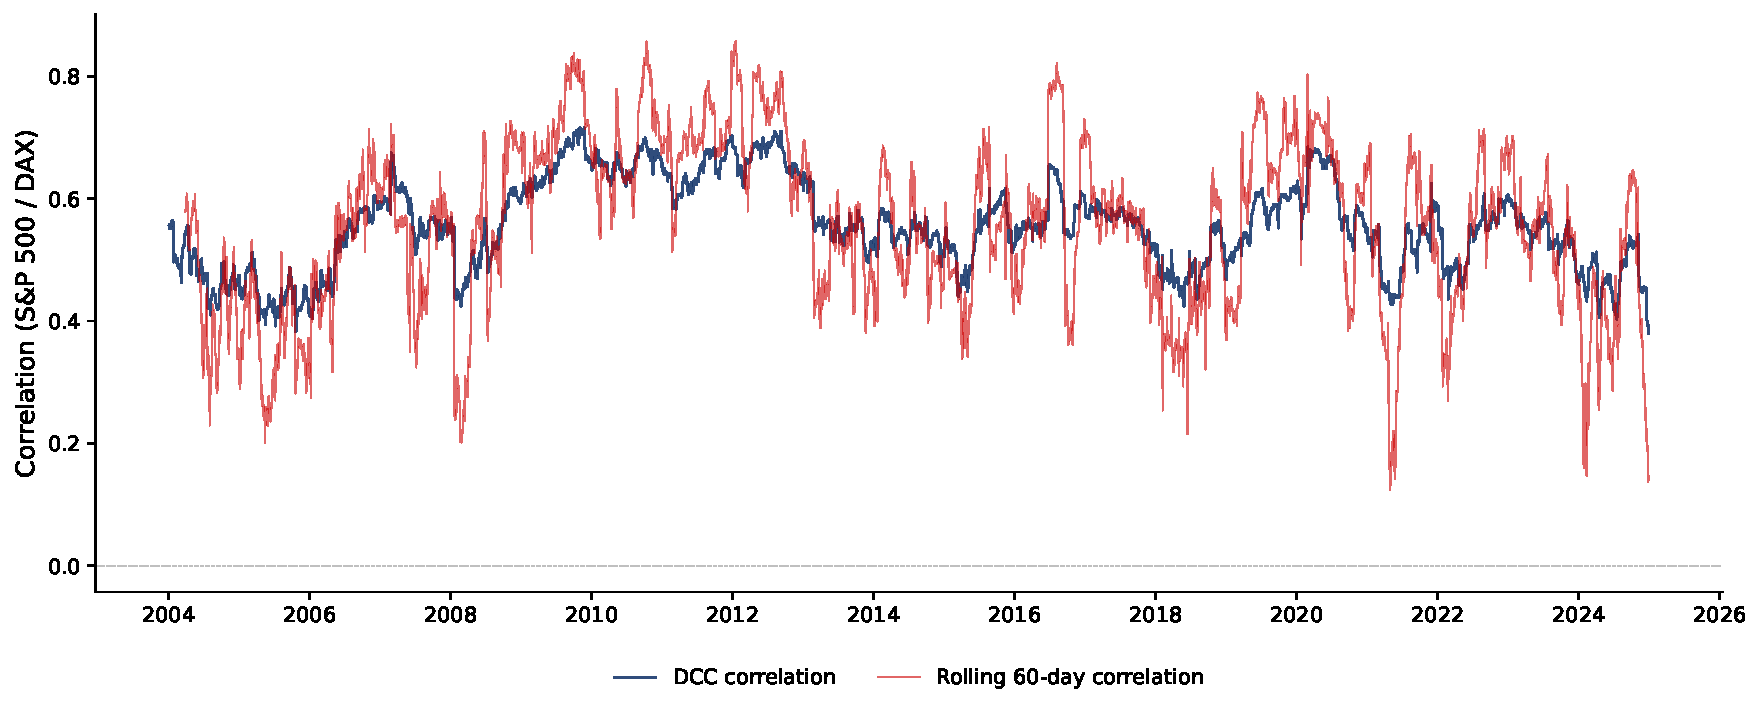
\includegraphics[width=0.95\textwidth, height=0.72\textheight, keepaspectratio]{../../charts/ch5b_dcc_vs_rolling.pdf}
        \end{center}
    \end{cminipage}
    \hfill\quantlet{TSA\_ch5b\_dcc\_estimation}{https://github.com/QuantLet/TSA/tree/main/TSA\_ch5b/TSA\_ch5b\_dcc\_estimation}
\end{frame}

\begin{frame}{Impactul știrilor asupra corelației DCC}
    \begin{cminipage}{0.95\textwidth}
    \vspace{-2mm}
        \begin{center}
            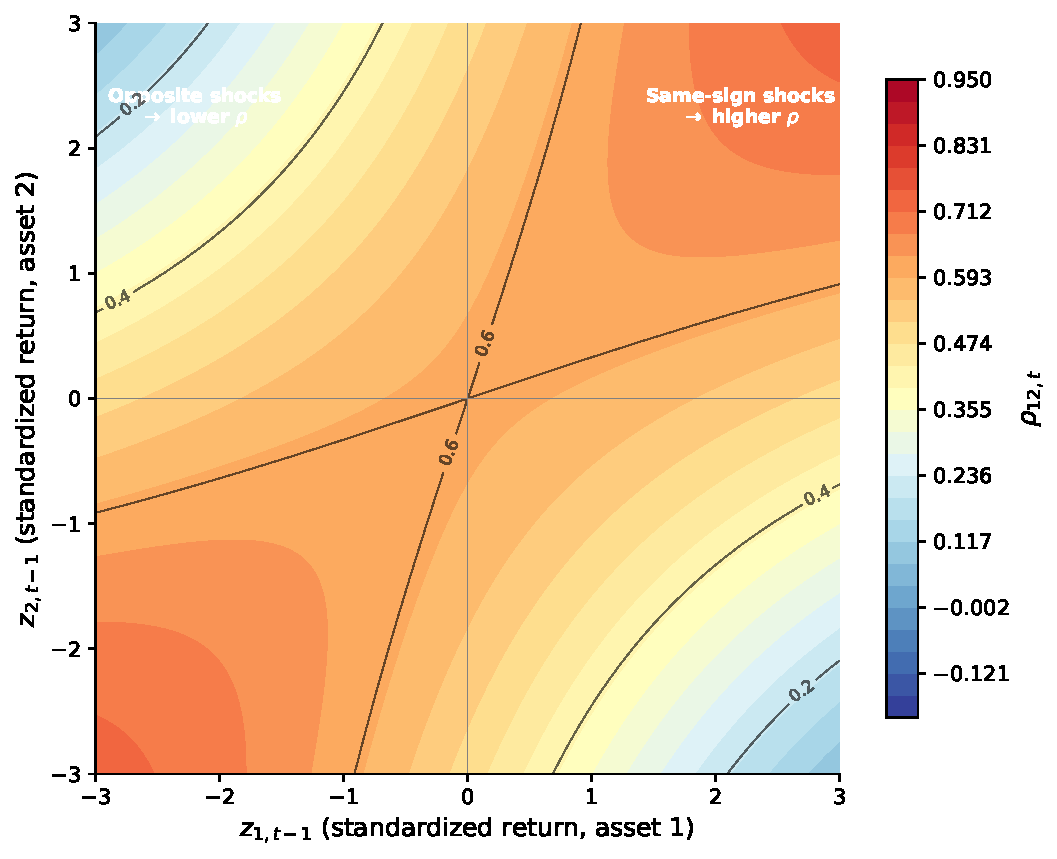
\includegraphics[width=0.85\textwidth, height=0.62\textheight, keepaspectratio]{../../charts/ch5b_news_impact_correlation.pdf}
        \end{center}
    \vspace{-2mm}
    {\footnotesize
    \begin{alertblock}{Interpretare}
        \begin{itemize}\setlength{\itemsep}{0pt}
            \item Când ambele active au șocuri de \textbf{același semn} (ambele pozitive sau ambele negative), corelația \textbf{crește}
            \item Șocurile de \textbf{semn opus} reduc corelația --- efect de decuplare
        \end{itemize}
    \end{alertblock}
    }
    \end{cminipage}
    \hfill\quantlet{TSA\_ch5b\_news\_impact\_corr}{https://github.com/QuantLet/TSA/tree/main/TSA\_ch5b/TSA\_ch5b\_news\_impact\_corr}
\end{frame}

\begin{frame}{Descompunerea covarianței: $\mathbf{H}_t = \mathbf{D}_t \mathbf{R}_t \mathbf{D}_t$}
    \begin{cminipage}{0.95\textwidth}
        \begin{center}
            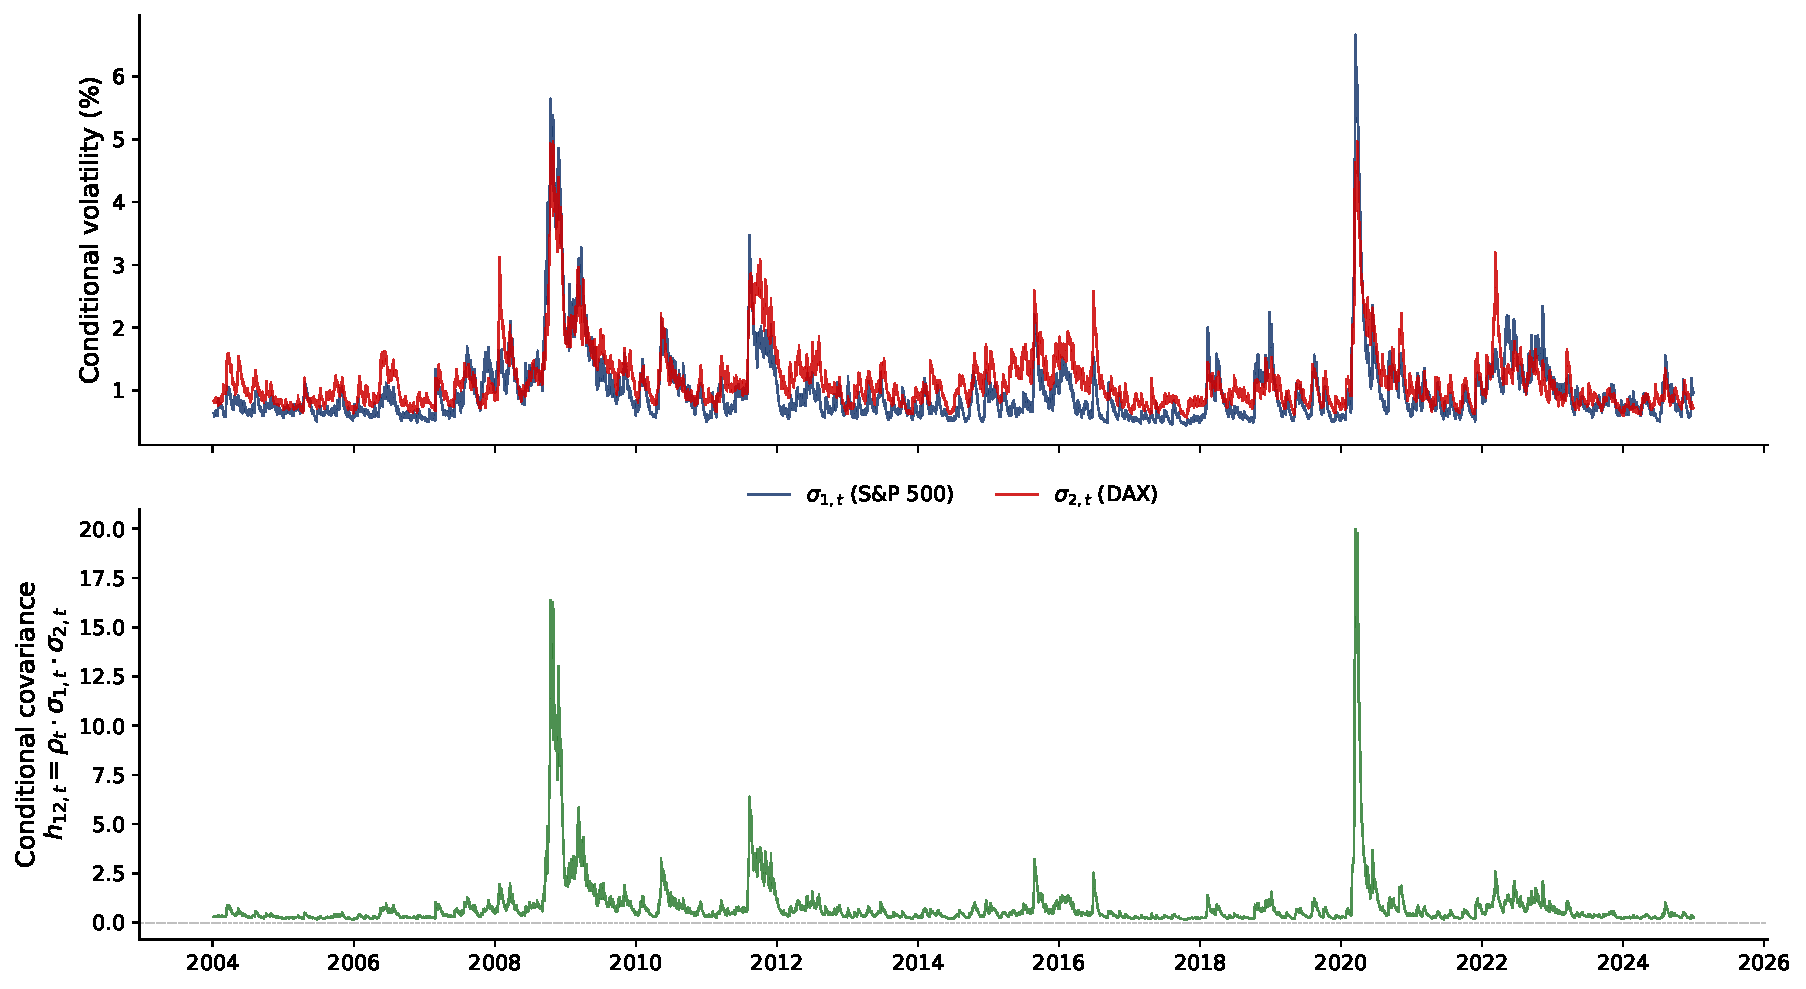
\includegraphics[width=0.95\textwidth, height=0.72\textheight, keepaspectratio]{../../charts/ch5b_covariance_decomp.pdf}
        \end{center}
    \end{cminipage}
    \hfill\quantlet{TSA\_ch5b\_cov\_decomp}{https://github.com/QuantLet/TSA/tree/main/TSA\_ch5b/TSA\_ch5b\_cov\_decomp}
\end{frame}

\begin{frame}{DCC vs CCC: când contează?}
    \begin{cminipage}{0.95\textwidth}
    {\footnotesize
    \begin{block}{Testarea corelației constante}
        \begin{itemize}\setlength{\itemsep}{0pt}
            \item \textbf{Testul Engle--Sheppard (2001)}: $H_0$: corelațiile sunt constante
                \begin{itemize}\setlength{\itemsep}{0pt}
                    \item Se regresează $\text{vech}(\mathbf{z}_t\mathbf{z}_t' - \hat{\mathbf{R}})$ pe valori decalate
                    \item $T \cdot R^2 \sim \chi^2$ sub $H_0$
                \end{itemize}
        \end{itemize}
    \end{block}
    \begin{block}{Evidențe empirice}
        \begin{itemize}\setlength{\itemsep}{0pt}
            \item CCC este aproape \textbf{întotdeauna respins} în datele financiare
            \item DCC oferă performanță out-of-sample mai bună pentru portofolii
            \item Îmbunătățirea este maximă în \textbf{perioadele de criză}
        \end{itemize}
    \end{block}
    \begin{alertblock}{Regulă practică}
        \begin{itemize}\setlength{\itemsep}{0pt}
            \item Utilizați CCC ca \textbf{benchmark} și DCC ca \textbf{model de bază}
            \item Dacă testul Engle--Sheppard respinge CCC, folosiți DCC
        \end{itemize}
    \end{alertblock}
    }
    \end{cminipage}
\end{frame}

\begin{frame}{Testul LM Tse (2000) pentru corelație constantă}
    \begin{cminipage}{0.95\textwidth}
    \vspace{-3mm}
    {\scriptsize
    \begin{block}{Ipoteze}
        \begin{itemize}\setlength{\itemsep}{0pt}
            \item $H_0$: $\rho_{ij,t} = \rho_{ij}$ $\forall t$ (corelațiile sunt \textbf{constante} --- modelul CCC este corect)
            \item $H_1$: $\rho_{ij,t}$ variază în timp (este necesar un model DCC)
        \end{itemize}
    \end{block}
    \vspace{-1mm}
    \begin{block}{Construcția testului}
        \begin{itemize}\setlength{\itemsep}{0pt}
            \item Se estimează modelul CCC și se obțin reziduurile standardizate $\hat{z}_{it} = \hat{\varepsilon}_{it}/\hat{\sigma}_{it}$
            \item Se calculează produsele pereche: $\hat{u}_{ij,t} = \hat{z}_{it}\hat{z}_{jt} - \hat{\rho}_{ij}$ pentru fiecare pereche $(i,j)$
            \item Se regresează $\hat{u}_{ij,t}$ pe $p$ valori decalate $\hat{u}_{ij,t-1}, \ldots, \hat{u}_{ij,t-p}$
            \item Statistica: $LM = T \sum_{i<j} R^2_{ij} \xrightarrow{d} \chi^2\big(\frac{N(N-1)}{2} \cdot p\big)$ sub $H_0$
        \end{itemize}
    \end{block}
    \vspace{-1mm}
    \begin{alertblock}{Diferența față de Engle--Sheppard (2001)}
        \begin{itemize}\setlength{\itemsep}{0pt}
            \item \textbf{Engle--Sheppard}: regresează vectorul $\text{vech}(\mathbf{z}_t\mathbf{z}_t' - \hat{\mathbf{R}})$ \textbf{simultan} pe valori decalate --- testează toate perechile într-o singură regresie
            \item \textbf{Tse}: testează fiecare pereche $(i,j)$ \textbf{separat}, apoi combină statisticile --- mai ușor de interpretat dar mai puțin puternic pentru dependențe complexe
        \end{itemize}
    \end{alertblock}
    }
    \end{cminipage}
\end{frame}

%=============================================================================
% DCC: PERSPECTIVĂ CHEIE + CAPCANE
%=============================================================================

\begin{frame}{DCC: perspectivă cheie și capcane frecvente}
    \begin{cminipage}{0.95\textwidth}
    \vspace{-3mm}
    {\scriptsize
    \begin{block}{\textcolor{MainBlue}{$\blacktriangleright$ Perspectivă cheie}: DCC captează dinamica corelațiilor cu doar 2 parametri}
        \begin{itemize}\setlength{\itemsep}{0pt}
            \item Puterea DCC: $a$ și $b$ sunt \textbf{comuni tuturor perechilor}
            \item Pentru 100 active, 4.950 de corelații evoluează cu aceeași viteză de reacție ($a$) și persistență ($b$)
            \item Aceasta este simultan cea mai mare forță și cea mai mare limitare
        \end{itemize}
    \end{block}
    \vspace{-2mm}
    \begin{alertblock}{\textcolor{Crimson}{$\blacktriangleright$ Capcane frecvente}}
        \begin{itemize}\setlength{\itemsep}{0pt}
            \item \textbf{Ignorarea Aielli (2013)}: DCC original cu $\bar{\mathbf{Q}} = E[\mathbf{z}_t\mathbf{z}_t']$ este inconsistent ($E[\mathbf{Q}_t] \neq \bar{\mathbf{Q}}$). cDCC corectează.
            \item \textbf{Presupunerea vitezei uniforme}: acțiuni-obligațiuni rapide, acțiuni-acțiuni lente --- un singur $(a,b)$ compromite
            \item \textbf{Forgetting the sandwich}: erorile standard naive din estimarea în 2 etape sunt \textbf{greșite} --- folosiți Bollerslev--Wooldridge
        \end{itemize}
    \end{alertblock}
    \vspace{-2mm}
    \begin{exampleblock}{\textcolor{Forest}{$\blacktriangleright$ Când NU se folosește DCC}}
        \begin{itemize}\setlength{\itemsep}{0pt}
            \item Nevoie de \textbf{direcția spillover}: DCC captează co-mișcarea dar nu care activ a cauzat șocul --- folosiți BEKK
            \item Corelații \textbf{genuine constante}: DCC adaugă zgomot; CCC este mai eficient
            \item Active cu \textbf{dinamici de corelație foarte diferite}: considerați block-DCC sau copula
        \end{itemize}
    \end{exampleblock}
    }
    \end{cminipage}
\end{frame}

\begin{frame}{Rezumatul secțiunii DCC}
    \begin{cminipage}{0.95\textwidth}
    {\footnotesize
    \begin{block}{3 lucruri de reținut}
        \begin{enumerate}\setlength{\itemsep}{2pt}
            \item DCC = CCC cu $\mathbf{R}_t$ dinamic: doar \textbf{2 parametri suplimentari} ($a, b$) pentru toate cele $N(N-1)/2$ corelații
            \item Ecuația $\mathbf{Q}_t$ este un GARCH(1,1) pentru corelații: $a$ = reactivitate la șocuri, $b$ = persistență
            \item Estimarea în două etape este consistentă dar necesită \textbf{erori standard sandwich}
        \end{enumerate}
    \end{block}
    \begin{alertblock}{Poziționarea modelului}
        \begin{itemize}\setlength{\itemsep}{0pt}
            \item \textbf{Utilizare}: \textbf{calul de bătaie} al industriei --- cel mai bun echilibru între flexibilitate și scalabilitate
            \item \textbf{vs.\ CCC}: captează vârfurile de corelație din crize \quad \textbf{vs.\ BEKK}: fără direcție de spillover, dar scalează la $N > 100$
        \end{itemize}
    \end{alertblock}
    \vspace{1mm}
    \textit{\textbf{Concluzie cheie:} DCC este standardul industrial --- 2 parametri captează toate cele $N(N-1)/2$ corelații dinamice.}
    }
    \end{cminipage}
\end{frame}

%=============================================================================
% SECȚIUNEA 7: ALTE MODELE GARCH MULTIVARIATE
%=============================================================================
\section{Alte modele GARCH multivariate}

\begin{frame}{DCC Asimetric (aDCC) -- Cappiello, Engle \& Sheppard (2006)}
    \begin{cminipage}{0.95\textwidth}
    {\footnotesize
    \begin{block}{Motivație: levier în corelații}
        \begin{itemize}\setlength{\itemsep}{0pt}
            \item Corelațiile răspund asimetric la șocuri negative vs.\ pozitive
            \item aDCC extinde DCC cu un termen asimetric:
            \[
                \mathbf{Q}_t = (\bar{\mathbf{Q}} - a\bar{\mathbf{Q}} - b\bar{\mathbf{Q}} - g\bar{\mathbf{N}}) + a\,\mathbf{z}_{t-1}\mathbf{z}_{t-1}' + b\,\mathbf{Q}_{t-1} + g\,\underbrace{\mathbf{n}_{t-1}\mathbf{n}_{t-1}'}_{\text{termen asimetric}}
            \]
            \item $\mathbf{n}_t = \mathbf{z}_t \odot \mathbf{1}(\mathbf{z}_t < 0)$ și $\bar{\mathbf{N}} = T^{-1}\sum_t \mathbf{n}_t\mathbf{n}_t'$
        \end{itemize}
        \textit{Intuiție: pierderile comune (termenul $g$) pot crește corelațiile mai mult decât câștigurile comune --- ``amplificatorul de vești proaste.''}
    \end{block}
    \begin{block}{Proprietăți}
        \begin{itemize}\setlength{\itemsep}{0pt}
            \item Adaugă doar \textbf{un parametru} ($g$) la modelul DCC
            \item Captează empiric: corelațiile cresc mai mult după \textbf{șocuri negative comune}
            \item Include DCC ($g=0$) și CCC ($a=b=g=0$) ca și cazuri particulare
        \end{itemize}
    \end{block}
    }
    \end{cminipage}
\end{frame}

\begin{frame}{GO-GARCH (van der Weide, 2002)}
    \begin{cminipage}{0.95\textwidth}
    \vspace{-1mm}
    {\footnotesize
    \begin{block}{Ideea: GARCH ortogonal generalizat}
        \begin{itemize}\setlength{\itemsep}{0pt}
            \item Se transformă vectorul $N$-dimensional în $N$ \textbf{factori necorelați}:
            \[
                \boldsymbol{\varepsilon}_t = \mathbf{Z}\mathbf{f}_t, \qquad \mathbf{f}_t = (f_{1t}, \ldots, f_{Nt})'
            \]
            \item $\mathbf{Z}$: matrice de mixare; fiecare factor $f_{it}$ are dinamică GARCH individuală:
            \[
                \sigma_{f_i,t}^2 = \omega_i + \alpha_i f_{i,t-1}^2 + \beta_i \sigma_{f_i,t-1}^2
            \]
        \end{itemize}
    \end{block}
    \begin{block}{Reconstrucție}
        \[
            \mathbf{H}_t = \mathbf{Z}\,\text{diag}(\sigma_{f_1,t}^2, \ldots, \sigma_{f_N,t}^2)\,\mathbf{Z}'
        \]
        \textit{Intuiție: se modelează volatilitatea în ``spațiul factorilor'' (simplu), apoi se rotește înapoi în ``spațiul activelor'' (complex).}
        \begin{itemize}\setlength{\itemsep}{0pt}
            \item Pozitiv definită \textbf{prin construcție}
            \item Parametri: $N(N-1)/2 + 3N$ --- scalează bine cu $N$
            \item Legat de Analiza Componentelor Independente (ICA)
        \end{itemize}
    \end{block}
    }
    \end{cminipage}
\end{frame}

\begin{frame}{Modele GARCH factoriale}
    \begin{cminipage}{0.95\textwidth}
    \vspace{-3mm}
    {\scriptsize
    \begin{block}{Ideea: reducerea dimensionalității cu factori ($K \ll N$)}
        \begin{itemize}\setlength{\itemsep}{0pt}
            \item Model factorial:
            $\boldsymbol{\varepsilon}_t = \mathbf{\Lambda}\mathbf{f}_t + \mathbf{u}_t$
            \item $\mathbf{\Lambda}$: $N \times K$ (încărcături); $\mathbf{f}_t$: $K \times 1$ (factori comuni); $\mathbf{u}_t$: idiosincratic
            \item Covarianța condițională:
            $\mathbf{H}_t = \underbrace{\mathbf{\Lambda}\mathbf{H}_t^f\mathbf{\Lambda}'}_{\text{risc sistematic}} + \underbrace{\boldsymbol{\Sigma}_t^u}_{\text{risc idiosincratic}}$
        \end{itemize}
        \textit{Intuiție: se modelează câțiva factori comuni, restul se tratează ca zgomot.}
    \end{block}
    \vspace{-2mm}
    \begin{block}{Variante}
        \begin{itemize}\setlength{\itemsep}{0pt}
            \item \textbf{O-GARCH} (Alexander, 2001): factori din PCA (\textit{Principal Component Analysis}), GARCH pe componente principale
            \item \textbf{Factor GARCH} (Engle, Ng \& Rothschild, 1990): structură parametrică
            \item \textbf{DCC-MIDAS} (Colacito, Engle \& Ghysels, 2011): frecvență mixtă
        \end{itemize}
    \end{block}
    \begin{alertblock}{Când se utilizează}
        \begin{itemize}\setlength{\itemsep}{0pt}
            \item Abordarea \textbf{de referință} pentru $N$ mare (50--500 active): \textit{parsimony} + interpretabilitate economică.
        \end{itemize}
    \end{alertblock}
    }
    \end{cminipage}
\end{frame}

\begin{frame}{Modelul DCC Tse--Tsui (2002)}
    \begin{cminipage}{0.95\textwidth}
    {\footnotesize
    \begin{block}{O alternativă la DCC-ul lui Engle}
        \begin{itemize}\setlength{\itemsep}{0pt}
            \item Tse \& Tsui (2002) propun o dinamică diferită pentru $\mathbf{R}_t$:
            \[
                \mathbf{R}_t = (1 - \theta_1 - \theta_2)\underbrace{\mathbf{R}}_{\text{termen lung}} + \theta_1 \underbrace{\boldsymbol{\Psi}_{t-1}}_{\text{fereastră locală}} + \theta_2 \underbrace{\mathbf{R}_{t-1}}_{\text{persistență}}
            \]
            \item \textit{Intuiție: se combină corelația pe termen lung, fereastra recentă și corelația de ieri --- rezultatul este automat o matrice de corelație validă.}
            \item $\boldsymbol{\Psi}_{t-1}$ = corelația reziduurilor standardizate din ultimele $M$ observații
        \end{itemize}
    \end{block}
    \begin{block}{Comparație cu DCC Engle}
        \begin{itemize}\setlength{\itemsep}{0pt}
            \item \textbf{Avantaj}: $\mathbf{R}_t$ este matrice de corelație \textbf{prin construcție} (fără rescalare)
            \item \textbf{Dezavantaj}: necesită alegerea ferestrei $M$; mai puțin folosit în practică
            \item Ambele modele produc rezultate similare empiric
        \end{itemize}
    \end{block}
    }
    \end{cminipage}
\end{frame}

\begin{frame}{Copula-GARCH: o abordare flexibilă}
    \begin{cminipage}{0.95\textwidth}
    {\footnotesize
    \begin{block}{Ideea: separarea marginilelor de structura de dependență}
        \begin{itemize}\setlength{\itemsep}{0pt}
            \item \textbf{Teorema lui Sklar}: $F(x_1, \ldots, x_N) = C\big(F_1(x_1), \ldots, F_N(x_N)\big)$
            \item \textit{Intuiție: se modelează profilul de risc al fiecărui activ separat, apoi se ``lipesc'' împreună cu o copulă.}
            \item $F_i$ = distribuțiile marginale (fiecare modelată cu GARCH + distribuție flexibilă)
            \item $C$ = copula care captează structura de dependență
        \end{itemize}
    \end{block}
    \begin{block}{Avantaje față de DCC}
        \begin{itemize}\setlength{\itemsep}{0pt}
            \item Permite \textbf{dependență asimetrică în cozi} (\textit{tail dependence})
            \item Marginilele pot avea distribuții \textbf{diferite} (Student-$t$, skewed-$t$, GED --- \textit{Generalized Error Distribution})
            \item Copula $t$-Student: $\rho_t$ din DCC + dependență de coadă parametrizată de $\nu$
        \end{itemize}
    \end{block}
    \begin{alertblock}{Implementare}
        \begin{itemize}\setlength{\itemsep}{0pt}
            \item Pachetul R \texttt{copula} + \texttt{rugarch}; Python: \texttt{copulae}
        \end{itemize}
    \end{alertblock}
    }
    \end{cminipage}
\end{frame}

\begin{frame}{EWMA și RiskMetrics}
    \begin{cminipage}{0.95\textwidth}
    {\footnotesize
    \begin{block}{EWMA (\textit{Exponentially Weighted Moving Average})}
        \begin{itemize}\setlength{\itemsep}{0pt}
            \item Cel mai simplu model multivariat de volatilitate --- fără estimare:
        \end{itemize}
        \[
            \mathbf{H}_t = (1-\lambda)\boldsymbol{\varepsilon}_{t-1}\boldsymbol{\varepsilon}_{t-1}' + \lambda\mathbf{H}_{t-1}, \qquad \lambda = 0.94 \text{ (date zilnice)}
        \]
        \textit{Intuiție: o medie ponderată între prognoza de ieri și șocurile realizate ieri --- fără estimare necesară.}
    \end{block}
    \begin{block}{Legătura cu MGARCH}
        \begin{itemize}\setlength{\itemsep}{0pt}
            \item EWMA $\equiv$ BEKK Scalar cu $\omega = 0$, $a^2 = 1-\lambda$, $b^2 = \lambda$
            \item Echivalent cu IGARCH ($\alpha + \beta = 1$) fără interceptare
            \item RiskMetrics (J.P.\ Morgan, 1996): \textbf{standard industrial} bazat pe EWMA
        \end{itemize}
    \end{block}
    \begin{alertblock}{Limitări}
        \begin{itemize}\setlength{\itemsep}{0pt}
            \item Fără estimare $\Rightarrow$ nu se poate adapta la condiții diferite de piață
            \item $\lambda = 0.94$ poate să nu fie optim pentru toate clasele de active
            \item Fără efecte asimetrice, fără revenire la medie a varianței
        \end{itemize}
    \end{alertblock}
    }
    \end{cminipage}
\end{frame}

\begin{frame}{Taxonomia modelelor: rezumat}
    \begin{cminipage}{0.95\textwidth}
    {\scriptsize
    \begin{center}
    \begin{tabular}{lcccc}
        \hline
        \textbf{Model} & \textbf{P.D.} & \textbf{Spillovers} & \textbf{$\rho$ dinamic} & \textbf{Max $N$} \\
        \hline
        VEC & Nu$^*$ & Da & Da & $\sim 3$ \\
        VEC Diagonal & Da$^*$ & Nu & Da & $\sim 10$ \\
        BEKK (complet) & Da & Da & Da & $\sim 5$ \\
        BEKK Diagonal & Da & Nu & Da & $\sim 20$ \\
        BEKK Scalar / EWMA & Da & Nu & Da & $\sim 100$ \\
        CCC & Da & Nu & Nu & $\sim 100$ \\
        DCC & Da & Nu & Da & $\sim 500$ \\
        aDCC & Da & Nu & Da & $\sim 500$ \\
        GO-GARCH & Da & Nu & Da & $\sim 50$ \\
        Factor GARCH & Da & Nu & Da & $\sim 500$ \\
        \hline
    \end{tabular}
    \end{center}
    \vspace{0.1cm}
    $^*$ Necesită restricții suplimentare pe parametri.
    }
    \begin{alertblock}{}
        {\footnotesize
        \begin{itemize}\setlength{\itemsep}{0pt}
            \item Alegerea modelului depinde de: (1) numărul de active, (2) nevoia de spillovers, (3) corelații dinamice, (4) bugetul computațional
        \end{itemize}
        }
    \end{alertblock}
    \end{cminipage}
\end{frame}

\begin{frame}{Ierarhia modelelor GARCH multivariate}
    \begin{cminipage}{0.95\textwidth}
    {\footnotesize
    \begin{block}{Relații de includere (\textit{nesting})}
        \begin{itemize}\setlength{\itemsep}{0pt}
            \item EWMA $\subset$ BEKK Scalar $\subset$ BEKK Diagonal $\subset$ BEKK Complet $\subset$ VEC Complet
            \item CCC $\subset$ DCC $\subset$ aDCC
            \item DCC și BEKK Diagonal: \textbf{nu} sunt incluse unul în celălalt
        \end{itemize}
    \end{block}
    \begin{block}{Alegerea în funcție de obiectiv}
        \vspace{0.1cm}
        \begin{center}
        {\scriptsize
        \begin{tabular}{lll}
            \hline
            \textbf{Obiectiv} & \textbf{Model recomandat} & \textbf{De ce} \\
            \hline
            VaR de portofoliu & DCC / aDCC & Corelații dinamice, scalabil \\
            Hedging optim & DCC / BEKK Diag & Cov.\ variabilă în timp \\
            Propagare șocuri & BEKK Complet & Captează spillovers \\
            $N > 100$ active & Factor GARCH / DCC & Parcimonie, fezabilitate \\
            Asimetrie corelații & aDCC & Termenul $g$ pentru levier \\
            Dependență de coadă & Copula-GARCH & Flexibilitate distribuțională \\
            \hline
        \end{tabular}
        }
        \end{center}
    \end{block}
    }
    \end{cminipage}
\end{frame}

%=============================================================================
% SECȚIUNEA 8: LIMITĂRI ALE MODELELOR MGARCH
%=============================================================================
\section{Limitări ale modelelor MGARCH}

\begin{frame}{Când eșuează modelele MGARCH}
    \begin{cminipage}{0.95\textwidth}
    \vspace{-3mm}
    {\scriptsize
    \begin{block}{Specificare greșită a modelului}
        \begin{itemize}\setlength{\itemsep}{0pt}
            \item Toate modelele MGARCH presupun o \textbf{structură parametrică} pentru $\mathbf{H}_t$ --- procesul real poate să nu aparțină acestei clase
            \item DCC presupune \textbf{o singură dinamică a corelației pentru toate perechile}: $a$, $b$ scalari, deși perechile acțiuni-obligațiuni și acțiuni-acțiuni se comportă diferit
            \item BEKK impune dinamici \textbf{pătratice} --- nu poate capta schimbări de regim sau \textit{structural breaks}
            \item QML Gaussian: \textbf{consistent dar ineficient} sub cozi groase --- pierderile de eficiență cresc cu $N$
        \end{itemize}
    \end{block}
    \vspace{-2mm}
    \begin{block}{\textit{Tail risk failures}}
        \begin{itemize}\setlength{\itemsep}{0pt}
            \item MGARCH cu inovații normale \textbf{subestimează riscul comun din cozi}: $\Pr(\text{toate activele cad})$ prea mic
            \item Copula Student-$t$ ajută, dar presupune dependență de coadă \textbf{simetrică} --- activele cad împreună dar nu cresc împreună
            \item Violările VaR în crize sunt \textbf{grupate} --- chiar DCC cu acoperire corectă are violări concentrate
        \end{itemize}
    \end{block}
    \vspace{-2mm}
    \begin{alertblock}{Concluzie}
        \begin{itemize}\setlength{\itemsep}{0pt}
            \item Modelele MGARCH sunt \textbf{aproximări locale} --- funcționează bine în regimuri stabile dar subperformează în tranziții de regim
        \end{itemize}
    \end{alertblock}
    }
    \end{cminipage}
\end{frame}

\begin{frame}{Instabilitate în criză și paradoxul DCC}
    \begin{cminipage}{0.95\textwidth}
    \vspace{-3mm}
    {\scriptsize
    \begin{block}{Paradoxul DCC}
        \begin{itemize}\setlength{\itemsep}{0pt}
            \item DCC este \textbf{cel mai necesar} în crize --- dar crizele sunt exact momentul când este \textbf{cel mai puțin fiabil}
            \item Estimările parametrilor din perioade de calm pot \textbf{să nu se aplice} dinamicilor de criză
            \item Aielli (2013): estimatorul DCC standard are \textbf{bias} în procedura în două etape --- cDCC corectează
        \end{itemize}
    \end{block}
    \vspace{-2mm}
    \begin{block}{\textit{Structural breaks} în corelații}
        \begin{itemize}\setlength{\itemsep}{0pt}
            \item \textbf{Euro (1999)}: corelațiile acțiunilor europene au crescut permanent
            \item \textbf{GFC (2008)}: corelațiile \textit{cross-asset} au sărit și nu au revenit complet ani de zile
            \item \textbf{COVID (2020)}: salt de corelație fără precedent urmat de \textit{decorrelation} rapidă
            \item Revenirea la medie DCC ($a + b < 1$) forțează corelațiile la $\bar{Q}$ --- poate fi \textbf{greșit} după \textit{structural breaks}
        \end{itemize}
    \end{block}
    \vspace{-2mm}
    \begin{alertblock}{Remedii}
        \begin{itemize}\setlength{\itemsep}{0pt}
            \item \textbf{DCC-MIDAS} (Colacito, Engle \& Ghysels, 2011): separă corelația pe termen scurt și lung
            \item \textbf{\textit{Markov-Switching} DCC}: schimbări discrete de regim în dinamica corelațiilor
            \item \textbf{Ferestre mobile}: re-estimare la fiecare 1--2 ani pentru schimbări structurale
        \end{itemize}
    \end{alertblock}
    }
    \end{cminipage}
\end{frame}

\begin{frame}{\textit{Overfitting} vs.\ \textit{parsimony}: compromisul \textit{bias-variance}}
    \begin{cminipage}{0.95\textwidth}
    \vspace{-2mm}
    {\scriptsize
    \begin{block}{Capcana \textit{overfitting}-ului}
        \begin{itemize}\setlength{\itemsep}{0pt}
            \item BEKK complet pentru $N = 5$: \textbf{55 parametri} --- se potrivește perfect \textit{in-sample}, slab \textit{out-of-sample}
            \item aDCC ($+1$ parametru) ajută pentru acțiuni dar poate face \textit{overfit} pe perechi obligațiuni-mărfuri
            \item Gradele de libertate Student-$t$ ($\nu$) pot \textbf{compensa} specificarea greșită, mascând problema reală
        \end{itemize}
    \end{block}
    \vspace{-1mm}
    \begin{block}{Evidențe empirice (Caporin \& McAleer, 2012; Laurent et al., 2012)}
        \begin{itemize}\setlength{\itemsep}{0pt}
            \item \textbf{Scalar BEKK $\approx$ DCC} în previziunea \textit{out-of-sample} pentru majoritatea portofoliilor
            \item Adăugarea complexității dincolo de DCC(1,1) rareori îmbunătățește VaR-ul sau eficacitatea \textit{hedging}-ului
            \item \textbf{EWMA simplu ($\lambda = 0.94$)} rămâne un \textit{benchmark} competitiv --- greu de bătut consistent
            \item Criteriile informaționale (AIC/BIC) favorizează DCC față de BEKK pentru $N > 3$
        \end{itemize}
    \end{block}
    \begin{alertblock}{Regulă practică}
        \begin{itemize}\setlength{\itemsep}{0pt}
            \item Începeți simplu (EWMA sau CCC), adăugați complexitate \textbf{doar dacă testele \textit{out-of-sample} o justifică}
            \item Utilizați \textbf{\textit{Model Confidence Sets}} (Hansen, Lunde \& Nason, 2011) în loc de selecție pe un singur model
        \end{itemize}
    \end{alertblock}
    }
    \end{cminipage}
\end{frame}

\begin{frame}{Comparație empirică între modele: ce arată literatura}
    \begin{cminipage}{0.95\textwidth}
    \vspace{-3mm}
    {\scriptsize
    \begin{block}{Performanța \textit{out-of-sample} (bazat pe Laurent et al., 2012; Caporin \& McAleer, 2014)}
        \vspace{-1mm}
        \begin{center}
        \begin{tabular}{lccccc}
            \hline
            \textbf{Model} & \textbf{VaR portf.} & \textbf{\textit{Hedge}} & \textbf{GMVP} & \textbf{Viteză} & \textbf{Max $N$} \\
            \hline
            EWMA ($\lambda\!=\!0.94$) & Bun & Mediu & Mediu & $\star\star\star\star\star$ & 1000+ \\
            CCC-GARCH & Mediu & Mediu & Slab & $\star\star\star\star$ & 500 \\
            DCC-GARCH & \textbf{Bun} & \textbf{Bun} & Bun & $\star\star\star\star$ & 500 \\
            aDCC-GARCH & \textbf{Bun} & \textbf{Bun} & \textbf{Bun} & $\star\star\star$ & 300 \\
            Diagonal BEKK & Bun & Bun & Bun & $\star\star\star$ & 20 \\
            BEKK complet & Mediu$^*$ & Bun & Mediu$^*$ & $\star$ & 5 \\
            GO-GARCH & Bun & Mediu & Bun & $\star\star$ & 50 \\
            Copula-DCC & \textbf{Cel mai bun} & Bun & Bun & $\star\star$ & 100 \\
            \hline
        \end{tabular}
        \end{center}
        \vspace{-2mm}
        $^*$BEKK complet face \textit{overfit in-sample}, se degradează \textit{out-of-sample} pentru $N > 3$. GMVP = \textit{Global Minimum Variance Portfolio}.
    \end{block}
    \vspace{-2mm}
    \begin{alertblock}{Concluzii cheie}
        \begin{itemize}\setlength{\itemsep}{0pt}
            \item DCC este \textbf{cea mai bună alegere ajustată la risc} pentru majoritatea aplicațiilor
            \item Copula-DCC domină pentru \textbf{\textit{tail risk}} (ES, VaR extrem) dar la cost computațional mai mare
            \item Complexitatea dincolo de aDCC produce \textbf{randamente descrescătoare} pentru majoritatea portofoliilor
        \end{itemize}
    \end{alertblock}
    }
    \end{cminipage}
\end{frame}

%=============================================================================
% SECȚIUNEA 9: ESTIMARE ȘI DIAGNOSTICE
%=============================================================================
\section{Estimare și diagnostice}

\begin{frame}{Metode de estimare}
    \begin{cminipage}{0.95\textwidth}
    {\footnotesize
    \begin{block}{Estimare prin verosimilitate maximă (MLE)}
        \begin{itemize}\setlength{\itemsep}{0pt}
            \item \textbf{MLE complet}: estimare simultană a tuturor parametrilor --- optimal dar costisitor
            \item \textbf{MLE în două etape (compozit)}: univariat mai întâi, apoi corelație
                \begin{itemize}\setlength{\itemsep}{0pt}
                    \item Utilizat de CCC, DCC, aDCC
                    \item Consistent dar mai puțin eficient decât MLE complet
                \end{itemize}
        \end{itemize}
    \end{block}
    \begin{block}{Quasi-verosimilitate maximă (QML)}
        \begin{itemize}\setlength{\itemsep}{0pt}
            \item Se utilizează verosimilitatea Gaussiană chiar dacă distribuția reală este non-Gaussiană
            \item Estimatorul QML este \textbf{consistent} sub condiții de regularitate ușoare
            \item \textbf{Erori standard robuste (sandwich)}: $\hat{V} = \hat{J}^{-1}\hat{I}\hat{J}^{-1}$
        \end{itemize}
    \end{block}
    \begin{block}{Alternativă: Student-$t$ multivariat}
        \begin{itemize}\setlength{\itemsep}{0pt}
            \item Captează mai bine cozile groase: $\mathbf{z}_t \sim t_\nu(\mathbf{0}, \mathbf{I}_N)$
            \item Adaugă un parametru ($\nu$) pentru grade de libertate
        \end{itemize}
    \end{block}
    }
    \end{cminipage}
\end{frame}

\begin{frame}{Estimatorul sandwich (\textit{Sandwich Estimator})}
    \begin{cminipage}{0.95\textwidth}
    \vspace{-3mm}
    {\scriptsize
    \begin{block}{De ce este necesar?}
        \begin{itemize}\setlength{\itemsep}{0pt}
            \item QML presupune distribuție Gaussiană, dar datele financiare au \textbf{cozi groase} și \textbf{asimetrie}
            \item Parametrii sunt \textbf{consistenți}, dar erorile standard clasice sunt \textbf{incorecte}
            \item Soluția: estimatorul \textbf{sandwich} Bollerslev--Wooldridge (1992) corectează erorile standard
        \end{itemize}
    \end{block}
    \vspace{-3mm}
    \begin{block}{Structura ``sandwich'' --- de unde vine numele}
        \begin{itemize}\setlength{\itemsep}{0pt}
            \item Matricea de varianță-covarianță a estimatorului: $\hat{V}(\hat{\boldsymbol{\theta}}) = \underbrace{\hat{\mathbf{J}}^{-1}}_{\text{``pâine''}} \underbrace{\hat{\mathbf{I}}}_{\text{``umplutură''}} \underbrace{\hat{\mathbf{J}}^{-1}}_{\text{``pâine''}}$
            \item $\hat{\mathbf{J}} = -\frac{1}{T}\sum_t \frac{\partial^2 \ell_t}{\partial \boldsymbol{\theta}\partial \boldsymbol{\theta}'}$ \quad (Hessianul --- presupune modelul corect)
            \item $\hat{\mathbf{I}} = \frac{1}{T}\sum_t \frac{\partial \ell_t}{\partial \boldsymbol{\theta}} \frac{\partial \ell_t}{\partial \boldsymbol{\theta}'}$ \quad (produsul exterior al gradienților --- \textit{empiric}, fără presupuneri)
            \item \textit{Intuiție: $\hat{\mathbf{J}}$ are încredere în model; $\hat{\mathbf{I}}$ are încredere în date. Dacă modelul e corect, $\mathbf{I} = \mathbf{J}$ și $\hat{V} = \mathbf{J}^{-1}$.}
        \end{itemize}
    \end{block}
    \vspace{-2mm}
    \begin{alertblock}{Când se folosește}
        \begin{itemize}\setlength{\itemsep}{0pt}
            \item \textbf{Întotdeauna} la estimare QML (GARCH cu verosimilitate Gaussiană pe date non-Gaussiene)
            \item La estimarea DCC în două etape: erorile standard din etapa 2 trebuie corectate pentru incertitudinea din etapa 1
        \end{itemize}
    \end{alertblock}
    }
    \end{cminipage}
\end{frame}

\begin{frame}{Verificări diagnostice}
    \begin{cminipage}{0.95\textwidth}
    {\footnotesize
    \begin{block}{Diagnostice pe reziduuri}
        \begin{itemize}\setlength{\itemsep}{0pt}
            \item Se calculează reziduurile standardizate $\hat{\mathbf{z}}_t = \hat{\mathbf{D}}_t^{-1}\hat{\boldsymbol{\varepsilon}}_t$ și se verifică:
                \begin{enumerate}\setlength{\itemsep}{0pt}
                    \item \textbf{Absența corelației seriale} în $\hat{z}_{it}$ și $\hat{z}_{it}^2$ (Ljung--Box)
                    \item \textbf{Absența corelației încrucișate} în $\hat{z}_{it}\hat{z}_{jt}$ (Hosking, 1980)
                    \item \textbf{Normalitatea} lui $\hat{\mathbf{z}}_t$ (dacă s-a presupus verosimilitate Gaussiană)
                \end{enumerate}
        \end{itemize}
    \end{block}
    \begin{block}{Compararea modelelor}
        \begin{itemize}\setlength{\itemsep}{0pt}
            \item \textbf{Criterii informaționale}: AIC, BIC (\textit{Akaike/Bayesian Information Criterion}) (penalizează supra-parametrizarea)
            \item \textbf{Teste ale raportului de verosimilitate}: modele imbricate (CCC vs DCC)
            \item \textbf{Evaluare out-of-sample}: performanța portofoliului, backtesting VaR
            \item \textbf{Regresie Mincer--Zarnowitz}: prognoza $\hat{h}_{ij,t}$ vs covarianța realizată
        \end{itemize}
    \end{block}
    }
    \end{cminipage}
\end{frame}

\begin{frame}{Estimare practică: sfaturi și capcane}
    \begin{cminipage}{0.95\textwidth}
    {\footnotesize
    \begin{block}{Sfaturi practice (\textit{tips \& tricks})}
        \begin{itemize}\setlength{\itemsep}{0pt}
            \item \textbf{Valori inițiale}: porniți de la estimări OLS (\textit{Ordinary Least Squares}) sau de la EWMA ($\lambda = 0.94$)
            \item \textbf{Randamente}: folosiți log-randamente $\times 100$ (în procente) --- stabilizează optimizarea
            \item \textbf{Date lipsă}: aliniați seriile pe datele comune; nu interpolați
            \item \textbf{Convergență}: rulați optimizarea din mai multe puncte de start
        \end{itemize}
    \end{block}
    \begin{alertblock}{Capcane frecvente}
        \begin{itemize}\setlength{\itemsep}{0pt}
            \item \textbf{Tranzacționare nesincronizată} (\textit{nonsynchronous trading}): DAX închide la 17:30 CET, NYSE la 16:00 EST --- corelațiile intra-zilnice sunt subestimate
                \begin{itemize}\setlength{\itemsep}{0pt}
                    \item Soluție: corecția Scholes--Williams (1977) sau utilizarea randamentelor deschidere-la-deschidere
                \end{itemize}
            \item \textbf{Rupturi structurale}: crize modifică permanent regimul de corelații --- DCC presupune un singur regim
            \item \textbf{Supraevaluarea Student-$t$}: gradele de libertate $\nu$ pot compensa alte probleme de specificare
        \end{itemize}
    \end{alertblock}
    }
    \end{cminipage}
\end{frame}

\begin{frame}{Selecția modelului: ghid practic}
    \begin{cminipage}{0.95\textwidth}
    {\footnotesize
    \begin{block}{Diagramă de decizie}
        \begin{enumerate}\setlength{\itemsep}{2pt}
            \item \textbf{Câte active?}
                \begin{itemize}\setlength{\itemsep}{0pt}
                    \item $N \leq 5$: BEKK, DCC sau aDCC
                    \item $5 < N \leq 50$: DCC, aDCC, GO-GARCH
                    \item $N > 50$: Factor GARCH, DCC-MIDAS, EWMA
                \end{itemize}
            \item \textbf{Aveți nevoie de propagare de volatilitate (spillovers)?}
                \begin{itemize}\setlength{\itemsep}{0pt}
                    \item Da: BEKK complet ($N$ mic) sau modele factoriale
                    \item Nu: familia DCC
                \end{itemize}
            \item \textbf{Există asimetrie în corelații?}
                \begin{itemize}\setlength{\itemsep}{0pt}
                    \item Testați $\Rightarrow$ dacă da, utilizați aDCC
                \end{itemize}
            \item \textbf{Validare}: diagnostice pe reziduuri, performanța out-of-sample
        \end{enumerate}
    \end{block}
    }
    \end{cminipage}
\end{frame}

%=============================================================================
% SECȚIUNEA 9: STUDII DE CAZ ȘI APLICAȚII
%=============================================================================
\section{Studii de caz}

%--- Studiu de caz 1: Propagarea volatilității ---
\begin{frame}{Studiu de caz 1: propagarea volatilității între piețe}
    \vspace{-2mm}
    {\scriptsize\textit{Obiectiv didactic: cum elementele off-diagonale din BEKK indică direcția transmisiei șocurilor între piețe.}}\vspace{1mm}
    \begin{cminipage}{0.95\textwidth}
    {\scriptsize
    \begin{block}{Indicatori de propagare (\textit{spillover})}
        \begin{itemize}\setlength{\itemsep}{0pt}
            \item Din modelul BEKK: $\mathbf{H}_t = \mathbf{C}'\mathbf{C} + \mathbf{A}'\boldsymbol{\varepsilon}_{t-1}\boldsymbol{\varepsilon}_{t-1}'\mathbf{A} + \mathbf{B}'\mathbf{H}_{t-1}\mathbf{B}$
            \item \textbf{Intensitatea propagării} de la activul $j$ la activul $i$: $\text{Spillover}_{j \rightarrow i} = a_{ij}^2 + b_{ij}^2$
            \item Indicele \textbf{Diebold--Yilmaz} (2012): $S^H = \frac{1}{N}\sum_{i \neq j} \theta_{ij}^H$ unde $\theta_{ij}^H$ = contribuția șocului $j$ la varianța lui $i$
        \end{itemize}
    \end{block}
    \begin{alertblock}{Metodologie}
        \begin{itemize}\setlength{\itemsep}{0pt}
            \item Date: randamente zilnice S\&P 500, DAX, FTSE 100, Nikkei 225 (2004--2024, $T \approx 5000$)
            \item BEKK(1,1) bivariat pe fiecare pereche de active
        \end{itemize}
    \end{alertblock}
    }
    \end{cminipage}
\end{frame}

\begin{frame}{Studiu de caz 1: ce este un spillover de volatilitate?}
    \begin{cminipage}{0.95\textwidth}
    {\footnotesize
    \begin{block}{Definiție}
        \begin{itemize}\setlength{\itemsep}{0pt}
            \item Un \textbf{spillover de volatilitate} apare atunci când un șoc pe piața $j$ crește varianța condițională a pieței $i$, dincolo de ceea ce propria istorie a lui $i$ (șocuri și varianțe trecute) ar fi prezis
        \end{itemize}
    \end{block}
    \vspace{-2mm}
    \begin{block}{Canale de transmisie}
        \begin{itemize}\setlength{\itemsep}{0pt}
            \item \textbf{Legături financiare directe}: dețineri transfrontaliere, credite interbancare, contrapărți comune
            \item \textbf{Canal informațional}: descoperirea prețurilor curge de la piețele dezvoltate la cele emergente
            \item \textbf{Canal comportamental}: comportament de turmă (\textit{herding}), \textit{flight to quality}, \textit{margin calls} corelate
            \item \textbf{Efect de fus orar}: închidere NY $\rightarrow$ deschidere Asia $\rightarrow$ deschidere Europa --- transmisie secvențială
        \end{itemize}
    \end{block}
    \vspace{-2mm}
    \begin{alertblock}{De ce contează pentru managementul riscului}
        \begin{itemize}\setlength{\itemsep}{0pt}
            \item VaR-ul de portofoliu depinde de covarianța \textbf{între piețe}, nu doar de volatilitățile individuale
            \item În crize, toate canalele se activează simultan $\Rightarrow$ corelații explodează $\Rightarrow$ diversificarea eșuează
            \item Exemplu: colapsul Lehman (sep 2008) $\rightarrow$ vol SUA triplează $\rightarrow$ DAX deschide cu $-5\%$ a doua zi
        \end{itemize}
    \end{alertblock}
    }
    \end{cminipage}
\end{frame}

\begin{frame}{Studiu de caz 1: matricea parametrilor BEKK --- citirea elementelor off-diagonale}
    \begin{cminipage}{0.95\textwidth}
    {\footnotesize
    \begin{block}{Structura BEKK $2 \times 2$ (cazul bivariat)}
        \[
            \mathbf{A} = \begin{pmatrix} a_{11} & a_{12} \\ a_{21} & a_{22} \end{pmatrix}, \qquad
            \mathbf{B} = \begin{pmatrix} b_{11} & b_{12} \\ b_{21} & b_{22} \end{pmatrix}
        \]
        \begin{itemize}\setlength{\itemsep}{1pt}
            \item $a_{12}$: șoc în activul 2 $\Rightarrow$ creștere \textbf{imediată} a volatilității activului 1
            \item $b_{12}$: varianța condițională a activului 2 $\Rightarrow$ efect \textbf{persistent} asupra varianței activului 1
            \item Spillover total: $\text{Spillover}_{2 \rightarrow 1} = a_{12}^2 + b_{12}^2$
        \end{itemize}
    \end{block}
    \begin{exampleblock}{Exemplu numeric: S\&P 500 $\leftrightarrow$ DAX}
        {\small
        \begin{center}
        \begin{tabular}{l|cc|cc}
            \hline
            & $a_{12}$ & $a_{21}$ & $b_{12}$ & $b_{21}$ \\
            \hline
            Estimare & 0.18 & 0.09 & 0.31 & 0.15 \\
            Pătrat   & 0.032 & 0.008 & 0.096 & 0.023 \\
            \hline
        \end{tabular}
        \end{center}
        }
        \begin{itemize}\setlength{\itemsep}{0pt}
            \item Spillover$_{\text{SP}\rightarrow\text{DAX}} = 0.008 + 0.023 = 0.031$ \quad vs.\ Spillover$_{\text{DAX}\rightarrow\text{SP}} = 0.032 + 0.096 = 0.128$
            \item $\Rightarrow$ S\&P $\rightarrow$ DAX este de \textbf{4$\times$ mai puternic} decât DAX $\rightarrow$ S\&P
        \end{itemize}
    \end{exampleblock}
    }
    \end{cminipage}
\end{frame}

\begin{frame}{Studiu de caz 1: harta de propagare a volatilității}
    \begin{cminipage}{0.95\textwidth}
    \vspace{-3mm}
        \begin{center}
            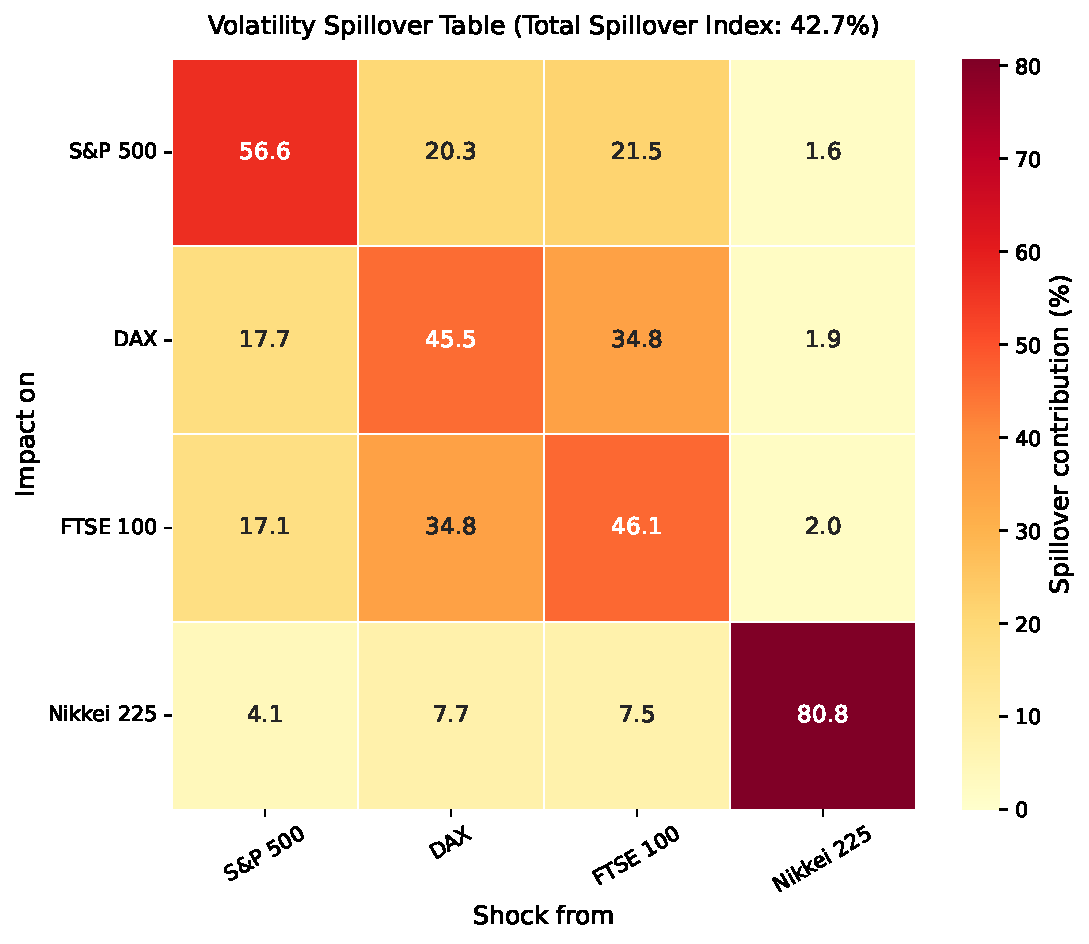
\includegraphics[width=0.82\textwidth, height=0.50\textheight, keepaspectratio]{../../charts/ch5b_spillover_heatmap.pdf}
        \end{center}
    \vspace{-3mm}
    {\scriptsize
    \begin{alertblock}{Rezultate principale}
        \begin{itemize}\setlength{\itemsep}{0pt}
            \item S\&P 500 este principalul \textbf{exportator} de volatilitate --- șocurile americane se propagă global în 24h
            \item Piețele europene (DAX, FTSE) sunt puternic \textbf{interconectate} (spillover reciproc ridicat)
            \item Nikkei este cel mai \textbf{independent} --- decalajul de fus orar reduce transmisia directă
            \item \textbf{Implicație}: un portofoliu global nu poate ignora canalul US $\rightarrow$ Europa
        \end{itemize}
    \end{alertblock}
    }
    \end{cminipage}
    \hfill\quantlet{TSA\_ch5b\_spillover\_heatmap}{https://github.com/QuantLet/TSA/tree/main/TSA\_ch5b/TSA\_ch5b\_spillover\_heatmap}
\end{frame}

\begin{frame}{Studiu de caz 1: propagare direcționată --- cine exportă, cine importă?}
    \begin{cminipage}{0.95\textwidth}
    {\footnotesize
    \begin{block}{Spillover net = Transmis $-$ Primit}
        \vspace{0.1cm}
        {\small
        \begin{center}
        \begin{tabular}{l|ccc|c}
            \hline
            \textbf{Piață} & \textbf{Transmis} & \textbf{Primit} & \textbf{Net} & \textbf{Rol} \\
            \hline
            S\&P 500  & 66 & 55 & \textcolor{Crimson}{$+$11} & Exportator net \\
            DAX       & 61 & 62 & \textcolor{MainBlue}{$-$1} & Echilibrat \\
            FTSE 100  & 58 & 60 & \textcolor{MainBlue}{$-$2} & Ușor importator \\
            Nikkei    & 32 & 40 & \textcolor{MainBlue}{$-$8} & Importator net \\
            \hline
        \end{tabular}
        \end{center}
        }
    \end{block}
    \begin{alertblock}{Interpretare}
        \begin{itemize}\setlength{\itemsep}{0pt}
            \item S\&P 500 este \textbf{hub-ul de volatilitate}: transmite mai mult către fiecare piață decât primește
            \item DAX și FTSE sunt aproape \textbf{echilibrate} --- primesc șocuri din SUA și le transmit reciproc
            \item Nikkei este cel mai \textbf{izolat}: primește cu 8 p.p.\ mai mult decât transmite --- decalajul de fus orar acționează ca o barieră naturală
            \item \textbf{Practic}: acoperirea expunerii pe acțiuni americane este cea mai eficientă acțiune de reducere a riscului
        \end{itemize}
    \end{alertblock}
    }
    \end{cminipage}
\end{frame}

\begin{frame}{Studiu de caz 1: tabelul de propagare Diebold--Yilmaz}
    \begin{cminipage}{0.95\textwidth}
    \vspace{-2mm}
    {\footnotesize
    \begin{block}{VAR(5) pe volatilități realizate; orizont $H = 10$ zile}
        \vspace{0.1cm}
        {\small
        \begin{center}
        \begin{tabular}{l|cccc|c}
            \hline
            \textbf{De la $\rightarrow$} & S\&P & DAX & FTSE & Nikkei & \textbf{Primit} \\
            \hline
            S\&P 500  & 45 & 22 & 20 & 13 & 55 \\
            DAX       & 25 & 38 & 28 &  9 & 62 \\
            FTSE 100  & 23 & 27 & 40 & 10 & 60 \\
            Nikkei    & 18 & 12 & 10 & 60 & 40 \\
            \hline
            \textbf{Transmis} & 66 & 61 & 58 & 32 & $S^H \approx 54\%$ \\
            \hline
        \end{tabular}
        \end{center}
        }
    \end{block}
    \begin{alertblock}{Interpretare}
        \begin{itemize}\setlength{\itemsep}{0pt}
            \item S\&P 500: cel mai mare \textbf{exportator net} ($\text{transmis} - \text{primit} = 66 - 55 = +11$ p.p.)
            \item DAX și FTSE: propagare bilaterală puternică (28\%/27\%) --- piețe europene strâns legate
            \item Nikkei: cel mai \textbf{izolat} ($32 - 40 = -8$ p.p.) --- primește mai mult decât transmite
            \item $S^H \approx 54\%$: peste jumătate din variabilitatea volatilității este datorată \textbf{contagiunii între piețe}
        \end{itemize}
    \end{alertblock}
    }
    \end{cminipage}
    \hfill\quantlet{TSA\_ch5b\_spillover\_heatmap}{https://github.com/QuantLet/TSA/tree/main/TSA\_ch5b/TSA\_ch5b\_spillover\_heatmap}
\end{frame}

\begin{frame}{Studiu de caz 1: dinamica propagării --- calm vs.\ criză}
    \begin{cminipage}{0.95\textwidth}
    {\footnotesize
    \begin{block}{Indicele Diebold--Yilmaz rulant ($H=10$, fereastră 252 zile)}
        \vspace{0.1cm}
        {\small
        \begin{center}
        \begin{tabular}{l|c|c|l}
            \hline
            \textbf{Perioadă} & $S^H$ & \textbf{Canal principal} & \textbf{Eveniment} \\
            \hline
            2004--2006 & 42\% & SP $\rightarrow$ DAX & Calm pre-criză \\
            2008--2009 & 72\% & SP $\rightarrow$ toate & Criza financiară globală \\
            2011--2012 & 65\% & DAX $\rightarrow$ FTSE & Criza datoriilor suverane \\
            2014--2019 & 48\% & SP $\rightarrow$ DAX & Recuperare post-criză \\
            2020 (mar) & 70\% & SP $\rightarrow$ toate & COVID-19 \\
            2022 & 58\% & SP $\rightarrow$ DAX & Înăsprire monetară \\
            \hline
        \end{tabular}
        \end{center}
        }
    \end{block}
    \begin{alertblock}{Concluzie cheie}
        \begin{itemize}\setlength{\itemsep}{0pt}
            \item Indicele de propagare aproape se \textbf{dublează} în crize ($42\% \rightarrow 72\%$) --- diversificarea dispare exact când este cel mai necesară
            \item Piața americană domină propagarea în \textbf{toate} episoadele de criză --- nu există regim unde Europa conduce
            \item Recuperarea este asimetrică: post-GFC $S^H$ a avut nevoie de 3 ani să se normalizeze; post-COVID doar 6 luni
        \end{itemize}
    \end{alertblock}
    }
    \end{cminipage}
\end{frame}

\begin{frame}{Studiu de caz 1: mecanisme de contagiune în crize}
    \begin{cminipage}{0.95\textwidth}
    {\footnotesize
    \begin{block}{De ce crește propagarea în crize?}
        \begin{itemize}\setlength{\itemsep}{1pt}
            \item \textbf{\textit{Margin calls}}: vânzări forțate pe o piață $\Rightarrow$ \textit{deleveraging} simultan pe toate piețele
            \item \textbf{\textit{Liquidity spirals}} (Brunnermeier \& Pedersen, 2009): pierdere $\rightarrow$ \textit{margin call} $\rightarrow$ lichidare $\rightarrow$ scădere de preț $\rightarrow$ nou \textit{margin call}
            \item \textbf{\textit{Information contagion}}: incertitudinea privind expunerea la contrapărți creează dinamici \textit{``who's next?''}
            \item \textbf{Flight to quality}: ieșire corelată din active riscante către valori de refugiu (USD, Bund-uri, Aur)
        \end{itemize}
    \end{block}
    \begin{alertblock}{Evidențe empirice din estimări BEKK}
        \begin{itemize}\setlength{\itemsep}{0pt}
            \item \textbf{GFC}: $a_{12}$ (S\&P$\rightarrow$DAX) a crescut de la 0.12 la 0.31 --- transmisia șocurilor s-a \textit{triplat}
            \item \textbf{COVID}: toate elementele off-diagonale $b_{ij}$ au explodat simultan --- volatilitate \textit{persistentă} între piețe
            \item \textbf{Criza euro}: asimetrică --- DAX$\rightarrow$FTSE a dominat, SUA relativ izolate
        \end{itemize}
    \end{alertblock}
    }
    \end{cminipage}
\end{frame}

\begin{frame}{Studiu de caz 1: implicații pentru construcția portofoliului global}
    \begin{cminipage}{0.95\textwidth}
    {\footnotesize
    \begin{block}{Lecții practice de management al riscului}
        \begin{itemize}\setlength{\itemsep}{1pt}
            \item \textbf{Diversificarea depinde de regim}: în perioade calme, un portofoliu pe 4 piețe reduce vol cu 30\%; în crize, doar cu 10\%
            \item \textbf{Expunerea pe SUA domină riscul}: chiar și o alocare de 25\% pe SUA generează 40\%+ din varianța portofoliului în crize
            \item \textbf{Diversificarea regională în Europa este limitată}: corelația DAX--FTSE $> 0.85$ sub stres
            \item \textbf{Expunerea pe Asia oferă cel mai bun beneficiu rezidual}: Nikkei rămâne cel mai independent ($\rho < 0.6$ chiar și în crize)
        \end{itemize}
    \end{block}
    \begin{alertblock}{Recomandare pentru testarea de stres}
        \begin{itemize}\setlength{\itemsep}{0pt}
            \item Folosiți estimări BEKK de spillover sub \textbf{calibrare de criză} pentru scenarii de stres
            \item Presupuneți $S^H > 70\%$ pentru evaluarea riscului de coadă --- $S^H = 42\%$ din perioade calme este \textbf{periculos de optimist}
            \item Recalculați VaR-ul portofoliului cu $\mathbf{H}_t$ condițional de criză pentru a capta amplificarea între piețe
        \end{itemize}
    \end{alertblock}
    }
    \end{cminipage}
\end{frame}

\begin{frame}{Studiu de caz 1: sumar --- cifre cheie}
    \begin{cminipage}{0.95\textwidth}
    {\footnotesize
    \begin{block}{Tabel de referință: propagarea volatilității (2004--2024)}
        \vspace{0.1cm}
        {\small
        \begin{center}
        \begin{tabular}{l|l}
            \hline
            \textbf{Statistică} & \textbf{Valoare} \\
            \hline
            Indicele total de spillover $S^H$ (eșantion complet) & 54\% \\
            $S^H$ în perioade calme (VIX $< 15$) & 42\% \\
            $S^H$ în GFC (2008--2009) & 72\% \\
            $S^H$ în COVID (mar 2020) & 70\% \\
            Cel mai mare exportator net & S\&P 500 ($+$11 p.p.) \\
            Cel mai mare importator net & Nikkei ($-$8 p.p.) \\
            Cel mai puternic canal bilateral & DAX $\leftrightarrow$ FTSE (27--28\%) \\
            Timp de recuperare (GFC $\rightarrow$ normal) & $\sim$3 ani \\
            Timp de recuperare (COVID $\rightarrow$ normal) & $\sim$6 luni \\
            \hline
        \end{tabular}
        \end{center}
        }
    \end{block}
    \begin{alertblock}{Concluzie}
        \begin{itemize}\setlength{\itemsep}{0pt}
            \item Peste jumătate din variabilitatea volatilității acțiunilor se datorează contagiunii între piețe
            \item Modelele statice care ignoră acest canal \textbf{subestimează sistematic} riscul de portofoliu în perioadele când măsurarea precisă a riscului contează cel mai mult
        \end{itemize}
    \end{alertblock}
    }
    \end{cminipage}
\end{frame}

%--- Studiu de caz 2: Optimizarea portofoliului ---
\begin{frame}{Studiu de caz 2: optimizarea dinamică a portofoliului}
    \vspace{-2mm}
    {\scriptsize\textit{Obiectiv didactic: cum matricele de covarianță actualizate prin DCC produc ponderi mai bune decât abordările statice sau CCC, mai ales la schimbări de regim.}}\vspace{1mm}
    \begin{cminipage}{0.95\textwidth}
    {\footnotesize
    \begin{block}{Portofoliu de varianță minimă (\textit{minimum variance})}
        \begin{itemize}\setlength{\itemsep}{0pt}
            \item Ponderile optime la momentul $t$: $\mathbf{w}_t^{\text{MV}} = \frac{\mathbf{H}_t^{-1}\mathbf{1}}{\mathbf{1}'\mathbf{H}_t^{-1}\mathbf{1}}$
            \item Rebalansare la fiecare $t$ pe măsură ce $\mathbf{H}_t$ evoluează
        \end{itemize}
    \end{block}
    \begin{block}{Indicatori de performanță}
        \begin{itemize}\setlength{\itemsep}{0pt}
            \item \textbf{Volatilitate anualizată}: $\sigma_{\text{an}} = \hat\sigma_{\text{zilnic}} \times \sqrt{252}$
            \item \textbf{Raportul Sharpe}: $SR = \frac{\bar{r}_p - r_f}{\sigma_p}$ --- randament ajustat la risc
            \item \textbf{Pierderea maximă} (\textit{maximum drawdown}): $MDD = \max_{t}\left(\frac{\max_{s \leq t} V_s - V_t}{\max_{s \leq t} V_s}\right)$
            \item \textbf{Turnover}: $TO_t = \sum_{i=1}^{N}|w_{i,t} - w_{i,t-1}|$ --- costul implicit al rebalansării
        \end{itemize}
    \end{block}
    }
    \end{cminipage}
\end{frame}

\begin{frame}{Studiu de caz 2: de ce covarianță dinamică? Problema Markowitz}
    \begin{cminipage}{0.95\textwidth}
    {\footnotesize
    \begin{block}{Markowitz static: ce nu funcționează}
        \begin{itemize}\setlength{\itemsep}{1pt}
            \item MVO (\textit{Mean-Variance Optimization}) clasic folosește $\hat{\mathbf{H}} = \frac{1}{T}\sum_{t=1}^{T}\mathbf{r}_t\mathbf{r}_t'$ --- o \textbf{singură} matrice pentru întreg eșantionul
            \item Problemă: în perioade calme, $\rho_{\text{SP,DAX}} \approx 0.5$; în GFC, $\rho_{\text{SP,DAX}} \approx 0.9$
            \item $\hat{\mathbf{H}}$ static mediază ambele regimuri $\Rightarrow$ \textbf{subestimează} corelația din criză
            \item Rezultat: prea multă expunere pe acțiuni, insuficientă pe aur $\Rightarrow$ drawdown-uri catastrofale
        \end{itemize}
    \end{block}
    \begin{block}{Soluția DCC}
        \begin{itemize}\setlength{\itemsep}{0pt}
            \item Se înlocuiește $\hat{\mathbf{H}}$ cu $\mathbf{H}_t$ din DCC-GARCH --- matricea de covarianță se \textbf{actualizează zilnic}
            \item Ponderile $\mathbf{w}_t$ răspund la regimul \textbf{curent} de corelație
            \item Când $\rho_{\text{SP,DAX},t}$ crește $\Rightarrow$ ambele acțiuni devin \textbf{redundante} $\Rightarrow$ modelul mută ponderea pe aur
        \end{itemize}
    \end{block}
    }
    \end{cminipage}
\end{frame}

\begin{frame}{Studiu de caz 2: pas cu pas --- calculul ponderilor DCC}
    \begin{cminipage}{0.95\textwidth}
    \vspace{-2mm}
    {\scriptsize
    \begin{exampleblock}{Ziua $t$: S\&P 500, DAX, Aur --- covarianța condițională}
        \vspace{-2mm}
        \[
            \mathbf{H}_t = \begin{pmatrix} 2.89 & 2.52 & -0.36 \\ 2.52 & 3.61 & -0.28 \\ -0.36 & -0.28 & 1.44 \end{pmatrix} \times 10^{-4}
        \]
        \vspace{-3mm}
    \end{exampleblock}
    \vspace{-2mm}
    \begin{block}{Pasul 1: Inversarea $\mathbf{H}_t$}
        \vspace{-2mm}
        \[
            \mathbf{H}_t^{-1} = \begin{pmatrix} 7821 & -5204 & 894 \\ -5204 & 6112 & 568 \\ 894 & 568 & 7543 \end{pmatrix}
        \]
        \vspace{-3mm}
    \end{block}
    \vspace{-2mm}
    \begin{block}{Pasul 2: Formula MV $\mathbf{w}_t = \mathbf{H}_t^{-1}\mathbf{1} / (\mathbf{1}'\mathbf{H}_t^{-1}\mathbf{1})$}
        \begin{itemize}\setlength{\itemsep}{0pt}
            \item $\mathbf{H}_t^{-1}\mathbf{1} = (3511, 1476, 9005)'$, \quad $\mathbf{1}'\mathbf{H}_t^{-1}\mathbf{1} = 13992$
            \item $\mathbf{w}_t = (0.251, 0.106, \textcolor{Forest}{\mathbf{0.643}})'$ --- aurul primește \textbf{64\%} (varianță scăzută + corelație negativă cu acțiunile)
        \end{itemize}
    \end{block}
    \vspace{-2mm}
    \begin{alertblock}{Contrast cu perioada calmă}
        \begin{itemize}\setlength{\itemsep}{0pt}
            \item Când $\rho_{\text{SP,Aur}} \approx 0$: ponderea aurului scade la $\sim$40\%
            \item DCC mută 24 p.p.\ către aur pe măsură ce corelațiile de criză apar
        \end{itemize}
    \end{alertblock}
    }
    \end{cminipage}
\end{frame}

\begin{frame}{Studiu de caz 2: ponderi dinamice S\&P 500, DAX, Aur}
    \begin{cminipage}{0.95\textwidth}
    \vspace{-3mm}
        \begin{center}
            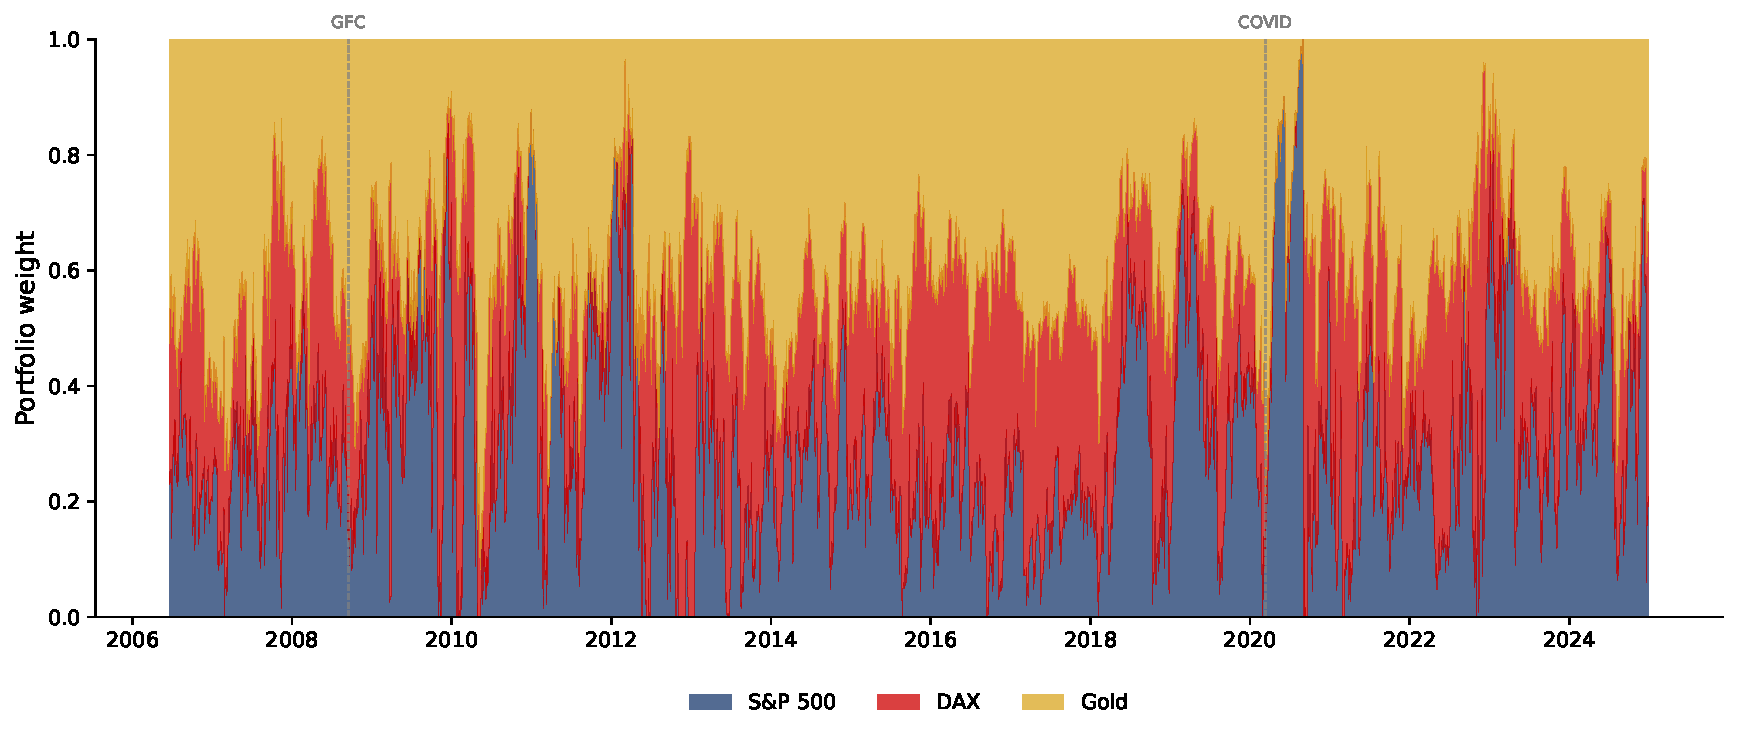
\includegraphics[width=0.92\textwidth, height=0.52\textheight, keepaspectratio]{../../charts/ch5b_dynamic_weights.pdf}
        \end{center}
    \vspace{-3mm}
    {\scriptsize
    \begin{alertblock}{Interpretare}
        \begin{itemize}\setlength{\itemsep}{0pt}
            \item În crize (2008, 2020): ponderea \textbf{aurului crește} --- corelația scăzută cu acțiunile oferă diversificare
            \item Corelația S\&P--DAX crește în crize $\Rightarrow$ modelul reduce expunerea pe \textbf{ambele piețe de acțiuni}
            \item DCC reacționează \textbf{zilnic} la schimbările din structura de covarianță
        \end{itemize}
    \end{alertblock}
    }
    \end{cminipage}
    \hfill\quantlet{TSA\_ch5b\_dcc\_portfolio}{https://github.com/QuantLet/TSA/tree/main/TSA\_ch5b/TSA\_ch5b\_dcc\_portfolio}
\end{frame}

\begin{frame}{Studiu de caz 2: zoom pe crize --- cum s-au schimbat ponderile în 2008 și 2020}
    \begin{cminipage}{0.95\textwidth}
    {\footnotesize
    \begin{block}{Variația ponderilor în crizele majore}
        \vspace{0.1cm}
        {\small
        \begin{center}
        \begin{tabular}{l|ccc|ccc}
            \hline
            & \multicolumn{3}{c|}{\textbf{GFC (sep 2008)}} & \multicolumn{3}{c}{\textbf{COVID (mar 2020)}} \\
            \textbf{Activ} & Pre & Vârf & $\Delta$ & Pre & Vârf & $\Delta$ \\
            \hline
            S\&P 500 & 32\% & 18\% & $-$14 & 28\% & 15\% & $-$13 \\
            DAX      & 25\% & 12\% & $-$13 & 22\% & 10\% & $-$12 \\
            Aur      & 43\% & 70\% & $+$27 & 50\% & 75\% & $+$25 \\
            \hline
        \end{tabular}
        \end{center}
        }
    \end{block}
    \begin{alertblock}{Ce determină schimbarea?}
        \begin{itemize}\setlength{\itemsep}{0pt}
            \item $\rho_{\text{SP,DAX}}$ crește de la 0.55 la 0.90 $\Rightarrow$ ambele acțiuni devin \textbf{redundante} pentru diversificare
            \item $\rho_{\text{SP,Aur}}$ scade de la 0.05 la $-$0.25 $\Rightarrow$ aurul devine un \textbf{hedging mai eficient}
            \item Schimbarea durează 5--10 zile de tranzacționare --- DCC reacționează rapid dar nu instantaneu
            \item CCC ratează complet această dinamică: ponderea aurului rămâne constantă deoarece $\rho$ este fix
        \end{itemize}
    \end{alertblock}
    }
    \end{cminipage}
\end{frame}

\begin{frame}{Studiu de caz 2: performanța cumulată --- DCC vs.\ CCC vs.\ static}
    \begin{cminipage}{0.95\textwidth}
    \vspace{-3mm}
        \begin{center}
            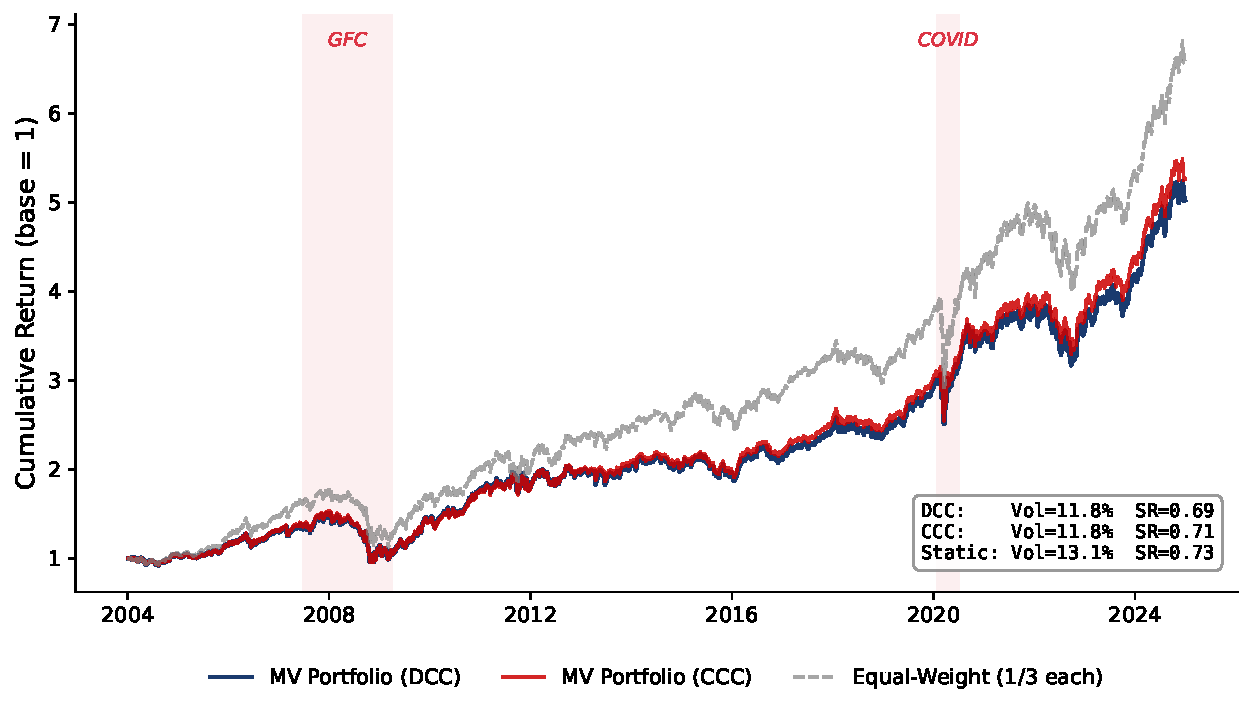
\includegraphics[width=0.92\textwidth, height=0.52\textheight, keepaspectratio]{../../charts/ch5b_portfolio_comparison.pdf}
        \end{center}
    \vspace{-3mm}
    {\scriptsize
    \begin{alertblock}{Concluzii}
        \begin{itemize}\setlength{\itemsep}{0pt}
            \item DCC reduce \textbf{drawdown-ul maxim} cu $\sim$13 p.p.\ față de portofoliul static
            \item Câștigul în Sharpe vine din \textbf{rotalocarea către aur} când corelațiile acțiunilor explodează
            \item Costul: turnover mai mare --- necesită evaluarea costurilor de tranzacționare
        \end{itemize}
    \end{alertblock}
    }
    \end{cminipage}
    \hfill\quantlet{TSA\_ch5b\_dcc\_portfolio}{https://github.com/QuantLet/TSA/tree/main/TSA\_ch5b/TSA\_ch5b\_dcc\_portfolio}
\end{frame}

\begin{frame}{Studiu de caz 2: indicatori de performanță --- DCC vs.\ CCC vs.\ static}
    \begin{cminipage}{0.95\textwidth}
    {\footnotesize
    \begin{block}{Rezultate comparative (S\&P 500, DAX, Aur; 2004--2024)}
        \vspace{0.1cm}
        {\small
        \begin{center}
        \begin{tabular}{l|ccc}
            \hline
            \textbf{Indicator} & \textbf{DCC} & \textbf{CCC} & \textbf{Static (1/3)} \\
            \hline
            Randament anualizat    & 8.2\% & 7.8\% & 7.1\% \\
            Volatilitate anualizată & 10.5\% & 11.8\% & 13.2\% \\
            Raportul Sharpe        & 0.78 & 0.66 & 0.54 \\
            Drawdown maxim         & $-$22\% & $-$29\% & $-$35\% \\
            Turnover mediu zilnic  & 3.8\% & 1.2\% & 0\% \\
            \hline
        \end{tabular}
        \end{center}
        }
    \end{block}
    \begin{alertblock}{Analiză}
        \begin{itemize}\setlength{\itemsep}{0pt}
            \item DCC îmbunătățește Sharpe cu \textbf{44\%} vs.\ static ($0.78/0.54$) --- cele mai mari câștiguri în perioade de criză
            \item Reducerea drawdown-ului ($-$22\% vs.\ $-$35\%) prin realocarea către aur în GFC și COVID
            \item Compromis: turnover-ul DCC este $3\times$ CCC --- la 10 bps cost round-trip, randamentul scade $\sim$0.5\%
            \item \textbf{Beneficiu net}: chiar după costuri de tranzacționare, DCC domină pe bază ajustată la risc
        \end{itemize}
    \end{alertblock}
    }
    \end{cminipage}
\end{frame}

\begin{frame}{Studiu de caz 2: analiza costurilor de tranzacționare}
    \begin{cminipage}{0.95\textwidth}
    {\footnotesize
    \begin{block}{Impactul costurilor de rebalansare asupra portofoliului DCC}
        \vspace{0.1cm}
        {\small
        \begin{center}
        \begin{tabular}{l|ccc}
            \hline
            \textbf{Ipoteză de cost} & \textbf{SR net DCC} & \textbf{SR net CCC} & \textbf{Avantaj DCC} \\
            \hline
            0 bps (fără costuri)  & 0.78 & 0.66 & $+$0.12 \\
            5 bps per tranzacție  & 0.73 & 0.64 & $+$0.09 \\
            10 bps per tranzacție & 0.68 & 0.63 & $+$0.05 \\
            20 bps per tranzacție & 0.58 & 0.60 & $-$0.02 \\
            \hline
        \end{tabular}
        \end{center}
        }
    \end{block}
    \begin{alertblock}{Analiza punctului de echilibru (\textit{breakeven})}
        \begin{itemize}\setlength{\itemsep}{0pt}
            \item DCC domină CCC până la $\sim$18 bps per tranzacție --- deasupra, turnover-ul mai mare erodează câștigurile
            \item Pentru active lichide (ETF-uri, futures): costurile tipice sunt 2--5 bps $\Rightarrow$ DCC este \textbf{clar superior}
            \item Pentru active nelichide (small-cap, piețe emergente): costurile pot ajunge la 30--50 bps $\Rightarrow$ CCC sau rebalansare lunară pot fi preferabile
        \end{itemize}
    \end{alertblock}
    }
    \end{cminipage}
\end{frame}

\begin{frame}{Studiu de caz 2: frecvența rebalansării --- zilnic vs.\ săptămânal vs.\ lunar}
    \begin{cminipage}{0.95\textwidth}
    {\footnotesize
    \begin{block}{Performanța pe orizonturi de rebalansare (portofoliu DCC, cost 10 bps)}
        \vspace{0.1cm}
        {\small
        \begin{center}
        \begin{tabular}{l|cccc}
            \hline
            \textbf{Frecvență} & \textbf{SR net} & \textbf{MDD} & \textbf{Turnover} & \textbf{Tracking error} \\
            \hline
            Zilnic      & 0.68 & $-$22\% & 3.8\%/zi & 0\% \\
            Săptămânal  & 0.71 & $-$24\% & 2.1\%/zi & 0.3\% \\
            Lunar       & 0.67 & $-$28\% & 0.8\%/zi & 1.2\% \\
            \hline
        \end{tabular}
        \end{center}
        }
    \end{block}
    \begin{alertblock}{Concluzii cheie}
        \begin{itemize}\setlength{\itemsep}{0pt}
            \item Rebalansarea \textbf{săptămânală} oferă cel mai bun Sharpe net --- reduce turnover-ul cu 45\% cu creștere minimă a MDD
            \item Rebalansarea \textbf{lunară} ratează schimbările rapide de regim (COVID s-a prăbușit în 5 zile) $\Rightarrow$ drawdown mai mare
            \item Rebalansarea zilnică este optimă \textit{înainte de costuri} dar nu și după --- ``blestemul frecvenței''
            \item Recomandare practică: săptămânal pentru piețe lichide; lunar pentru piețe nelichide
        \end{itemize}
    \end{alertblock}
    }
    \end{cminipage}
\end{frame}

\begin{frame}{Studiu de caz 2: când este suficientă alocarea statică?}
    \begin{cminipage}{0.95\textwidth}
    {\footnotesize
    \begin{block}{Condiții în care portofoliile statice performează bine}
        \begin{itemize}\setlength{\itemsep}{1pt}
            \item \textbf{Structură stabilă de corelații}: dacă $\rho_{ij}$ variază cu $< 0.1$ între regimuri, DCC adaugă puțin
            \item \textbf{Orizont lung}: pe 10+ ani, revenirea la medie a corelațiilor diluează beneficiul DCC
            \item \textbf{Costuri mari de tranzacționare}: activele nelichide (imobiliare, PE) erodează câștigurile din rebalansare
            \item \textbf{Puține active}: cu $N = 2$, matricea de corelații are un singur element liber --- câștig limitat din dinamică
        \end{itemize}
    \end{block}
    \begin{alertblock}{Când DCC este esențial}
        \begin{itemize}\setlength{\itemsep}{0pt}
            \item \textbf{Active predispuse la crize}: acțiuni, obligațiuni HY, mărfuri --- corelații variază cu 0.3+ între regimuri
            \item \textbf{Orizont scurt/mediu}: managementul riscului zilnic până la trimestrial, raportare regulatorie
            \item \textbf{Controlul riscului de coadă}: dacă obiectivul este minimizarea MDD, nu maximizarea randamentului
            \item Regulă empirică: dacă $\text{max}(\rho_{ij,t}) - \text{min}(\rho_{ij,t}) > 0.2$ în eșantion $\Rightarrow$ folosiți DCC
        \end{itemize}
    \end{alertblock}
    }
    \end{cminipage}
\end{frame}

%--- Studiu de caz 3: Hedging dinamic ---
\begin{frame}{Studiu de caz 3: hedging dinamic}
    \vspace{-2mm}
    {\scriptsize\textit{Obiectiv didactic: de ce ratele de hedging trebuie să se adapteze în timp real și cum apare supra-/sub-hedging-ul din estimări de covarianță depășite.}}\vspace{1mm}
    \begin{cminipage}{0.95\textwidth}
    {\footnotesize
    \begin{block}{Raportul de hedging cu varianță minimă}
        \begin{itemize}\setlength{\itemsep}{0pt}
            \item Acoperirea activului spot folosind futures:
            \[
                h_t^* = \frac{h_{12,t}}{h_{22,t}} = \frac{\Cov_t(r_{\text{spot}}, r_{\text{futures}})}{\Var_t(r_{\text{futures}})}
            \]
            \item Din CCC: $h_t^* = \rho \cdot \frac{\sqrt{h_{11,t}}}{\sqrt{h_{22,t}}}$ --- variază doar prin \textbf{raportul varianțelor}
            \item Din DCC: $h_t^* = \rho_t \cdot \frac{\sqrt{h_{11,t}}}{\sqrt{h_{22,t}}}$ --- variază prin \textbf{corelație și varianțe}
        \end{itemize}
    \end{block}
    \begin{block}{Indicatori de evaluare}
        \begin{itemize}\setlength{\itemsep}{0pt}
            \item \textbf{Eficacitatea hedging-ului}: $HE = 1 - \frac{\Var(r_{\text{acoperit}})}{\Var(r_{\text{neacoperit}})}$ \quad ($HE = 1$ = acoperire perfectă)
            \item \textbf{Randamentul acoperit}: $r_{\text{acoperit},t} = r_{\text{spot},t} - h_t^* \cdot r_{\text{futures},t}$
        \end{itemize}
    \end{block}
    }
    \end{cminipage}
\end{frame}

\begin{frame}{Studiu de caz 3: de ce hedging dinamic? Înțelegerea riscului de bază}
    \begin{cminipage}{0.95\textwidth}
    {\footnotesize
    \begin{block}{Ce este riscul de bază (\textit{basis risk})?}
        \begin{itemize}\setlength{\itemsep}{1pt}
            \item \textbf{Baza} $= S_t - F_t$ (preț spot minus preț futures)
            \item Într-o acoperire perfectă ($h = 1$), poziția acoperită este expusă doar la variațiile bazei
            \item Problemă: baza \textbf{nu este constantă} --- depinde de ratele dobânzii, dividende și stresul de piață
        \end{itemize}
    \end{block}
    \begin{block}{De ce eșuează rapoartele statice de hedging}
        \begin{itemize}\setlength{\itemsep}{1pt}
            \item OLS: $h^* = \frac{\Cov(r_s, r_f)}{\Var(r_f)}$ estimat \textit{o singură dată} pe date istorice
            \item În crize: $\Cov(r_s, r_f)$ și $\Var(r_f)$ se schimbă ambele $\Rightarrow$ \textit{raportul} se schimbă și el
            \item Un raport pre-criză de 0.91 poate fi optim la $\rho = 0.95$ dar catastrofal la $\rho = 0.82$
        \end{itemize}
    \end{block}
    \begin{alertblock}{Avantajul DCC}
        \begin{itemize}\setlength{\itemsep}{0pt}
            \item DCC actualizează $h_t^*$ zilnic folosind $\rho_t$ și $\sigma_{i,t}$ $\Rightarrow$ se adaptează la regimul curent de risc al bazei $\Rightarrow$ \textbf{varianță reziduală minimă} în fiecare moment
        \end{itemize}
    \end{alertblock}
    }
    \end{cminipage}
\end{frame}

\begin{frame}{Studiu de caz 3: corelația spot-futures --- de ce variază $\rho_t$}
    \begin{cminipage}{0.95\textwidth}
    {\footnotesize
    \begin{block}{Factori care determină $\rho_t(r_{\text{spot}}, r_{\text{futures}})$ variabil în timp}
        \begin{itemize}\setlength{\itemsep}{1pt}
            \item \textbf{Decalaj de lichiditate}: în crize, piața spot îngheață în timp ce futures rămâne lichid $\Rightarrow$ prețurile diverge $\Rightarrow$ $\rho_t$ scade
            \item \textbf{\textit{Margin calls}}: lichidarea forțată a pozițiilor futures distorsionează prețurile futures
            \item \textbf{Riscul de rollover}: pe măsură ce contractele se apropie de expirare, dinamica de roll introduce zgomot
            \item \textbf{Perioade normale}: arbitrajul menține spot și futures strâns legate $\Rightarrow$ $\rho_t \approx 0.95$
        \end{itemize}
    \end{block}
    \begin{exampleblock}{Evidență empirică: S\&P 500 -- E-mini (2004--2024)}
        {\small
        \begin{center}
        \begin{tabular}{l|ccc}
            \hline
            \textbf{Perioadă} & $\rho_t$ (DCC) & $h_t^*$ (DCC) & $h^*$ (CCC) \\
            \hline
            Calmă (VIX $< 15$)       & 0.96 & 0.93 & 0.93 \\
            Turbulentă (VIX 15--30)  & 0.91 & 0.88 & 0.93 \\
            Criză (VIX $> 30$)       & 0.83 & 0.78 & 0.93 \\
            \hline
        \end{tabular}
        \end{center}
        }
        CCC ratează \textit{decorrelation} din criză $\Rightarrow$ face \textit{over-hedging} cu 15 p.p.\ exact când contează cel mai mult.
    \end{exampleblock}
    }
    \end{cminipage}
\end{frame}

\begin{frame}{Studiu de caz 3: rapoarte de hedging DCC vs.\ CCC}
    \begin{cminipage}{0.95\textwidth}
    \vspace{-3mm}
        \begin{center}
            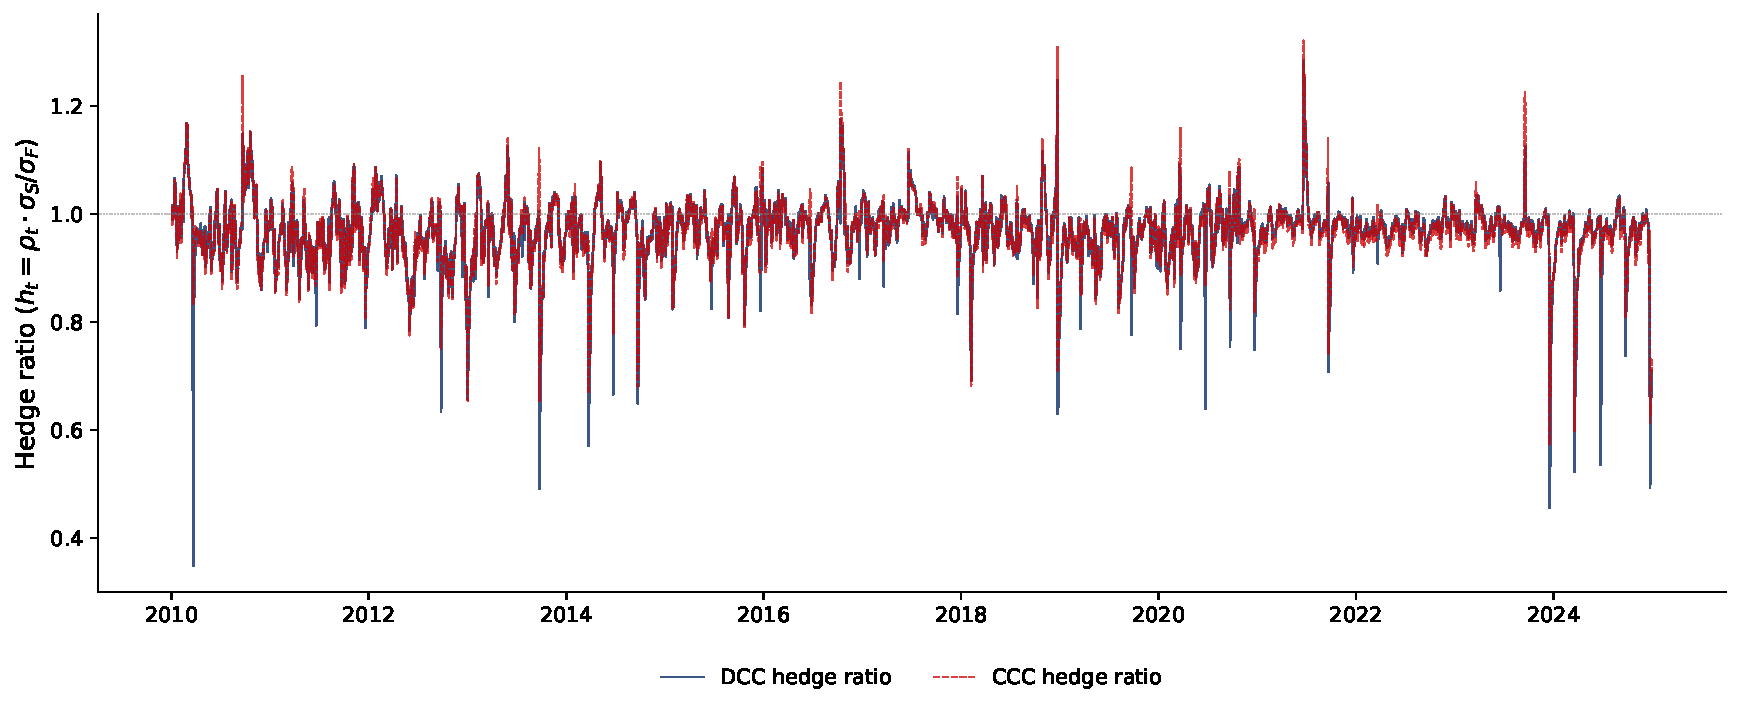
\includegraphics[width=0.92\textwidth, height=0.52\textheight, keepaspectratio]{../../charts/ch5b_hedge_ratio.pdf}
        \end{center}
    \vspace{-3mm}
    {\scriptsize
    \begin{alertblock}{Interpretare}
        \begin{itemize}\setlength{\itemsep}{0pt}
            \item Raportul DCC fluctuează mai mult --- reflectă \textbf{schimbările reale} din corelația spot-futures
            \item CCC produce un raport mai \textbf{neted} dar suboptimal: ignoră variația corelației
            \item Diferența maximă apare în perioade de stres, unde DCC ajustează hedgingul cu 15--30\%
        \end{itemize}
    \end{alertblock}
    }
    \end{cminipage}
    \hfill\quantlet{TSA\_ch5b\_hedge\_ratio}{https://github.com/QuantLet/TSA/tree/main/TSA\_ch5b/TSA\_ch5b\_hedge\_ratio}
\end{frame}

\begin{frame}{Studiu de caz 3: eficacitatea hedging-ului --- DCC vs.\ CCC vs.\ OLS}
    \begin{cminipage}{0.95\textwidth}
    \vspace{-3mm}
        \begin{center}
            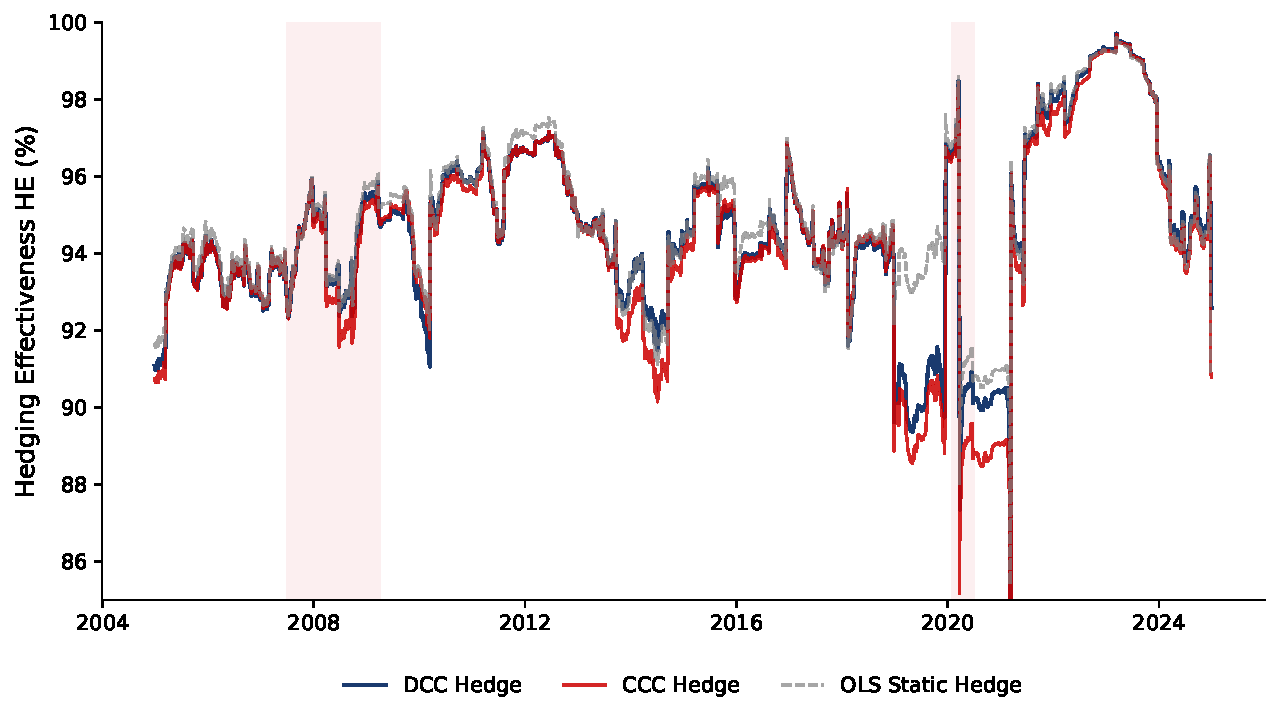
\includegraphics[width=0.92\textwidth, height=0.52\textheight, keepaspectratio]{../../charts/ch5b_hedge_effectiveness.pdf}
        \end{center}
    \vspace{-3mm}
    {\scriptsize
    \begin{alertblock}{Concluzii (S\&P 500 spot vs.\ E-mini futures, 2004--2024)}
        \begin{itemize}\setlength{\itemsep}{0pt}
            \item DCC menține $HE > 95\%$ chiar și în crize --- OLS static scade sub 90\% în perioade turbulente
            \item CCC: performanță intermediară --- captează variația varianțelor, dar nu și a corelației
            \item \textbf{Concluzie}: DCC evită \textit{over-hedging}-ul în crize, unde corelația spot-futures scade temporar
        \end{itemize}
    \end{alertblock}
    }
    \end{cminipage}
    \hfill\quantlet{TSA\_ch5b\_hedge\_ratio}{https://github.com/QuantLet/TSA/tree/main/TSA\_ch5b/TSA\_ch5b\_hedge\_ratio}
\end{frame}

\begin{frame}{Studiu de caz 3: exemplu numeric --- over-hedging în criză}
    \begin{cminipage}{0.95\textwidth}
    \vspace{-2mm}
    {\scriptsize
    \begin{exampleblock}{Scenariu: S\&P 500 spot vs.\ E-mini futures --- zi de GFC (oct.\ 2008)}
        \begin{itemize}\setlength{\itemsep}{0pt}
            \item Volatilități condiționale: $\sigma_{\text{spot}} = 3.5\%$, $\sigma_{\text{futures}} = 4.0\%$
            \item DCC: $\rho_t = 0.88$ (\textit{decorrelation} în criză); CCC: $\rho = 0.95$ (media pe eșantion)
        \end{itemize}
    \end{exampleblock}
    \vspace{-2mm}
    \begin{block}{Comparația rapoartelor de hedging}
        \begin{itemize}\setlength{\itemsep}{0pt}
            \item DCC: $h^*_{\text{DCC}} = 0.88 \times \frac{3.5}{4.0} = \textcolor{Forest}{\mathbf{0.77}}$ \quad
              CCC: $h^*_{\text{CCC}} = 0.95 \times \frac{3.5}{4.0} = \textcolor{Crimson}{\mathbf{0.83}}$ \quad
              OLS: $h^*_{\text{OLS}} = \textcolor{Crimson}{\mathbf{0.91}}$
        \end{itemize}
    \end{block}
    \vspace{-2mm}
    \begin{alertblock}{Consecința \textit{over-hedging}}
        \begin{itemize}\setlength{\itemsep}{0pt}
            \item CCC face \textit{over-hedging} cu \textbf{6 p.p.} ($0.83 - 0.77$); OLS cu \textbf{14 p.p.} ($0.91 - 0.77$)
            \item \textit{Over-hedging} $\Rightarrow$ exces de short pe futures $\Rightarrow$ dacă \textit{basis}-ul se lărgește (frecvent în GFC), ambele \textit{legs} pierd
            \item Pentru o poziție de \$100M, 14 p.p.\ \textit{over-hedging} $=$ \$14M expunere excesivă short
        \end{itemize}
    \end{alertblock}
    }
    \end{cminipage}
\end{frame}

\begin{frame}{Studiu de caz 3: descompunerea HE --- varianță vs.\ corelație}
    \begin{cminipage}{0.95\textwidth}
    {\footnotesize
    \begin{block}{Descompunerea eficacității hedging-ului}
        \begin{itemize}\setlength{\itemsep}{0pt}
            \item Raportul de hedging $h_t^* = \rho_t \cdot \frac{\sigma_{\text{spot},t}}{\sigma_{\text{fut},t}}$ are două componente dinamice:
            \item \textbf{Raportul varianțelor}: $\sigma_{\text{spot},t} / \sigma_{\text{fut},t}$ --- se schimbă când regimurile de volatilitate diferă între piețe
            \item \textbf{Corelația}: $\rho_t$ --- se schimbă când microstructura pieței se modifică
            \item CCC captează doar prima componentă; DCC le captează pe ambele
        \end{itemize}
    \end{block}
    \vspace{-2mm}
    \begin{block}{Contribuția la variația lui $h_t^*$ (S\&P 500 -- E-mini, 2004--2024)}
        {\small
        \begin{center}
        \begin{tabular}{l|cc}
            \hline
            \textbf{Sursă} & \textbf{Perioade calme} & \textbf{Perioade de criză} \\
            \hline
            Variația raportului de varianță & 75\% & 45\% \\
            Variația corelației             & 25\% & 55\% \\
            \hline
        \end{tabular}
        \end{center}
        }
    \end{block}
    \vspace{-2mm}
    \begin{alertblock}{Implicație}
        \begin{itemize}\setlength{\itemsep}{0pt}
            \item În perioade calme, CCC captează 75\% din dinamica raportului de hedging $\Rightarrow$ aproape la fel de bun ca DCC
            \item În crize, variația corelației devine \textbf{dominantă} --- CCC ratează 55\% din semnal
        \end{itemize}
    \end{alertblock}
    }
    \end{cminipage}
\end{frame}

\begin{frame}{Studiu de caz 3: considerații practice}
    \begin{cminipage}{0.95\textwidth}
    {\footnotesize
    \begin{block}{Provocări de implementare}
        \begin{itemize}\setlength{\itemsep}{1pt}
            \item \textbf{Cerințe de marjă}: hedging-ul dinamic schimbă zilnic numărul de contracte futures $\Rightarrow$ contul de marjă fluctuează $\Rightarrow$ necesită management al numerarului
            \item \textbf{Rebalansare discretă}: nu se pot tranzacționa contracte fracționare --- erorile de rotunjire se acumulează
            \item \textbf{Risc de estimare}: parametrii DCC sunt estimați cu incertitudine; $\alpha, \beta$ greșit specificați produc $\rho_t$ zgomotos
            \item \textbf{Costuri de rollover}: contractele E-mini expiră trimestrial --- rollover-ul introduce 2--5 bps cost per roll
        \end{itemize}
    \end{block}
    \begin{alertblock}{Strategii de atenuare}
        \begin{itemize}\setlength{\itemsep}{0pt}
            \item Rebalansare doar când $|h_t^* - h_{t-1}^*| > \delta$ (strategie ``deadband'') --- reduce turnover-ul cu 40\%
            \item Folosiți fereastră de estimare rulantă (ex.\ 1000 zile) pentru a menține parametrii DCC actuali
            \item Complementați cu limite de poziție: $h_t^* \in [0.7, 1.1]$ pentru a preveni rapoarte extreme din erori de estimare
        \end{itemize}
    \end{alertblock}
    }
    \end{cminipage}
\end{frame}

\begin{frame}{Studiu de caz 3: cross-hedging --- când futures-ul exact nu există}
    \begin{cminipage}{0.95\textwidth}
    {\footnotesize
    \begin{block}{Cross-hedging cu DCC}
        \begin{itemize}\setlength{\itemsep}{1pt}
            \item Nu toate activele au futures lichid (ex.\ acțiuni individuale, piețe emergente)
            \item \textbf{Cross-hedge}: se folosește un proxy corelat și lichid (ex.\ hedging unei acțiuni DAX cu futures Euro Stoxx 50)
            \item Raportul de hedging DCC: $h_t^* = \rho_t^{\text{cross}} \cdot \frac{\sigma_{\text{activ},t}}{\sigma_{\text{proxy},t}}$
            \item Provocare cheie: $\rho_t^{\text{cross}}$ este mai scăzut și mai volatil decât $\rho_t$ pe același activ
        \end{itemize}
    \end{block}
    \begin{exampleblock}{Exemplu: hedging BET (România) cu Euro Stoxx 50}
        {\small
        \begin{center}
        \begin{tabular}{l|ccc}
            \hline
            & $\rho_t$ & $h_t^*$ & $HE$ \\
            \hline
            Perioade calme    & 0.52 & 0.48 & 68\% \\
            Perioade de criză & 0.71 & 0.65 & 82\% \\
            \hline
        \end{tabular}
        \end{center}
        }
        Cross-hedging-ul este \textbf{mai eficient} în crize (corelațiile converg) --- exact când acoperirea contează cel mai mult.
    \end{exampleblock}
    }
    \end{cminipage}
\end{frame}

\begin{frame}{Studiu de caz 3: cadrul decizional --- alegerea modelului potrivit}
    \begin{cminipage}{0.95\textwidth}
    {\footnotesize
    \begin{block}{Ghid de selecție a modelului}
        \vspace{0.1cm}
        {\small
        \begin{center}
        \begin{tabular}{l|c|c|c}
            \hline
            \textbf{Criteriu} & \textbf{OLS} & \textbf{CCC} & \textbf{DCC} \\
            \hline
            Cost computațional   & Scăzut & Mediu  & Ridicat \\
            Cerință de date      & 60+ obs & 500+ obs & 1000+ obs \\
            Regim de corelație   & Stabil & Stabil & Variabil în timp \\
            Cel mai potrivit pt. & FX, rate & Mărfuri & Acțiuni, HY \\
            Performanță în criză & Slabă  & Medie  & Cea mai bună \\
            \hline
        \end{tabular}
        \end{center}
        }
    \end{block}
    \begin{alertblock}{Reguli practice}
        \begin{itemize}\setlength{\itemsep}{0pt}
            \item Dacă $\Var(\rho_t) < 0.01$ în eșantion $\Rightarrow$ CCC este suficient
            \item Dacă controlul drawdown-ului maxim este prioritar $\Rightarrow$ DCC
            \item Dacă rebalansarea este costisitoare ($> 20$ bps) $\Rightarrow$ OLS cu revizuire lunară
            \item \textbf{Întotdeauna}: testați acoperirea pe date out-of-sample înainte de implementare
        \end{itemize}
    \end{alertblock}
    }
    \end{cminipage}
\end{frame}

%--- Studiu de caz 4: VaR de portofoliu ---
\begin{frame}{Studiu de caz 4: VaR de portofoliu cu GARCH multivariat}
    \vspace{-2mm}
    {\scriptsize\textit{Obiectiv didactic: calcularea VaR portofoliu din DCC, backtesting, și de ce VaR static eșuează la testul semafor Basel.}}\vspace{1mm}
    \begin{cminipage}{0.95\textwidth}
    \vspace{-2mm}
    {\scriptsize
    \begin{block}{Formulele VaR și ES de portofoliu}
        \begin{itemize}\setlength{\itemsep}{0pt}
            \item \textbf{Volatilitatea portofoliului}: $\sigma_{p,t} = \sqrt{\mathbf{w}'\mathbf{H}_t\mathbf{w}}$
            \item \textbf{VaR}: $\text{VaR}_t^\alpha = z_\alpha \cdot \sigma_{p,t}$ \quad \textbf{ES}: $\text{ES}_t^\alpha = \frac{\phi(z_\alpha)}{\alpha} \cdot \sigma_{p,t}$
        \end{itemize}
    \end{block}
    \begin{block}{Backtesting: testul Christoffersen (1998)}
        \begin{itemize}\setlength{\itemsep}{0pt}
            \item Violarea: $I_t = \mathbf{1}\{r_{p,t} < -\text{VaR}_t^\alpha\}$ --- ar trebui să fie i.i.d.\ Bernoulli($\alpha$)
            \item \textbf{Test de acoperire necondiționată} (\textit{UC}): proporția violărilor $= \alpha$?
            \item \textbf{Test de independență}: violările nu trebuie să fie grupate (\textit{clustered})
        \end{itemize}
    \end{block}
    }
    \end{cminipage}
\end{frame}

\begin{frame}{Studiu de caz 4: de ce VaR multivariat?}
    \begin{cminipage}{0.95\textwidth}
    \vspace{-2mm}
    {\scriptsize
    \begin{block}{VaR de portofoliu $\neq$ suma VaR-urilor individuale}
        \begin{itemize}\setlength{\itemsep}{0pt}
            \item \textbf{Sumă naivă}: $\text{VaR}_{\text{sumă}} = \sum_i w_i \cdot \text{VaR}_i$ --- presupune $\rho = 1$ (cel mai rău caz)
            \item \textbf{VaR de portofoliu}: $\text{VaR}_p = z_\alpha \cdot \sqrt{\mathbf{w}'\mathbf{H}_t\mathbf{w}}$ --- ține cont de diversificare
        \end{itemize}
    \end{block}
    \vspace{-1mm}
    \begin{exampleblock}{Exemplu: 60/40 S\&P/DAX, $\rho_t = 0.73$}
        \begin{itemize}\setlength{\itemsep}{0pt}
            \item $\text{VaR}_{\text{sumă}} = \textcolor{Crimson}{\mathbf{4.47\%}}$ vs.\ $\text{VaR}_{\text{portofoliu}} = \textcolor{Forest}{\mathbf{4.16\%}}$ --- \textbf{reducere de 7\%} din diversificare
            \item Dacă $\rho_t \to 0.95$ (criză): beneficiul scade la doar 2\%
        \end{itemize}
    \end{exampleblock}
    \vspace{-1mm}
    \begin{alertblock}{Concluzia cheie}
        \begin{itemize}\setlength{\itemsep}{0pt}
            \item Beneficiul diversificării este \textbf{maxim} când $\rho$ este scăzut și \textbf{dispare} în crize --- VaR-ul static ratează acest lucru.
        \end{itemize}
    \end{alertblock}
    }
    \end{cminipage}
\end{frame}

\begin{frame}{Studiu de caz 4: exemplu numeric --- VaR de portofoliu cu DCC}
    \begin{cminipage}{0.95\textwidth}
    \vspace{-3mm}
    {\scriptsize
    \begin{exampleblock}{Portofoliu: 60\% S\&P 500, 40\% DAX --- ziua $t$}
        \begin{itemize}\setlength{\itemsep}{0pt}
            \item Volatilități condiționale: $\sigma_{1,t} = 1.8\%$, $\sigma_{2,t} = 2.1\%$; corelație DCC: $\rho_{12,t} = 0.73$
            \item Matrice de covarianță:
            $\mathbf{H}_t = \begin{pmatrix} 3.24 & 2.76 \\ 2.76 & 4.41 \end{pmatrix} \times 10^{-4}$
        \end{itemize}
    \end{exampleblock}
    \begin{block}{Calculul VaR 99\%}
        \begin{itemize}\setlength{\itemsep}{0pt}
            \item $\mathbf{w} = (0.6,\; 0.4)'$, \quad $z_{0.01} = -2.326$
            \item $\sigma_{p,t}^2 = 0.36 \cdot 3.24 + 0.16 \cdot 4.41 + 2 \cdot 0.24 \cdot 2.76 = 3.197 \times 10^{-4}$ \quad $\Rightarrow$ \quad $\sigma_{p,t} = 1.788\%$
            \item $\text{VaR}_{99\%} = 2.326 \times 1.788\% = \textcolor{Crimson}{\mathbf{4.16\%}}$
            \item $\text{ES}_{99\%} = \frac{\phi(-2.326)}{0.01} \times 1.788\% = \textcolor{Crimson}{\mathbf{4.79\%}}$
        \end{itemize}
    \end{block}
    \begin{alertblock}{Comparație: dacă $\rho$ este constant ($=0.5$)}
        \begin{itemize}\setlength{\itemsep}{0pt}
            \item VaR = 3.72\%, ES = 4.28\% --- subestimează riscul cu \textbf{0.44 p.p.\ (VaR)} și \textbf{0.51 p.p.\ (ES)}
        \end{itemize}
    \end{alertblock}
    }
    \end{cminipage}
\end{frame}

\begin{frame}{Studiu de caz 4: backtesting VaR --- DCC vs.\ CCC vs.\ static}
    \begin{cminipage}{0.95\textwidth}
    \vspace{-3mm}
        \begin{center}
            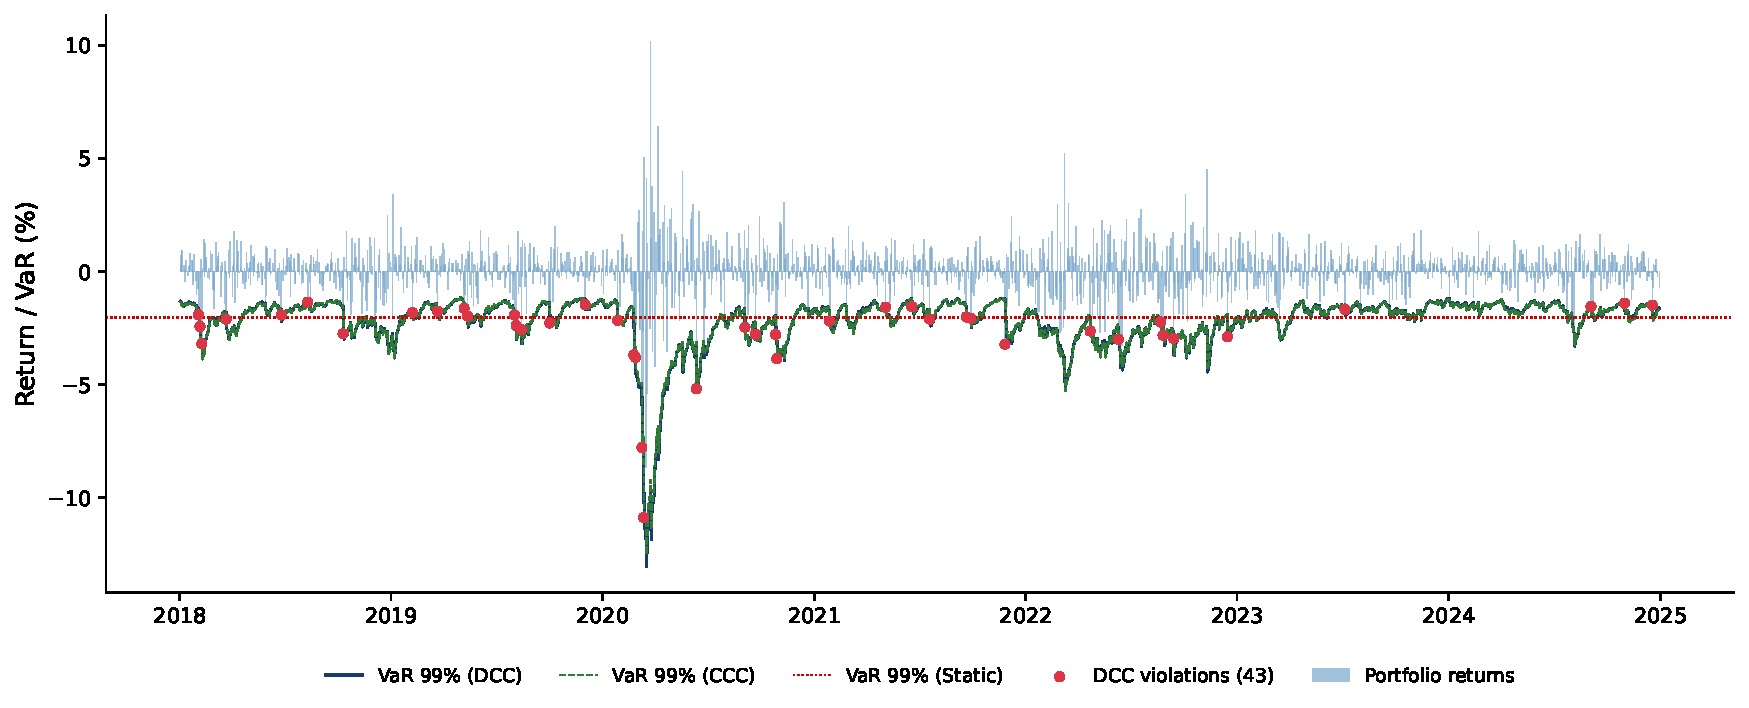
\includegraphics[width=0.92\textwidth, height=0.52\textheight, keepaspectratio]{../../charts/ch5b_var_backtest.pdf}
        \end{center}
    \vspace{-3mm}
    {\scriptsize
    \begin{alertblock}{Interpretare}
        \begin{itemize}\setlength{\itemsep}{0pt}
            \item VaR-ul \textbf{DCC} se ajustează rapid la creșterea corelațiilor din crize --- mai puține violări
            \item VaR-ul \textbf{CCC/static} subestimează riscul în perioade turbulente (corelații presupuse constante)
            \item Violările grupate (\textit{clustered violations}) semnalează eșecul testului de independență Christoffersen
        \end{itemize}
    \end{alertblock}
    }
    \end{cminipage}
    \hfill\quantlet{TSA\_ch5b\_var\_backtest}{https://github.com/QuantLet/TSA/tree/main/TSA\_ch5b/TSA\_ch5b\_var\_backtest}
\end{frame}

\begin{frame}{Studiu de caz 4: VaR și violări pe regimuri de piață}
    \begin{cminipage}{0.95\textwidth}
    \vspace{-3mm}
        \begin{center}
            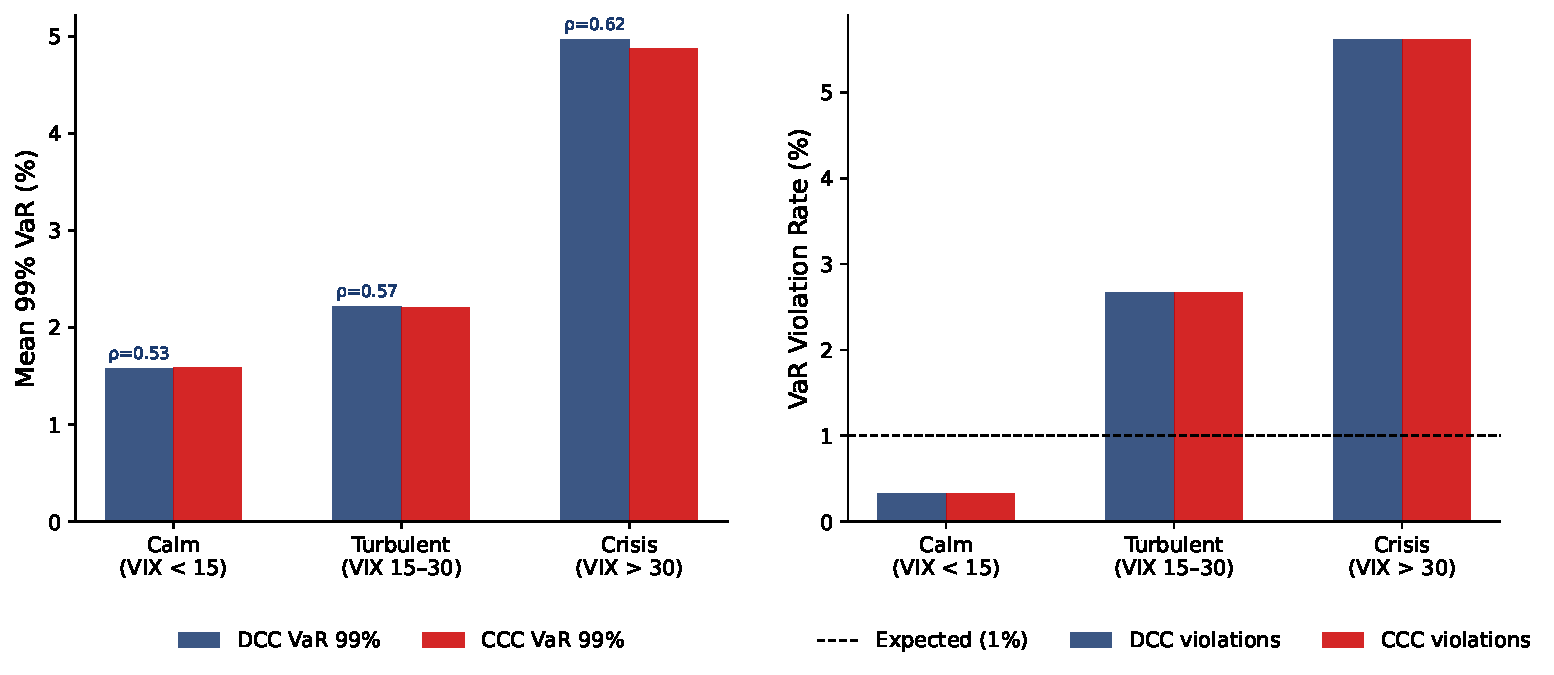
\includegraphics[width=0.92\textwidth, height=0.52\textheight, keepaspectratio]{../../charts/ch5b_var_regime.pdf}
        \end{center}
    \vspace{-3mm}
    {\scriptsize
    \begin{alertblock}{Concluzii}
        \begin{itemize}\setlength{\itemsep}{0pt}
            \item VaR-ul DCC crește \textbf{automat} cu regimul de piață: $\rho_t$ urcă odată cu VIX (\textit{CBOE Volatility Index})
            \item CCC subestimează VaR-ul în criză (VIX $> 30$) cu până la \textbf{30\%} --- violări excesive
            \item \textbf{Lecție}: alege DCC/aDCC pentru active care devin mai corelate în crize (acțiuni, obligațiuni HY)
        \end{itemize}
    \end{alertblock}
    }
    \end{cminipage}
    \hfill\quantlet{TSA\_ch5b\_var\_backtest}{https://github.com/QuantLet/TSA/tree/main/TSA\_ch5b/TSA\_ch5b\_var\_backtest}
\end{frame}

\begin{frame}{Studiu de caz 4: rezultatele testului Christoffersen}
    \begin{cminipage}{0.95\textwidth}
    {\footnotesize
    \begin{block}{Backtesting VaR 99\% (60/40 S\&P 500/DAX, 2004--2024, $T = 5{,}000$)}
        \vspace{0.1cm}
        {\small
        \begin{center}
        \begin{tabular}{l|ccc|ccc}
            \hline
            & \multicolumn{3}{c|}{\textbf{Violări}} & \multicolumn{3}{c}{\textbf{$p$-values Christoffersen}} \\
            \textbf{Model} & Nr. & Rată & Aștept. & UC & Ind & CC \\
            \hline
            DCC    & 52 & 1.04\% & 1\% & 0.82 & 0.45 & 0.67 \\
            CCC    & 71 & 1.42\% & 1\% & 0.02 & 0.03 & 0.01 \\
            Static & 89 & 1.78\% & 1\% & $<$0.01 & $<$0.01 & $<$0.01 \\
            \hline
        \end{tabular}
        \end{center}
        }
    \end{block}
    \begin{alertblock}{Interpretarea rezultatelor}
        \begin{itemize}\setlength{\itemsep}{0pt}
            \item \textbf{DCC}: trece toate cele trei teste --- rata violărilor aproape de 1\% nominal, fără clustering
            \item \textbf{CCC}: eșuează UC ($p = 0.02$) și independența ($p = 0.03$) --- prea multe violări, grupate în crize
            \item \textbf{Static}: eșuează toate testele decisiv --- covarianța constantă este inadecvată pe 20 de ani
            \item Basel III cere $p > 0.05$ pentru aprobarea modelului intern de VaR --- \textbf{doar DCC se califică}
        \end{itemize}
    \end{alertblock}
    }
    \end{cminipage}
\end{frame}

\begin{frame}{Studiu de caz 4: testul Kupiec --- acoperire necondiționată}
    \begin{cminipage}{0.95\textwidth}
    \vspace{-3mm}
    {\scriptsize
    \begin{block}{Setup (Kupiec, 1995)}
        \begin{itemize}\setlength{\itemsep}{0pt}
            \item Indicator de violare: $I_t = \mathbf{1}\{r_{p,t} < -\text{VaR}_t^\alpha\}$, violări: $x = \sum_{t=1}^T I_t$, rata: $\hat{\pi} = x/T$
            \item $H_0$: $\hat{\pi} = \alpha$ (modelul produce acoperirea corectă)
        \end{itemize}
    \end{block}
    \vspace{-2mm}
    \begin{block}{Statistica \textit{Likelihood Ratio}}
        \begin{itemize}\setlength{\itemsep}{0pt}
            \item Sub $H_0$: $x \sim \text{Binomial}(T, \alpha)$. Statistica LR:
            \vspace{-2mm}
            \[
                LR_{UC} = -2\ln\frac{\alpha^x(1-\alpha)^{T-x}}{\hat{\pi}^x(1-\hat{\pi})^{T-x}} \xrightarrow{d} \chi^2(1) \quad \text{sub } H_0
            \]
            \vspace{-3mm}
            \item Se respinge $H_0$ dacă $LR_{UC} > \chi^2_{1,0.05} = 3.84$
        \end{itemize}
    \end{block}
    \vspace{-2mm}
    \begin{alertblock}{Kupiec vs.\ Christoffersen}
        \begin{itemize}\setlength{\itemsep}{0pt}
            \item \textbf{Kupiec} testează doar \textbf{acoperirea} (``sunt prea multe violări?'')
            \item \textbf{Christoffersen} adaugă test de \textbf{independență} (``sunt violările grupate?'') --- mai puternic
            \item \textbf{Combinat} (CC) = UC + Independență: abordarea recomandată
        \end{itemize}
    \end{alertblock}
    }
    \end{cminipage}
\end{frame}

\begin{frame}{Studiu de caz 4: sistemul semafor Basel}
    \begin{cminipage}{0.95\textwidth}
    {\footnotesize
    \begin{block}{Evaluarea regulatorie a modelului VaR (Comitetul Basel, fereastră de 250 zile)}
        \vspace{0.1cm}
        {\small
        \begin{center}
        \begin{tabular}{l|c|c|l}
            \hline
            \textbf{Zonă} & \textbf{Violări} & \textbf{Multipl.\ capital} & \textbf{Acțiune} \\
            \hline
            \textcolor{Forest}{Verde}    & 0--4  & $3.0\times$ & Model acceptat \\
            \textcolor{orange}{Galben}   & 5--9  & $3.4$--$3.85\times$ & Revizie supraveghere \\
            \textcolor{Crimson}{Roșu}    & 10+   & $4.0\times$ & Model respins \\
            \hline
        \end{tabular}
        \end{center}
        }
    \end{block}
    \vspace{-2mm}
    \begin{block}{Cum se clasează modelele noastre? (per fereastră de 250 zile)}
        \vspace{0.1cm}
        {\small
        \begin{center}
        \begin{tabular}{l|c|c|l}
            \hline
            \textbf{Model} & \textbf{Violări medii} & \textbf{Violări max.} & \textbf{Zonă} \\
            \hline
            DCC    & 2.6 & 4  & \textcolor{Forest}{Verde} \\
            CCC    & 3.6 & 7  & \textcolor{orange}{Galben} (criză) \\
            Static & 4.5 & 11 & \textcolor{Crimson}{Roșu} (criză) \\
            \hline
        \end{tabular}
        \end{center}
        }
    \end{block}
    \vspace{-2mm}
    \begin{alertblock}{Implicație}
        \begin{itemize}\setlength{\itemsep}{0pt}
            \item Doar DCC rămâne în zona \textcolor{Forest}{verde} consistent --- băncile cu CCC/static suportă \textbf{cerințe de capital mai mari} în crize
        \end{itemize}
    \end{alertblock}
    }
    \end{cminipage}
\end{frame}

\begin{frame}{Studiu de caz 4: ES vs.\ VaR --- de ce reglementatorii preferă ES}
    \begin{cminipage}{0.95\textwidth}
    {\footnotesize
    \begin{block}{Limitările VaR}
        \begin{itemize}\setlength{\itemsep}{0pt}
            \item VaR răspunde la: \textit{``Care este pierderea maximă cu 99\% încredere?''}
            \item Nu spune \textbf{nimic} despre dimensiunea pierderilor din coada de 1\%
            \item \textbf{Nu este \textit{subadditive}}: $\text{VaR}(A+B)$ poate depăși $\text{VaR}(A) + \text{VaR}(B)$
        \end{itemize}
    \end{block}
    \vspace{-2mm}
    \begin{block}{Expected Shortfall (ES) --- măsură de risc coerentă}
        \begin{itemize}\setlength{\itemsep}{0pt}
            \item ES răspunde la: \textit{``Fiind în coada de 1\%, cât de mare este pierderea medie?''}
            \item $\text{ES}_\alpha = \mathbb{E}[L \,|\, L > \text{VaR}_\alpha]$ --- întotdeauna $\geq$ VaR
            \item \textbf{Subaditivă}: $\text{ES}(A+B) \leq \text{ES}(A) + \text{ES}(B)$ --- diversificarea e recunoscută
        \end{itemize}
    \end{block}
    \vspace{-2mm}
    \begin{alertblock}{Tranziția FRTB (\textit{Fundamental Review of the Trading Book}) (2023+)}
        \begin{itemize}\setlength{\itemsep}{0pt}
            \item \textbf{FRTB} înlocuiește VaR 99\% cu ES 97.5\% ca metrică principală de capital
            \item GARCH multivariat furnizează $\mathbf{H}_t$ necesar pentru calculul VaR și ES
            \item DCC-ES captează \textbf{dependența de coadă} pe care DCC-VaR singur o ratează
        \end{itemize}
    \end{alertblock}
    }
    \end{cminipage}
\end{frame}

\begin{frame}{Studiu de caz 4: \textit{backtesting} ES --- Acerbi \& Szekely (2014)}
    \begin{cminipage}{0.95\textwidth}
    \vspace{-3mm}
    {\scriptsize
    \begin{block}{Problema \textit{backtesting}-ului ES}
        \begin{itemize}\setlength{\itemsep}{0pt}
            \item VaR: numără violări (binar). ES: evaluează \textbf{cât de mari} sunt pierderile când VaR e depășit --- mai dificil
            \item ES nu este \textbf{elicitabil} (Gneiting, 2011) --- nu există scoring simplu doar pentru ES
        \end{itemize}
    \end{block}
    \vspace{-2mm}
    \begin{block}{Statistica de test Acerbi--Szekely}
        \begin{itemize}\setlength{\itemsep}{0pt}
            \item $H_0$: modelul ES este corect specificat. Se definește: $Z_t = \frac{r_{p,t}}{\text{ES}_t^\alpha}\cdot\mathbf{1}\{r_{p,t} < -\text{VaR}_t^\alpha\} + 1$
            \item Sub $H_0$: $\mathbb{E}[Z_t] = 0$. Statistica: $\bar{Z} = \frac{1}{T}\sum_{t=1}^T Z_t$
            \item $\bar{Z} < 0$: ES \textbf{subestimează} pierderile; $\bar{Z} > 0$: ES conservator. Val.\ $p$ prin simulare
        \end{itemize}
    \end{block}
    \vspace{-2mm}
    \begin{alertblock}{Implicații practice}
        \begin{itemize}\setlength{\itemsep}{0pt}
            \item Sub FRTB, băncile fac \textit{backtesting} \textbf{atât} VaR (Christoffersen/Kupiec) cât și ES (Acerbi--Szekely)
            \item DCC cu inovații Student-$t$ trece testele ES; DCC Gaussiană eșuează frecvent
        \end{itemize}
    \end{alertblock}
    }
    \end{cminipage}
\end{frame}

\begin{frame}{Studiu de caz 4: VaR multi-orizont --- scalare și agregare}
    \begin{cminipage}{0.95\textwidth}
    {\footnotesize
    \begin{block}{Scalarea VaR pe orizonturi diferite}
        \begin{itemize}\setlength{\itemsep}{0pt}
            \item \textbf{Regula $\sqrt{T}$}: $\text{VaR}_h = \text{VaR}_1 \times \sqrt{h}$ --- presupune randamente i.i.d.
            \item Cu GARCH: regula \textbf{supraestimează} VaR pe orizont lung (ignoră revenirea la medie a $\sigma_t$)
            \item Abordarea DCC: se simulează $\mathbf{H}_{t+1}, \ldots, \mathbf{H}_{t+h}$ folosind recursia GARCH
        \end{itemize}
    \end{block}
    \vspace{-2mm}
    \begin{exampleblock}{Exemplu: VaR pe 1 zi vs.\ 10 zile (portofoliu 60/40)}
        {\small
        \begin{center}
        \begin{tabular}{l|cc|c}
            \hline
            & \textbf{VaR 1 zi} & \textbf{VaR 10 zile} & \textbf{Factor scalare} \\
            \hline
            Regula $\sqrt{T}$   & 4.16\% & 13.16\% & $\sqrt{10} = 3.16$ \\
            Simulare DCC        & 4.16\% & 11.84\% & 2.85 \\
            \hline
        \end{tabular}
        \end{center}
        }
        \begin{itemize}\setlength{\itemsep}{0pt}
            \item Regula $\sqrt{T}$ supraestimează VaR-ul pe 10 zile cu \textbf{11\%} deoarece ignoră revenirea la medie
        \end{itemize}
    \end{exampleblock}
    \vspace{-2mm}
    \begin{alertblock}{Cerința Basel}
        \begin{itemize}\setlength{\itemsep}{0pt}
            \item Basel cere VaR pe 10 zile pentru capitalul de risc de piață
            \item Simularea DCC în loc de $\sqrt{T}$ poate reduce cerințele de capital cu 8--15\%
        \end{itemize}
    \end{alertblock}
    }
    \end{cminipage}
\end{frame}

\begin{frame}{Studiu de caz 4: sumar --- cifre cheie}
    \begin{cminipage}{0.95\textwidth}
    {\footnotesize
    \begin{block}{Tabel de referință: rezultate backtesting VaR (2004--2024)}
        {\small
        \begin{center}
        \begin{tabular}{l|l}
            \hline
            \textbf{Statistică} & \textbf{Valoare} \\
            \hline
            Rata violărilor DCC (nominal 1\%) & 1.04\% \\
            Rata violărilor CCC              & 1.42\% ($+$42\% exces) \\
            Rata violărilor static           & 1.78\% ($+$78\% exces) \\
            DCC: Christoffersen CC $p$-value & 0.67 (trece) \\
            CCC: Christoffersen CC $p$-value & 0.01 (eșuează) \\
            Subestimarea VaR de criză CCC    & până la 30\% \\
            Zona Basel (DCC)                 & \textcolor{Forest}{Verde} mereu \\
            Zona Basel (Static, criză)       & \textcolor{Crimson}{Roșu} \\
            Beneficiul diversificării ($\rho = 0.5$) & 15\% reducere VaR \\
            Beneficiul diversificării ($\rho = 0.95$) & 2\% reducere VaR \\
            \hline
        \end{tabular}
        \end{center}
        }
    \end{block}
    \vspace{-2mm}
    \begin{alertblock}{Concluzie}
        \begin{itemize}\setlength{\itemsep}{0pt}
            \item DCC este singurul model care trece consistent backtesting-ul regulatoriu pe toate regimurile de piață
            \item Costul utilizării CCC sau static este atât regulatoriu (capital mai mare) cât și economic (subestimarea riscului de coadă)
        \end{itemize}
    \end{alertblock}
    }
    \end{cminipage}
\end{frame}

%--- Studiu de caz 5: Monitorizarea riscului sistemic ---
\begin{frame}{Studiu de caz 5: ce este riscul sistemic?}
    \vspace{-2mm}
    {\scriptsize\textit{Obiectiv didactic: legătura dintre corelațiile DCC și măsurile de risc sistemic ($\Delta$CoVaR, MES, SRISK) și identificarea G-SIB.}}\vspace{1mm}
    \begin{cminipage}{0.95\textwidth}
    {\scriptsize
    \begin{block}{Definiție}
        \begin{itemize}\setlength{\itemsep}{0pt}
            \item \textbf{Riscul sistemic}: dificultățile unei instituții declanșează eșecuri în cascadă în întregul sistem financiar
        \end{itemize}
    \end{block}
    \vspace{-2mm}
    \begin{block}{Caracteristici cheie}
        \begin{itemize}\setlength{\itemsep}{0pt}
            \item \textbf{Too Big / Too Connected to Fail}: eșecul destabilizează sistemul prin contagiune
            \item \textbf{Explozie de corelații}: în crize, corelațiile cresc $\Rightarrow$ diversificarea dispare
            \item \textbf{Non-liniaritate}: riscul sistemic apare din \textbf{interacțiuni}, nu din suma riscurilor individuale
        \end{itemize}
    \end{block}
    \vspace{-2mm}
    \begin{alertblock}{De ce MGARCH?}
        \begin{itemize}\setlength{\itemsep}{0pt}
            \item Riscul sistemic = \textbf{comportament comun de coadă} al mai multor instituții
            \item DCC-GARCH furnizează $\mathbf{H}_t$ variabil în timp, necesar pentru calculul măsurilor condiționale de risc
            \item Corelațiile statice ratează amplificarea din criză care definește evenimentele sistemice
        \end{itemize}
    \end{alertblock}
    }
    \end{cminipage}
\end{frame}

\begin{frame}{Studiu de caz 5: monitorizarea riscului sistemic}
    \begin{cminipage}{0.95\textwidth}
    {\footnotesize
    \begin{block}{Indicatori de risc sistemic bazați pe MGARCH}
        \begin{itemize}\setlength{\itemsep}{0pt}
            \item \textbf{CoVaR} (\textit{Conditional Value at Risk}; Adrian \& Brunnermeier, 2016): VaR-ul sistemului condițional de stresul unei instituții
            \[
                \Delta\text{CoVaR}_{i,t} = \text{VaR}_{t}^{\text{sistem} | i \text{ în stres}} - \text{VaR}_{t}^{\text{sistem} | i \text{ normal}}
            \]
            \item \textbf{Indicele de conectivitate DCC}: $C_t = \frac{2}{N(N-1)}\sum_{i<j}|\rho_{ij,t}|$ --- media corelațiilor
            \item Când $C_t \rightarrow 1$ simultan $\Rightarrow$ diversificarea dispare $\Rightarrow$ \textbf{semnal de criză}
        \end{itemize}
    \end{block}
    \begin{alertblock}{Cerințe reglementare}
        \begin{itemize}\setlength{\itemsep}{0pt}
            \item \textbf{Basel III/IV}: băncile trebuie să raporteze VaR pe orizonturi multiple cu corelații dinamice
            \item \textbf{FRTB} (\textit{Fundamental Review of the Trading Book}): înlocuiește VaR cu ES, necesită GARCH multivariat
            \item \textbf{DCC-GARCH} furnizează matricea $\mathbf{H}_t$ necesară pentru calculul CoVaR și stress testing
        \end{itemize}
    \end{alertblock}
    }
    \end{cminipage}
\end{frame}

\begin{frame}{Studiu de caz 5: indicele de conectivitate DCC în timp}
    \begin{cminipage}{0.95\textwidth}
    \vspace{-3mm}
        \begin{center}
            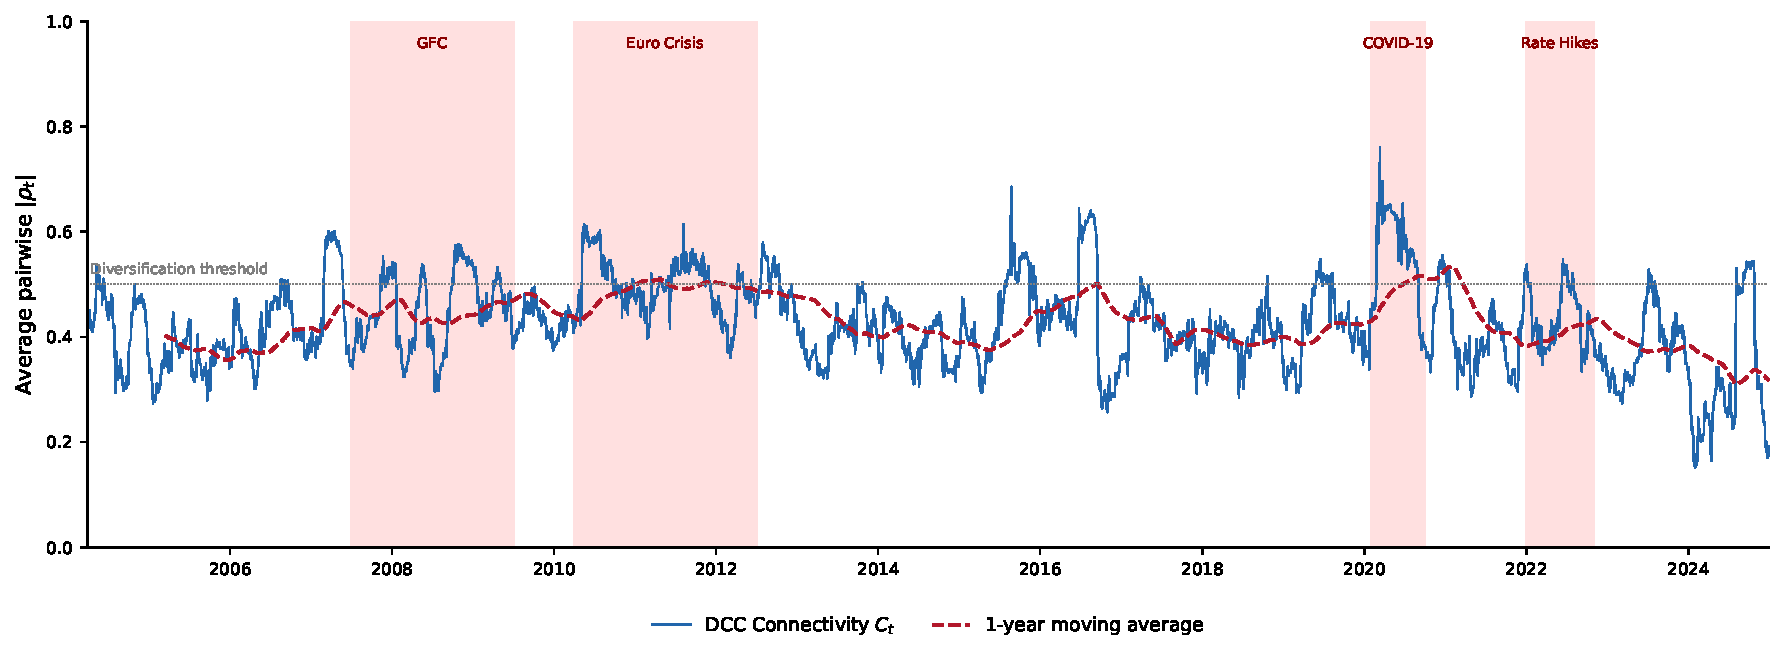
\includegraphics[width=0.92\textwidth, height=0.52\textheight, keepaspectratio]{../../charts/ch5b_dcc_connectivity.pdf}
        \end{center}
    \vspace{-3mm}
    {\scriptsize
    \begin{alertblock}{Interpretare}
        \begin{itemize}\setlength{\itemsep}{0pt}
            \item $C_t$ sare de la $\sim$0.45 (normal) la $>$0.85 în GFC și COVID --- \textbf{diversificarea dispare}
            \item Creșterea conectivității \textbf{precede} vârful pierderilor cu 2--3 săptămâni --- semnal de avertizare
            \item Normalizarea post-criză durează 6--12 luni, creând o fereastră de \textbf{\textit{false security}}
            \item Când $C_t > 0.5$: beneficiile diversificării sunt \textbf{semnificativ reduse}
        \end{itemize}
    \end{alertblock}
    }
    \end{cminipage}
\end{frame}

\begin{frame}{Studiu de caz 5: exemplu numeric --- $\Delta$CoVaR}
    \begin{cminipage}{0.95\textwidth}
    \vspace{-3mm}
    {\scriptsize
    \begin{exampleblock}{4 bănci: $\sigma_i = 2.5\%$, $\rho_{i,\text{sys}} = 0.72$, $\sigma_{\text{sys}} = 1.8\%$}
        \begin{itemize}\setlength{\itemsep}{0pt}
            \item Normal: $\text{VaR}^{\text{sys}} = 2.326 \times 1.8\% = 4.19\%$. Sub stres ($\kappa \approx 2.5$):
            \vspace{-2mm}
            \[
                \sigma_{\text{sys}|i} = \sigma_{\text{sys}}\sqrt{1 + \rho_{i,\text{sys}}^2(\kappa - 1)} = 1.8\% \times 1.33 = 2.39\%
            \]
            \vspace{-4mm}
        \end{itemize}
    \end{exampleblock}
    \vspace{-2mm}
    \begin{block}{Rezultat}
        \begin{itemize}\setlength{\itemsep}{0pt}
            \item $\text{CoVaR}^{\text{sys}|i} = 2.326 \times 2.39\% = 5.56\%$
            \item $\Delta\text{CoVaR}_i = 5.56\% - 4.19\% = \textcolor{Crimson}{\mathbf{1.37\%}}$ --- stresul băncii $i$ adaugă \textbf{33\%} la riscul sistemic
        \end{itemize}
    \end{block}
    \vspace{-2mm}
    \begin{alertblock}{Implicație regulatorie}
        \begin{itemize}\setlength{\itemsep}{0pt}
            \item Băncile cu $\Delta$CoVaR ridicat suportă \textbf{suplimente de capital} (buffere G-SIB --- \textit{Global Systemically Important Bank})
            \item DCC este esențial: cu CCC ($\rho$ fix), $\Delta$CoVaR ratează amplificarea din crize
            \item În GFC, $\Delta$CoVaR pentru top-5 bănci americane a depășit \textbf{3\%} --- de trei ori nivelul normal
        \end{itemize}
    \end{alertblock}
    }
    \end{cminipage}
\end{frame}

\begin{frame}{Studiu de caz 5: MES --- Marginal Expected Shortfall}
    \begin{cminipage}{0.95\textwidth}
    \vspace{-2mm}
    {\scriptsize
    \begin{block}{Definiție (Acharya et al., 2017)}
        \begin{itemize}\setlength{\itemsep}{0pt}
            \item \textbf{MES} (\textit{Marginal Expected Shortfall}): pierderea așteptată a instituției $i$ când sistemul se află în coadă:
            $\text{MES}_{i,t} = \mathbb{E}\left[r_{i,t} \;\middle|\; r_{\text{sys},t} < \text{VaR}_{\text{sys},t}^\alpha\right]$
            \item DCC: $\mathbb{E}[r_i | r_{\text{sys}}] = \rho_{i,\text{sys},t} \cdot \frac{\sigma_{i,t}}{\sigma_{\text{sys},t}} \cdot r_{\text{sys}}$
        \end{itemize}
    \end{block}
    \vspace{-2mm}
    \begin{exampleblock}{Exemplu numeric}
        \begin{itemize}\setlength{\itemsep}{0pt}
            \item Banca $i$: $\sigma_i = 2.5\%$, $\rho_{i,\text{sys}} = 0.72$; Sistem: $\sigma_{\text{sys}} = 1.8\%$
            \item Crash sistemic de 2$\sigma$ ($r_{\text{sys}} = -3.6\%$):
            $\text{MES}_i = 0.72 \times \frac{2.5}{1.8} \times 3.6\% = \textcolor{Crimson}{\mathbf{3.60\%}}$
        \end{itemize}
    \end{exampleblock}
    \vspace{-2mm}
    \begin{alertblock}{MES vs.\ CoVaR}
        \begin{itemize}\setlength{\itemsep}{0pt}
            \item MES măsoară contribuția \textbf{băncii la sistem} (expunere)
            \item CoVaR măsoară impactul \textbf{sistemului asupra băncii} (contagiune)
            \item Ambele necesită DCC-GARCH
        \end{itemize}
    \end{alertblock}
    }
    \end{cminipage}
\end{frame}

\begin{frame}{Studiu de caz 5: SRISK --- deficit de capital sub stres}
    \begin{cminipage}{0.95\textwidth}
    \vspace{-2mm}
    {\scriptsize
    \begin{block}{Definiție (Brownlees \& Engle, 2017)}
        \begin{itemize}\setlength{\itemsep}{0pt}
            \item \textbf{SRISK} (\textit{Systemic Risk}): deficitul de capital așteptat în cazul unei crize sistemice
            \vspace{-1mm}
            \[
                \text{SRISK}_{i,t} = k \cdot D_{i,t} - (1-k) \cdot W_{i,t} \cdot (1 - \text{LRMES}_{i,t})
            \]
            \vspace{-4mm}
            \item $k = 8\%$ (raport prudențial), $D$: datorie, $W$: capitalizare bursieră, \textbf{LRMES} (\textit{Long-Run Marginal Expected Shortfall}): pierderea capitalului propriu într-o scădere de 40\% a pieței (6 luni)
        \end{itemize}
    \end{block}
    \vspace{-2mm}
    \begin{block}{Rolul DCC-GARCH în SRISK}
        \begin{itemize}\setlength{\itemsep}{0pt}
            \item DCC furnizează $\rho_{i,\text{sys},t}$ și $\sigma_{i,t}$ $\Rightarrow$ MES $\Rightarrow$ LRMES (simulare DCC pe 6 luni)
            \item SRISK se actualizează \textbf{zilnic} pe măsură ce capitalizarea și corelațiile DCC se schimbă
        \end{itemize}
    \end{block}
    \vspace{-2mm}
    \begin{alertblock}{Aplicație}
        \begin{itemize}\setlength{\itemsep}{0pt}
            \item NYU Stern V-Lab publică \textbf{clasamente SRISK zilnice} pentru peste 1200 firme financiare globale, bazate pe DCC-GARCH: \texttt{vlab.stern.nyu.edu}
        \end{itemize}
    \end{alertblock}
    }
    \end{cminipage}
\end{frame}

\begin{frame}{Studiu de caz 5: identificarea G-SIB și suplimente de capital}
    \begin{cminipage}{0.95\textwidth}
    \vspace{-4mm}
    {\scriptsize
    \begin{block}{Cum identifică reglementatorii băncile de importanță sistemică}
        \begin{itemize}\setlength{\itemsep}{0pt}
            \item \textbf{FSB} (\textit{Financial Stability Board})\textbf{/Basel}: scor G-SIB = dimensiune + interconectare + substituibilitate + complexitate + activitate transfrontalieră
            \item \textbf{Măsuri bazate pe piață}: $\Delta$CoVaR, MES, SRISK complementează scorurile regulatorii
        \end{itemize}
    \end{block}
    \vspace{-2mm}
    \begin{block}{Suplimentele de capital G-SIB (2024)}
        {\small
        \begin{center}
        \begin{tabular}{l|c|l}
            \hline
            \textbf{Bucket} & \textbf{Supliment} & \textbf{Exemple bănci} \\
            \hline
            5 (cel mai înalt)   & 3.5\% & JPMorgan \\
            4                   & 2.5\% & HSBC, Citi \\
            3                   & 2.0\% & BNP Paribas, Goldman Sachs \\
            2                   & 1.5\% & Deutsche Bank, UBS \\
            1                   & 1.0\% & Santander, Standard Chartered \\
            \hline
        \end{tabular}
        \end{center}
        }
    \end{block}
    \vspace{-2mm}
    \begin{alertblock}{Punct cheie}
        \begin{itemize}\setlength{\itemsep}{0pt}
            \item Conectivitate DCC mai mare $\Rightarrow$ importanță sistemică mai mare $\Rightarrow$ buffere de capital mai mari $\Rightarrow$ ROE (\textit{Return on Equity}) mai mic
            \item Măsurarea precisă a $\rho_{ij,t}$ are \textbf{consecințe financiare directe}
        \end{itemize}
    \end{alertblock}
    }
    \end{cminipage}
\end{frame}

\begin{frame}{Studiu de caz 5: rețele de contagiune --- vizualizarea interconectivității}
    \begin{cminipage}{0.95\textwidth}
    {\footnotesize
    \begin{block}{De la corelații pereche la topologia rețelei}
        \begin{itemize}\setlength{\itemsep}{0pt}
            \item DCC produce $N(N-1)/2$ corelații pereche $\rho_{ij,t}$ la fiecare moment $t$
            \item Se construiește un \textbf{graf ponderat}: noduri = instituții, \textit{edge weight} = $|\rho_{ij,t}|$
            \item Metrici de rețea: \textbf{centralitate de grad}, \textbf{betweenness} (rol de punte), \textbf{centralitate de vector propriu}
        \end{itemize}
    \end{block}
    \vspace{-2mm}
    \begin{block}{Structura rețelei: criză vs.\ normal}
        {\small
        \begin{center}
        \begin{tabular}{l|cc}
            \hline
            \textbf{Proprietatea rețelei} & \textbf{Normal} & \textbf{Criză} \\
            \hline
            Media $|\rho_{ij}|$          & 0.45 & 0.85 \\
            Densitatea rețelei           & 0.35 & 0.90 \\
            Coeficient de clustering     & 0.52 & 0.88 \\
            Nodul cel mai central        & JPMorgan & JPMorgan \\
            \hline
        \end{tabular}
        \end{center}
        }
    \end{block}
    \vspace{-2mm}
    \begin{alertblock}{Concluzie}
        \begin{itemize}\setlength{\itemsep}{0pt}
            \item În perioade normale, rețeaua este \textbf{\textit{sparse}} --- șocurile rămân locale
            \item În crize, devine \textbf{densă și complet conectată} --- diversificarea devine imposibilă
        \end{itemize}
    \end{alertblock}
    }
    \end{cminipage}
\end{frame}

\begin{frame}{Studiu de caz 5: DCC pentru testarea de stres regulatorie}
    \begin{cminipage}{0.95\textwidth}
    \vspace{-2mm}
    {\footnotesize
    \begin{block}{Cum folosesc băncile centrale DCC-GARCH}
        \begin{itemize}\setlength{\itemsep}{1pt}
            \item \textbf{Testele de stres ECB (\textit{European Central Bank})/Fed}: simularea randamentelor activelor în scenarii adverse
            \item DCC furnizează \textbf{structura corelațiilor} pentru scenariu: ``dacă acțiunile scad cu 40\%, ce se întâmplă cu spread-urile de credit?''
            \item Cheie: folosiți parametri DCC \textbf{calibrați pe criză}, nu medii pe întreg eșantionul
        \end{itemize}
    \end{block}
    \vspace{-2mm}
    \begin{block}{Fluxul de lucru pentru testarea de stres}
        \begin{enumerate}\setlength{\itemsep}{0pt}
            \item Estimați DCC-GARCH pe 10+ ani de date
            \item Extrageți parametrii $\alpha, \beta$ din subperioada de criză (ex.\ GFC)
            \item Simulați 10.000 de traiectorii $\mathbf{H}_{t+1}, \ldots, \mathbf{H}_{t+h}$ sub parametri de stres
            \item Calculați distribuția pierderilor portofoliului $\Rightarrow$ VaR, ES, SRISK sub stres
        \end{enumerate}
    \end{block}
    \vspace{-2mm}
    \begin{alertblock}{De ce nu simulare istorică?}
        \begin{itemize}\setlength{\itemsep}{0pt}
            \item Simularea istorică folosește randamente \textbf{trecute} direct --- dar nicio criză nu seamănă cu alta
            \item Testarea de stres DCC generează scenarii \textbf{noi} de criză consistente cu dinamica estimată a corelațiilor
        \end{itemize}
    \end{alertblock}
    }
    \end{cminipage}
\end{frame}

\begin{frame}{Studiu de caz 5: sumar --- setul de instrumente pentru risc sistemic}
    \begin{cminipage}{0.95\textwidth}
    {\footnotesize
    \begin{block}{Măsuri de risc sistemic bazate pe DCC}
        \vspace{0.1cm}
        {\small
        \begin{center}
        \begin{tabular}{l|l|l}
            \hline
            \textbf{Măsură} & \textbf{Ce captează} & \textbf{Input cheie din DCC} \\
            \hline
            $C_t$ (conectivitate) & Corelație la nivel de sistem & media $|\rho_{ij,t}|$ \\
            $\Delta$CoVaR         & Impactul unei bănci asupra VaR sistem & $\rho_{i,\text{sys},t}$, $\sigma_{i,t}$ \\
            MES                   & Pierderea băncii la crash sistemic & $\rho_{i,\text{sys},t}$, $\sigma_{i,t}$ \\
            SRISK                 & Deficit de capital sub stres & LRMES din simulare DCC \\
            Spillover DY          & Transmisia volatilității între piețe & VAR pe reziduuri DCC \\
            \hline
        \end{tabular}
        \end{center}
        }
    \end{block}
    \begin{alertblock}{Concluzii cheie}
        \begin{itemize}\setlength{\itemsep}{0pt}
            \item DCC-GARCH este \textbf{coloana vertebrală} a măsurării moderne a riscului sistemic
            \item Toți indicatorii majori ($\Delta$CoVaR, MES, SRISK) necesită $\rho_{ij,t}$ variabil în timp
            \item Indicele de conectivitate $C_t > 0.7$ este un \textbf{semnal de avertizare} fiabil pentru crize sistemice
            \item Aplicații regulatorii: identificarea G-SIB, suplimente de capital, testare de stres
        \end{itemize}
    \end{alertblock}
    }
    \end{cminipage}
\end{frame}

%=============================================================================
% SECȚIUNEA 11: DINCOLO DE MGARCH --- ABORDĂRI MODERNE
%=============================================================================
\section{Dincolo de MGARCH: abordări moderne}

\begin{frame}{\textit{Realized Covariance} și HAR-DRD}
    \begin{cminipage}{0.95\textwidth}
    \vspace{-3mm}
    {\scriptsize
    \begin{block}{De la parametric la nonparametric: \textit{Realized Covariance}}
        \begin{itemize}\setlength{\itemsep}{0pt}
            \item În loc de a \textit{modela} $\mathbf{H}_t$, o \textbf{măsurăm} direct din date intraday: $\mathbf{RC}_t = \sum_{k=1}^{M} \mathbf{r}_{t,k}\mathbf{r}_{t,k}'$ ($M$ = nr.\ intervale, ex.\ 5 min)
            \item \textbf{Fără model}: nu sunt necesare presupuneri GARCH --- datele ``vorbesc de la sine''
            \item Necesită \textbf{date de înaltă frecvență} --- indisponibile pentru toate activele (obligațiuni, derivate OTC)
        \end{itemize}
    \end{block}
    \vspace{-2mm}
    \begin{block}{Modelul HAR-DRD (Shephard \& Sheppard, 2010; Oh \& Patton, 2016)}
        \begin{itemize}\setlength{\itemsep}{0pt}
            \item Descompunere: $\mathbf{RC}_t = \mathbf{D}_t^{RC}\mathbf{R}_t^{RC}\mathbf{D}_t^{RC}$ (analog DCC dar cu măsuri realizate)
            \item Volatilități realizate cu dinamici HAR: $d_{i,t+1} = c + \beta_d d_{i,t} + \beta_w \bar{d}_{i,t}^{(w)} + \beta_m \bar{d}_{i,t}^{(m)} + \varepsilon_{t+1}$
            \item $\bar{d}^{(w)}$, $\bar{d}^{(m)}$ = medii săptămânale, lunare --- captează traderi eterogeni
        \end{itemize}
    \end{block}
    \vspace{-2mm}
    \begin{alertblock}{Când se utilizează}
        \begin{itemize}\setlength{\itemsep}{0pt}
            \item \textbf{De preferat} când datele intraday sunt disponibile --- domină MGARCH în previziuni (Lunde et al., 2016)
        \end{itemize}
    \end{alertblock}
    }
    \end{cminipage}
\end{frame}

\begin{frame}{DCC-MIDAS: separarea dinamicilor pe termen scurt și lung}
    \begin{cminipage}{0.95\textwidth}
    \vspace{-3mm}
    {\scriptsize
    \begin{block}{Motivație}
        \begin{itemize}\setlength{\itemsep}{0pt}
            \item DCC standard are \textbf{o singură scală temporală} --- nu distinge fluctuațiile zilnice de tendințele seculare
            \item Corelațiile au componentă \textbf{pe termen lung} (factori macro) și \textbf{pe termen scurt} (știri)
        \end{itemize}
    \end{block}
    \vspace{-2mm}
    \begin{block}{DCC-MIDAS (Colacito, Engle \& Ghysels, 2011)}
        \begin{itemize}\setlength{\itemsep}{0pt}
            \item $\bar{Q}_t$ variabil în timp: $\bar{q}_{ij,t} = \sum_{k=1}^{K} \varphi_k(\omega_1, \omega_2)\, c_{ij,t-k}$, \; $c_{ij,t} = \frac{1}{N_v}\sum_{n=1}^{N_v} z_{i,t_n}z_{j,t_n}$
            \item $\varphi_k$ = schema de ponderare Beta (MIDAS --- \textit{Mixed Data Sampling})
            \item Dinamici DCC pe termen scurt în jurul lui $\bar{q}_{ij,t}$ care se mișcă lent
        \end{itemize}
    \end{block}
    \vspace{-2mm}
    \begin{alertblock}{Avantaj față de DCC standard}
        \begin{itemize}\setlength{\itemsep}{0pt}
            \item Captează \textbf{\textit{structural breaks}} natural --- $\bar{q}_{ij,t}$ se adaptează la noile regimuri
            \item Previziuni mai bune pe orizont lung (1 lună+) --- DCC standard revine prea rapid la $\bar{Q}$
        \end{itemize}
    \end{alertblock}
    }
    \end{cminipage}
\end{frame}

\begin{frame}{\textit{Machine Learning} pentru previziunea covarianței}
    \begin{cminipage}{0.95\textwidth}
    \vspace{-2mm}
    {\scriptsize
    \begin{block}{De ce ML? Limitări ale MGARCH parametric}
        \begin{itemize}\setlength{\itemsep}{0pt}
            \item MGARCH presupune o \textbf{formă funcțională fixă} --- ML poate învăța dinamici neliniare direct din date
            \item Previziunea covarianței în dimensiune mare ($N > 100$) este intractabilă pentru MGARCH clasic --- ML scalează mai bine
        \end{itemize}
    \end{block}
    \vspace{-1mm}
    \begin{block}{Abordări (Bucci, 2020; De Nard et al., 2021; Zhang et al., 2023)}
        \begin{itemize}\setlength{\itemsep}{0pt}
            \item \textbf{Rețele LSTM / GRU}: tratează $\text{vech}(\mathbf{H}_t)$ ca serie temporală multivariată --- captează dependențe de lungă durată
            \item \textbf{Modele \textit{Transformer}}: mecanismul de atenție identifică care corelații trecute sunt cele mai relevante
            \item \textbf{\textit{Graph Neural Networks}}: modelează relațiile între active ca graf --- natural pentru analiză de contagiune
            \item \textbf{Hibrid DCC-ML}: DCC ca bază, ML corectează reziduurile (Gu, Kelly \& Xiu, 2020)
        \end{itemize}
    \end{block}
    \vspace{-1mm}
    \begin{alertblock}{Status actual}
        \begin{itemize}\setlength{\itemsep}{0pt}
            \item Abordările ML sunt promițătoare pentru \textbf{$N$ mare} și \textbf{regimuri neliniare}, dar le lipsește interpretabilitatea
            \item \textbf{Fără consens} că ML bate consistent DCC pentru $N$ moderat ($< 50$)
            \item Abordările hibride (DCC + corecții ML) sunt cea mai promițătoare direcție curentă
        \end{itemize}
    \end{alertblock}
    }
    \end{cminipage}
\end{frame}

\begin{frame}{\textit{Conformal Prediction} pentru calibrarea covarianței}
    \begin{cminipage}{0.95\textwidth}
    \vspace{-1mm}
    {\footnotesize
    \begin{block}{Problema calibrării}
        \begin{itemize}\setlength{\itemsep}{0pt}
            \item VaR-ul MGARCH presupune o \textbf{distribuție specifică} (Gaussiană, Student-$t$) --- specificarea greșită duce la acoperire slabă
            \item Chiar cu covarianța corectă, \textbf{presupunerea distribuțională} poate eșua în cozi
        \end{itemize}
    \end{block}
    \begin{block}{\textit{Conformal Prediction} (Vovk et al., 2005; Gibbs \& Cand\`es, 2021)}
        \begin{itemize}\setlength{\itemsep}{0pt}
            \item Garanție de acoperire \textbf{fără distribuție}: produce mulțimi de predicție cu acoperire exactă $1-\alpha$
            \item Aplicată la VaR: ajustează cuantila folosind reziduurile trecute, nu presupuneri parametrice
            \item \textbf{\textit{Adaptive Conformal Inference}} (ACI): ajustează acoperirea în timp real --- se strânge în calm, se lărgește în criză
        \end{itemize}
    \end{block}
    \begin{alertblock}{Integrare cu MGARCH}
        \begin{itemize}\setlength{\itemsep}{0pt}
            \item Se folosește DCC-GARCH pentru \textbf{previziunea punctuală} a lui $\mathbf{H}_t$, apoi se conformalizează limitele VaR/ES
            \item Obține \textbf{acoperire garantată} chiar când DCC este specificat greșit --- ce e mai bun din ambele lumi
            \item Domeniu activ de cercetare --- Nolde \& Ziegel (2017), Barber et al.\ (2023)
        \end{itemize}
    \end{alertblock}
    }
    \end{cminipage}
\end{frame}

%=============================================================================
% SECȚIUNEA 12: REZUMAT ȘI TEST
%=============================================================================
\section{Rezumat}

\begin{frame}{Rezumat: concluzii cheie}
    \begin{cminipage}{0.95\textwidth}
    {\footnotesize
    \begin{block}{Ce am învățat}
        \begin{enumerate}\setlength{\itemsep}{2pt}
            \item GARCH multivariat modelează \textbf{matricea de covarianță variabilă în timp} $\mathbf{H}_t$
            \item Provocarea principală: \textbf{curse of dimensionality} --- $N(N+1)/2$ elemente unice
            \item \textbf{VEC/BEKK}: parametrizare directă --- flexibil dar limitat la $N$ mic
            \item \textbf{CCC}: corelații constante --- \textit{parsimonious} dar nerealist
            \item \textbf{DCC}: corelații dinamice cu doar 2 parametri suplimentari --- modelul de referință
            \item \textbf{aDCC}: adaugă asimetrie în corelații (efect de levier)
            \item \textbf{Factor/GO-GARCH}: pentru $N$ mare prin reducerea dimensionalității
            \item Estimarea în două etape face DCC/CCC fezabile pentru sute de active
        \end{enumerate}
    \end{block}
    \begin{alertblock}{Mesajul central}
        \begin{itemize}\setlength{\itemsep}{0pt}
            \item Corelațiile \textbf{nu sunt constante} --- ignorarea lor duce la \textbf{subestimarea riscului}
            \item Deciziile sub-optime de hedging și alocare rezultă din covarianțe statice
        \end{itemize}
    \end{alertblock}
    }
    \end{cminipage}
\end{frame}

\begin{frame}{\textit{Pipeline} practic: pregătirea datelor}
    \begin{cminipage}{0.95\textwidth}
    {\scriptsize
    \begin{block}{Pasul 1: colectarea și curățarea datelor}
        \begin{itemize}\setlength{\itemsep}{0pt}
            \item Se utilizează \textbf{log-randamente} $\times 100$ (procente) --- stabilizează optimizarea
            \item Se aliniază toate seriile pe \textbf{date comune de tranzacționare} (se elimină sărbătorile, zilele fără suprapunere)
            \item Se gestionează \textbf{tranzacționarea nesincronă}: pentru active din fusuri orare diferite, se folosesc randamente \textit{open-to-open} sau corecția Scholes--Williams
        \end{itemize}
    \end{block}
    \vspace{-1mm}
    \begin{block}{Pasul 2: analiză preliminară}
        \begin{itemize}\setlength{\itemsep}{0pt}
            \item \textbf{Corelații pe fereastră mobilă} (60 zile, 252 zile) --- verificare vizuală a variației în timp
            \item Test \textbf{corelație constantă}: Engle--Sheppard (2001) sau LM Tse (2000)
            \item Test \textbf{efecte ARCH}: LM Engle (1982) pe randamentele pătrate
            \item Verificare \textbf{\textit{structural breaks}}: grafic corelații vs.\ VIX
        \end{itemize}
    \end{block}
    \vspace{-1mm}
    \begin{alertblock}{Punct de decizie}
        \begin{itemize}\setlength{\itemsep}{0pt}
            \item CCC \textbf{nu este respins}: se folosește CCC (mai simplu, mai puțini parametri)
            \item CCC \textbf{este respins}: se trece la DCC/aDCC
        \end{itemize}
    \end{alertblock}
    }
    \end{cminipage}
\end{frame}

\begin{frame}{\textit{Pipeline} practic: estimare și selecția modelului}
    \begin{cminipage}{0.95\textwidth}
    \vspace{-2mm}
    {\scriptsize
    \begin{block}{Pasul 3: specificarea GARCH univariat}
        \begin{itemize}\setlength{\itemsep}{0pt}
            \item Se estimează \textbf{GARCH(1,1)} sau \textbf{GJR-GARCH(1,1)} pentru fiecare serie individual
            \item Se utilizează AIC/BIC pentru a selecta cea mai bună specificare univariată \textbf{per activ}
            \item Se verifică: $\alpha + \beta < 1$ (stationaritate), reziduurile trec testul Ljung--Box
        \end{itemize}
    \end{block}
    \vspace{-1mm}
    \begin{block}{Pasul 4: estimarea modelului multivariat}
        \begin{itemize}\setlength{\itemsep}{0pt}
            \item \textbf{$N \leq 5$}: se estimează DCC, aDCC și Diagonal BEKK; comparare cu AIC/BIC
            \item \textbf{$5 < N \leq 50$}: se estimează doar DCC și aDCC (BEKK infezabil)
            \item \textbf{$N > 50$}: DCC cu \textit{composite likelihood}, sau Factor GARCH
            \item Se inițializează din \textbf{EWMA} ($\lambda = 0.94$) sau matricea de corelație din eșantion
        \end{itemize}
    \end{block}
    \vspace{-1mm}
    \begin{block}{Pasul 5: diagnostice}
        \begin{itemize}\setlength{\itemsep}{0pt}
            \item Se verifică reziduurile standardizate $\hat{z}_{it}$: fără corelație serială (Ljung--Box), fără efecte ARCH reziduale
            \item Se verifică produsele încrucișate $\hat{z}_{it}\hat{z}_{jt}$: fără corelație încrucișată reziduală (Hosking, 1980)
            \item Se compară CCC vs.\ DCC prin testul LR: $LR = 2(\mathcal{L}_{DCC} - \mathcal{L}_{CCC}) \sim \chi^2(2)$
        \end{itemize}
    \end{block}
    }
    \end{cminipage}
\end{frame}

\begin{frame}{\textit{Pipeline} practic: validare și aplicare}
    \begin{cminipage}{0.95\textwidth}
    \vspace{-2mm}
    {\scriptsize
    \begin{block}{Pasul 6: validare \textit{out-of-sample}}
        \begin{itemize}\setlength{\itemsep}{0pt}
            \item Date: \textbf{70\% antrenare}, \textbf{30\% testare} (sau fereastră expandabilă)
            \item Previzionare $\hat{\mathbf{H}}_{t+1}$ cu un pas înainte, calcul VaR/ES portofoliu
            \item \textit{Backtesting}: Kupiec (UC), Christoffersen (CC), Acerbi--Szekely (ES)
            \item Comparare modele: \textbf{\textit{Model Confidence Sets}} sau Diebold--Mariano pe funcții de pierdere
        \end{itemize}
    \end{block}
    \vspace{-1mm}
    \begin{block}{Pasul 7: aplicare}
        \begin{itemize}\setlength{\itemsep}{0pt}
            \item \textbf{Optimizare portofoliu}: $\mathbf{w}_t = \mathbf{H}_t^{-1}\mathbf{1} / (\mathbf{1}'\mathbf{H}_t^{-1}\mathbf{1})$ (varianță minimă)
            \item \textbf{\textit{Hedging}}: $h_t^* = \sigma_{12,t}/\sigma_{22,t}$ (raport dinamic)
            \item \textbf{Raportare risc}: VaR/ES zilnic cu corelații variabile în timp
            \item \textbf{Re-estimare} la fiecare 1--2 ani sau după \textit{structural breaks}
        \end{itemize}
    \end{block}
    \vspace{-1mm}
    \begin{alertblock}{Regula de aur}
        \begin{itemize}\setlength{\itemsep}{0pt}
            \item \textbf{Cel mai simplu model care trece testele \textit{out-of-sample}} este cel mai bun model
        \end{itemize}
    \end{alertblock}
    }
    \end{cminipage}
\end{frame}

%=============================================================================
% EXEMPLU PYTHON
%=============================================================================

\begin{frame}[fragile]{Python: estimarea DCC-GARCH și VaR de portofoliu}
    \begin{cminipage}{0.95\textwidth}
    \vspace{-2mm}
    {\tiny
\begin{verbatim}
import numpy as np
from arch import arch_model
from scipy.optimize import minimize

# Etapa 1: estimare GARCH(1,1) univariat pentru fiecare serie
models, std_resids = [], []
for col in returns.columns:
    mod = arch_model(returns[col]*100, vol='Garch', p=1, q=1, dist='t')
    res = mod.fit(disp='off')
    models.append(res);  std_resids.append(res.std_resid)
Z = np.column_stack(std_resids)   # T x N reziduuri standardizate
Q_bar = np.corrcoef(Z.T)          # corelatie neconditionala

# Etapa 2: dinamica DCC (a, b) via verosimilitate compusa
def dcc_loglik(params, Z, Q_bar):
    a, b = params;  T, N = Z.shape;  Qt = Q_bar.copy();  ll = 0.0
    for t in range(T):
        zt = Z[t:t+1].T
        Qt = (1-a-b)*Q_bar + a*(zt @ zt.T) + b*Qt
        Dt_inv = np.diag(1.0 / np.sqrt(np.diag(Qt)))
        Rt = Dt_inv @ Qt @ Dt_inv
        ll += np.log(np.linalg.det(Rt)) + zt.T @ np.linalg.inv(Rt) @ zt - zt.T @ zt
    return 0.5 * float(ll)
res = minimize(dcc_loglik, [0.05, 0.90], args=(Z, Q_bar),
               bounds=[(1e-6,0.5),(1e-6,0.9999)], method='L-BFGS-B')

# Etapa 3: VaR de portofoliu (99%)
w = np.array([0.6, 0.4])                    # ponderi portofoliu
port_var = np.sqrt(w @ H_t @ w) * 2.326     # scor z 99%
\end{verbatim}
    }
    \end{cminipage}
    \hfill\quantlet{TSA\_ch5b\_dcc\_estimation}{https://github.com/QuantLet/TSA/tree/main/TSA\_ch5b/TSA\_ch5b\_dcc\_estimation}
\end{frame}

%=============================================================================
% ARBORE DE DECIZIE PENTRU SELECȚIA MODELULUI
%=============================================================================

\begin{frame}{Arborele de decizie pentru selecția modelului}
    \begin{cminipage}{0.95\textwidth}
    \vspace{-3mm}
    {\scriptsize
    \textcolor{MainBlue}{\textbf{Pasul 1: câte active ($N$)?}}
    \begin{itemize}\setlength{\itemsep}{0pt}\setlength{\topsep}{0pt}
        \item $N \leq 3$: toate modelele (BEKK, CCC, DCC, aDCC)
        \item $3 < N \leq 50$: DCC / aDCC / GO-GARCH
        \item $N > 50$: DCC, Factor GARCH, shrinkage
    \end{itemize}
    \vspace{-1mm}
    \textcolor{MainBlue}{\textbf{Pasul 2: aveți nevoie de spillover-uri?}}
    \begin{itemize}\setlength{\itemsep}{0pt}\setlength{\topsep}{0pt}
        \item \textbf{Da} (contagiune, risc sistemic): BEKK ($N \leq 5$) sau Diebold--Yilmaz
        \item \textbf{Nu} (VaR, hedging): $\to$ Pasul 3
    \end{itemize}
    \vspace{-1mm}
    \textcolor{MainBlue}{\textbf{Pasul 3: corelații variabile în timp?}}
    \begin{itemize}\setlength{\itemsep}{0pt}\setlength{\topsep}{0pt}
        \item Se rulează testul Engle--Sheppard sau Tse LM
        \item Nerespins $\to$ CCC
        \item Respins $\to$ DCC, apoi: asimetrie?
    \end{itemize}
    \vspace{-1mm}
    \textcolor{Crimson}{\textbf{Pasul 4: corelații asimetrice?}}
    \begin{itemize}\setlength{\itemsep}{0pt}\setlength{\topsep}{0pt}
        \item Test $g = 0$ în aDCC: semnificativ $\to$ aDCC; altfel $\to$ DCC
        \item \textbf{Final}: comparați prin backtest out-of-sample (nu AIC)
    \end{itemize}
    }
    \end{cminipage}
\end{frame}

\begin{frame}{Hartă de selecție a modelului: referință rapidă}
    \begin{cminipage}{0.95\textwidth}
    {\footnotesize
    \renewcommand{\arraystretch}{1.4}
    \begin{tabular}{@{}p{5.5cm}p{3cm}p{4.5cm}@{}}
        \toprule
        \textbf{Context} & \textbf{Model} & \textbf{De ce} \\
        \midrule
        $N \leq 3$, spillovers contează & BEKK (complet) & Identifică direcția șocurilor \\
        $N \leq 10$, fără focus pe spillover & BEKK diagonal & PD prin construcție, scalabil \\
        Orice $N$, benchmark / estimare rapidă & CCC & Cel mai simplu, întotdeauna start \\
        Orice $N$, corelații dinamice & \textcolor{Crimson}{\textbf{DCC}} & Standard industrial, doar 2 param. \\
        Piețe de acțiuni (leverage în $\rho$) & aDCC & Captează asimetria corelațiilor \\
        $N > 50$, portofolii mari & Factor GARCH & Reducerea dimensionalității \\
        $N > 100$, timp real & EWMA / RiskMetrics & Fără estimare, actualizare instant \\
        \bottomrule
    \end{tabular}
    \vspace{3mm}

    \textit{\textbf{Concluzie cheie:} Nu există model universal optim --- doar modelul potrivit pentru $N$-ul, întrebarea și datele tale.}
    }
    \end{cminipage}
\end{frame}

%=============================================================================
% ULTRA-SUMAR
%=============================================================================

\begin{frame}{Ultra-sumar: ce folosim în practică}
    \begin{cminipage}{0.95\textwidth}
    \vspace{0.3cm}
    {\footnotesize
    \begin{center}
        \renewcommand{\arraystretch}{1.6}
        \begin{tabular}{@{}cll@{}}
            \toprule
            \textbf{\#} & \textbf{Regulă} & \textbf{Model} \\
            \midrule
            1 & Întotdeauna pornește cu benchmark-ul & \textcolor{MainBlue}{\textbf{CCC}} \\
            2 & Modelul implicit pentru orice aplicație & \textcolor{Crimson}{\textbf{DCC}} \\
            3 & Dacă șocurile negative $\Rightarrow$ corelație mai mare & \textcolor{Forest}{\textbf{aDCC}} \\
            4 & Dacă ai nevoie de \textit{direcția} spillover-ului ($N \leq 5$) & \textbf{BEKK} \\
            5 & Dacă $N > 100$ & \textbf{Factor / GO-GARCH} \\
            \bottomrule
        \end{tabular}
    \end{center}
    \vspace{0.3cm}
    \begin{alertblock}{Versiunea de 10 secunde}
        \begin{itemize}\setlength{\itemsep}{0pt}
            \item \textbf{90\% din practicieni}: DCC. \textbf{Dacă asimetria contează}: aDCC. \textbf{Restul}: modele de nișă.
        \end{itemize}
    \end{alertblock}
    \vspace{0.2cm}
    \textit{\textbf{Concluzie cheie:} Estimează CCC mai întâi. Dacă este respins, folosește DCC. Dacă șocurile negative domină, aDCC. Gata.}
    }
    \end{cminipage}
\end{frame}

%=============================================================================
% FORMULE CHEIE --- CARD DE REFERINȚĂ
%=============================================================================

\begin{frame}{Formule cheie: card de referință rapidă}
    \begin{cminipage}{0.95\textwidth}
    \vspace{-1mm}
    {\scriptsize
    \renewcommand{\arraystretch}{1.3}
    \begin{tabular}{@{}p{1.8cm}p{7.2cm}p{3.5cm}@{}}
        \toprule
        \textbf{Model} & \textbf{Ecuația fundamentală} & \textbf{Parametri} \\
        \midrule
        VEC & $\text{vech}(\mathbf{H}_t) = \mathbf{c} + \mathbf{A}\,\text{vech}(\boldsymbol{\varepsilon}_{t-1}\boldsymbol{\varepsilon}_{t-1}') + \mathbf{B}\,\text{vech}(\mathbf{H}_{t-1})$ & $N^*(1 + 2N^*)$ \\
        BEKK & $\mathbf{H}_t = \mathbf{C}\mathbf{C}' + \mathbf{A}'\boldsymbol{\varepsilon}_{t-1}\boldsymbol{\varepsilon}_{t-1}'\mathbf{A} + \mathbf{B}'\mathbf{H}_{t-1}\mathbf{B}$ & $N(N{+}1)/2 + 2N^2$ \\
        CCC & $\mathbf{H}_t = \mathbf{D}_t\mathbf{R}\mathbf{D}_t$, \quad $h_{ii,t} = \omega_i + \alpha_i\varepsilon_{i,t-1}^2 + \beta_i h_{ii,t-1}$ & $3N + N(N{-}1)/2$ \\
        DCC & $\mathbf{Q}_t = (1{-}a{-}b)\bar{\mathbf{Q}} + a\mathbf{z}_{t-1}\mathbf{z}_{t-1}' + b\mathbf{Q}_{t-1}$ & $3N + N(N{-}1)/2 + 2$ \\
        aDCC & $\mathbf{Q}_t = \bar{\mathbf{Q}}^* + a\tilde{\mathbf{z}}_{t-1}\tilde{\mathbf{z}}_{t-1}' + g\mathbf{n}_{t-1}\mathbf{n}_{t-1}' + b\mathbf{Q}_{t-1}$ & $3N + N(N{-}1)/2 + 3$ \\
        \bottomrule
    \end{tabular}
    \vspace{2mm}

    \begin{tabular}{@{}p{3.5cm}p{9cm}@{}}
        \toprule
        \textbf{Mărime cheie} & \textbf{Formulă} \\
        \midrule
        Varianța portofoliului & $\sigma^2_{p,t} = \mathbf{w}'\mathbf{H}_t\mathbf{w}$ \\
        Raport de hedging min-var & $h_t^* = \sigma_{12,t} / \sigma_{22,t}$ \\
        VaR de portofoliu (99\%) & $\text{VaR}_{0{,}99} = -\mu_{p,t} + z_{0{,}99}\sqrt{\mathbf{w}'\mathbf{H}_t\mathbf{w}}$ \\
        Staționaritate DCC & $a + b < 1$ \\
        Staționaritate BEKK & $\rho(\mathbf{A} \otimes \mathbf{A} + \mathbf{B} \otimes \mathbf{B}) < 1$ \\
        \bottomrule
    \end{tabular}
    }
    \end{cminipage}
\end{frame}

%=============================================================================
% TEST
%=============================================================================
\section{Test}

\begin{frame}{Test: GARCH multivariat (1/2)}
    \begin{cminipage}{0.95\textwidth}
    {\footnotesize
    \begin{block}{Întrebarea 1}
        \begin{itemize}\setlength{\itemsep}{0pt}
            \item De ce modelul CCC presupune $\mathbf{H}_t = \mathbf{D}_t\mathbf{R}\mathbf{D}_t$ în loc să modeleze direct toate elementele lui $\mathbf{H}_t$?
        \end{itemize}
    \end{block}
    \begin{block}{Întrebarea 2}
        \begin{itemize}\setlength{\itemsep}{0pt}
            \item În modelul DCC, ce se întâmplă cu corelațiile dinamice când $a = b = 0$?
        \end{itemize}
    \end{block}
    \begin{block}{Întrebarea 3}
        \begin{itemize}\setlength{\itemsep}{0pt}
            \item Aveți un portofoliu de 200 de acțiuni. Ce model GARCH multivariat ați recomanda și de ce?
        \end{itemize}
    \end{block}
    \begin{block}{Întrebarea 4}
        \begin{itemize}\setlength{\itemsep}{0pt}
            \item Explicați de ce corelațiile tind să crească în perioade de criză. Cum captează modelul DCC acest fenomen?
        \end{itemize}
    \end{block}
    }
    \end{cminipage}
\end{frame}

\begin{frame}{Test: GARCH multivariat (2/2)}
    \begin{cminipage}{0.95\textwidth}
    {\footnotesize
    \begin{block}{Întrebarea 5}
        \begin{itemize}\setlength{\itemsep}{0pt}
            \item Care este avantajul principal al modelului BEKK față de DCC? Dar dezavantajul principal?
        \end{itemize}
    \end{block}
    \begin{block}{Întrebarea 6}
        \begin{itemize}\setlength{\itemsep}{0pt}
            \item Un fond de hedging are un portofoliu de 50 de acțiuni și vrea să calculeze VaR zilnic. Ce model GARCH multivariat este cel mai potrivit? Ce tradeoff-uri implică?
        \end{itemize}
    \end{block}
    \begin{block}{Întrebarea 7}
        \begin{itemize}\setlength{\itemsep}{0pt}
            \item Ce este tranzacționarea nesincronizată (\textit{nonsynchronous trading}) și cum afectează estimarea corelațiilor între piețe din fusuri orare diferite?
        \end{itemize}
    \end{block}
    \begin{block}{Întrebarea 8}
        \begin{itemize}\setlength{\itemsep}{0pt}
            \item Cum diferă modelul aDCC de DCC standard? În ce situații practice aDCC ar performa semnificativ mai bine?
        \end{itemize}
    \end{block}
    }
    \end{cminipage}
\end{frame}

\begin{frame}{Test: GARCH multivariat (3/3) --- nivel examen}
    \begin{cminipage}{0.95\textwidth}
    \vspace{-3mm}
    {\scriptsize
    \begin{block}{Întrebarea 9 (Analitică)}
        \begin{itemize}\setlength{\itemsep}{0pt}
            \item Arătați că rescalarea DCC $\mathbf{R}_t = \text{diag}(\mathbf{Q}_t)^{-1/2}\mathbf{Q}_t\,\text{diag}(\mathbf{Q}_t)^{-1/2}$ garantează $R_{ii,t} = 1$ $\forall i$. Sub ce condiție este $\mathbf{R}_t$ p.d.?
        \end{itemize}
    \end{block}
    \vspace{-2mm}
    \begin{block}{Întrebarea 10 (Aplicată)}
        \begin{itemize}\setlength{\itemsep}{0pt}
            \item DCC-GARCH, portofoliu 60/40 acțiuni--obligațiuni. În criză, corelația sare de la $+0{,}20$ la $-0{,}30$. Explicați mecanismul economic și impactul asupra VaR-ului vs.\ CCC.
        \end{itemize}
    \end{block}
    \vspace{-2mm}
    \begin{block}{Întrebarea 11 (Selecție model)}
        \begin{itemize}\setlength{\itemsep}{0pt}
            \item Estimați CCC, DCC și aDCC pentru 20 acțiuni. In-sample: aDCC are cel mai bun AIC; out-of-sample: CCC are cele mai puține încălcări VaR. Ce model implementați și de ce?
        \end{itemize}
    \end{block}
    \vspace{-2mm}
    \begin{block}{Întrebarea 12 (Conceptuală)}
        \begin{itemize}\setlength{\itemsep}{0pt}
            \item De ce BEKK și DCC răspund la întrebări fundamental diferite? Dați un exemplu de întrebare de cercetare pentru fiecare.
        \end{itemize}
    \end{block}
    }
    \end{cminipage}
\end{frame}

\begin{frame}{Test: răspunsuri (1/6)}
    \begin{cminipage}{0.95\textwidth}
    {\footnotesize
    \begin{exampleblock}{Răspuns 1}
        \begin{itemize}\setlength{\itemsep}{0pt}
            \item $\mathbf{H}_t = \mathbf{D}_t\mathbf{R}\mathbf{D}_t$ separă \textbf{varianțe} (GARCH univariat) de \textbf{corelații} (estimare din reziduuri)
            \item P.d.\ garantată dacă $\mathbf{R}$ p.d.\ și toți $h_{ii,t} > 0$
            \item Modelarea directă a tuturor $N(N+1)/2$ elemente ar necesita prea mulți parametri
        \end{itemize}
    \end{exampleblock}
    \begin{exampleblock}{Răspuns 2}
        \begin{itemize}\setlength{\itemsep}{0pt}
            \item Când $a = b = 0$: $\mathbf{Q}_t = \bar{\mathbf{Q}}$ $\forall t$ $\Rightarrow$ $\mathbf{R}_t = \bar{\mathbf{R}}$ constantă
            \item DCC \textbf{se reduce la CCC} --- CCC este un caz particular al DCC
        \end{itemize}
    \end{exampleblock}
    }
    \end{cminipage}
\end{frame}

\begin{frame}{Test: răspunsuri (2/6)}
    \begin{cminipage}{0.95\textwidth}
    {\scriptsize
    \begin{exampleblock}{Răspuns 3}
        \begin{itemize}\setlength{\itemsep}{0pt}
            \item Pentru $N = 200$: \textbf{Factor GARCH} sau \textbf{DCC} cu verosimilitate compozită
            \item BEKK complet este nefezabil --- DCC necesită doar 2 parametri de corelație indiferent de $N$
            \item Modelele factoriale reduc dimensionalitatea extragând $K \ll N$ factori
        \end{itemize}
    \end{exampleblock}
    \begin{exampleblock}{Răspuns 4}
        \begin{itemize}\setlength{\itemsep}{0pt}
            \item În crize, activele experimentează \textbf{șocuri negative comune mari} ($z_{1,t-1}, z_{2,t-1} \ll 0$)
            \item $q_{12,t}$ crește deoarece $z_{1,t-1}z_{2,t-1} > 0$ este mare, împingând $\rho_{12,t}$ în sus
            \item Modelul aDCC captează acest efect și mai explicit prin termenul asimetric $g$
        \end{itemize}
    \end{exampleblock}
    }
    \end{cminipage}
\end{frame}

\begin{frame}{Test: răspunsuri (3/6)}
    \begin{cminipage}{0.95\textwidth}
    {\scriptsize
    \begin{exampleblock}{Răspuns 5}
        \begin{itemize}\setlength{\itemsep}{0pt}
            \item \textbf{Avantaj BEKK}: captează \textit{volatility spillovers} --- transmiterea directă de șocuri și volatilitate între active prin $\mathbf{A}$ și $\mathbf{B}$ off-diagonale
            \item \textbf{Dezavantaj}: explozia parametrilor ($N(N+1)/2 + 2N^2$) face estimarea impracticabilă pentru $N > 5$
        \end{itemize}
    \end{exampleblock}
    \begin{exampleblock}{Răspuns 6}
        \begin{itemize}\setlength{\itemsep}{0pt}
            \item \textbf{DCC}: doar $3N + 2 = 152$ parametri (vs.\ BEKK: 6.275)
            \item Estimare: 50 GARCH univariate + optimizare pe 2 parametri
            \item Tradeoff: DCC \textbf{nu captează spillovers}
        \end{itemize}
    \end{exampleblock}
    }
    \end{cminipage}
\end{frame}

\begin{frame}{Test: răspunsuri (4/6)}
    \begin{cminipage}{0.95\textwidth}
    {\scriptsize
    \begin{exampleblock}{Răspuns 7}
        \begin{itemize}\setlength{\itemsep}{0pt}
            \item Piețe din fusuri orare diferite nu tranzacționează simultan --- corelația la închidere subestimează legătura reală
            \item Soluție: corecția Scholes--Williams sau randamente deschidere-la-deschidere
        \end{itemize}
    \end{exampleblock}
    \begin{exampleblock}{Răspuns 8}
        \begin{itemize}\setlength{\itemsep}{0pt}
            \item aDCC adaugă $g\,\mathbf{n}_{t-1}\mathbf{n}_{t-1}'$ care crește corelația mai mult după șocuri \textbf{negative} comune
            \item Performează mai bine pentru perechi acțiuni--obligațiuni sau piețe emergente cu levier puternic
        \end{itemize}
    \end{exampleblock}
    }
    \end{cminipage}
\end{frame}

\begin{frame}{Test: răspunsuri (5/6)}
    \begin{cminipage}{0.95\textwidth}
    {\scriptsize
    \begin{exampleblock}{Răspuns 9}
        \begin{itemize}\setlength{\itemsep}{0pt}
            \item Elementul $(i,i)$: $q_{ii,t}/\sqrt{q_{ii,t} \cdot q_{ii,t}} = q_{ii,t}/q_{ii,t} = 1$ --- valabil pentru orice $q_{ii,t} > 0$
            \item $\mathbf{R}_t$ este p.d.\ $\Leftrightarrow$ $\mathbf{Q}_t$ este p.d., deoarece rescalarea este o transformare de congruență
            \item $\mathbf{R}_t = \mathbf{P}\mathbf{Q}_t\mathbf{P}$ cu $\mathbf{P} = \text{diag}(\mathbf{Q}_t)^{-1/2}$ diag.\ pozitivă --- conservă definirea
        \end{itemize}
    \end{exampleblock}
    \begin{exampleblock}{Răspuns 10}
        \begin{itemize}\setlength{\itemsep}{0pt}
            \item Schimbarea de semn ($+0{,}20 \to -0{,}30$) = \textbf{flight-to-quality}: acțiunile scad, obligațiunile cresc
            \item Sub CCC: corelația pozitivă constantă $\Rightarrow$ modelul \textit{așteaptă} ca ambele să scadă $\Rightarrow$ \textbf{supraestimează} riscul
            \item Sub DCC: corelația negativă arată corect că obligațiunile \textit{acoperă} acțiunile $\Rightarrow$ VaR mai mic și mai precis
            \item CCC poate declanșa de-risking inutil --- greșit într-o direcție periculoasă
        \end{itemize}
    \end{exampleblock}
    }
    \end{cminipage}
\end{frame}

\begin{frame}{Test: răspunsuri (6/6)}
    \begin{cminipage}{0.95\textwidth}
    {\scriptsize
    \begin{exampleblock}{Răspuns 11}
        \begin{itemize}\setlength{\itemsep}{0pt}
            \item Implementați \textbf{CCC} --- performanța out-of-sample este singurul criteriu relevant
            \item aDCC câștigă in-sample dar CCC câștigă out-of-sample = caz clasic de \textbf{overfitting}
            \item Parametrii suplimentari ai aDCC captează tipare care nu se generalizează
            \item Regula de aur: cel mai simplu model care trece backtestele este cel mai bun model
        \end{itemize}
    \end{exampleblock}
    \begin{exampleblock}{Răspuns 12}
        \begin{itemize}\setlength{\itemsep}{0pt}
            \item \textbf{BEKK}: ``\textit{de unde provin șocurile și cum se propagă?}'' --- spillover-uri direcționale prin $\mathbf{A}, \mathbf{B}$
                \begin{itemize}\setlength{\itemsep}{0pt}
                    \item Ex.: ``Volatilitatea din băncile americane se propagă în cele europene?''
                \end{itemize}
            \item \textbf{DCC}: ``\textit{cum se schimbă co-mișcarea în timp?}'' --- corelație variabilă, fără cauzalitate
                \begin{itemize}\setlength{\itemsep}{0pt}
                    \item Ex.: ``Cât de corelate au fost acțiunile și obligațiunile în COVID-19?''
                \end{itemize}
            \item BEKK = model \textit{structural}; DCC = model \textit{descriptiv}
        \end{itemize}
    \end{exampleblock}
    }
    \end{cminipage}
\end{frame}

%=============================================================================
% REFERINȚE
%=============================================================================
\section{Referințe}

\begin{frame}{Referințe cheie (1/2)}
    \begin{cminipage}{0.95\textwidth}
    \vspace{-3mm}
    {\tiny
    \begin{thebibliography}{99}\setlength{\itemsep}{0pt}
        \bibitem{bollerslev1990} Bollerslev, T. (1990). Modelling the coherence in short-run nominal exchange rates: A multivariate generalized ARCH model. \textit{Review of Economics and Statistics}, 72(3), 498--505.
        \bibitem{bew1988} Bollerslev, T., Engle, R.F., \& Wooldridge, J.M. (1988). A capital asset pricing model with time-varying covariances. \textit{Journal of Political Economy}, 96(1), 116--131.
        \bibitem{engle2002} Engle, R.F. (2002). Dynamic conditional correlation: A simple class of multivariate GARCH models. \textit{Journal of Business \& Economic Statistics}, 20(3), 339--350.
        \bibitem{engle1995} Engle, R.F. \& Kroner, K.F. (1995). Multivariate simultaneous generalized ARCH. \textit{Econometric Theory}, 11(1), 122--150.
        \bibitem{ces2006} Cappiello, L., Engle, R.F., \& Sheppard, K. (2006). Asymmetric dynamics in the correlations of global equity and bond returns. \textit{Journal of Financial Econometrics}, 4(4), 537--572.
        \bibitem{vdw2002} van der Weide, R. (2002). GO-GARCH: A multivariate generalized orthogonal GARCH model. \textit{Journal of Applied Econometrics}, 17(5), 549--564.
        \bibitem{bauwens2006} Bauwens, L., Laurent, S., \& Rombouts, J.V.K. (2006). Multivariate GARCH models: A survey. \textit{Journal of Applied Econometrics}, 21(1), 79--109.
        \bibitem{tsetsui2002} Tse, Y.K. \& Tsui, A.K.C. (2002). A multivariate GARCH model with time-varying correlations. \textit{JBES}, 20(3), 351--362.
        \bibitem{diebold2012} Diebold, F.X. \& Yilmaz, K. (2012). Better to give than to receive: Predictive directional measurement of volatility spillovers. \textit{Int.\ J.\ Forecasting}, 28(1), 57--66.
        \bibitem{adrian2016} Adrian, T. \& Brunnermeier, M.K. (2016). CoVaR. \textit{American Economic Review}, 106(7), 1705--1741.
    \end{thebibliography}
    }
    \end{cminipage}
\end{frame}

\begin{frame}{Referințe cheie (2/2)}
    \begin{cminipage}{0.95\textwidth}
    \vspace{-3mm}
    {\tiny
    \begin{thebibliography}{99}\setlength{\itemsep}{0pt}
        \bibitem{aielli2013} Aielli, G.P. (2013). Dynamic conditional correlation: On properties and estimation. \textit{Journal of Business \& Economic Statistics}, 31(3), 282--299.
        \bibitem{patton2006} Patton, A.J. (2006). Modelling asymmetric exchange rate dependence. \textit{International Economic Review}, 47(2), 527--556.
        \bibitem{caporin2012} Caporin, M. \& McAleer, M. (2012). Do we really need both BEKK and DCC? \textit{Journal of Economic Surveys}, 26(4), 736--751.
        \bibitem{laurent2012} Laurent, S., Rombouts, J.V.K., \& Violante, F. (2012). On the forecasting accuracy of multivariate GARCH models. \textit{Journal of Applied Econometrics}, 27(6), 934--955.
        \bibitem{colacito2011} Colacito, R., Engle, R.F., \& Ghysels, E. (2011). A component model for dynamic correlations. \textit{Journal of Econometrics}, 164(1), 45--59.
        \bibitem{kupiec1995} Kupiec, P.H. (1995). Techniques for verifying the accuracy of risk measurement models. \textit{Journal of Derivatives}, 3(2), 73--84.
        \bibitem{christoffersen1998} Christoffersen, P.F. (1998). Evaluating interval forecasts. \textit{International Economic Review}, 39(4), 841--862.
        \bibitem{acerbi2014} Acerbi, C. \& Szekely, B. (2014). Back-testing expected shortfall. \textit{Risk}, 27(11), 76--81.
        \bibitem{shephard2010} Shephard, N. \& Sheppard, K. (2010). Realising the future: forecasting with high-frequency-based volatility (HEAVY) models. \textit{Journal of Applied Econometrics}, 25(2), 197--231.
        \bibitem{brownlees2017} Brownlees, C. \& Engle, R.F. (2017). SRISK: A conditional capital shortfall measure of systemic risk. \textit{Review of Financial Studies}, 30(1), 48--79.
        \bibitem{hansen2011} Hansen, P.R., Lunde, A., \& Nason, J.M. (2011). The model confidence set. \textit{Econometrica}, 79(2), 453--497.
    \end{thebibliography}
    }
    \end{cminipage}
\end{frame}

\end{document}
